\باب{تفرق کا استعمال}
اس باب میں ہم تفرق سے نتائج اخذ کرنا سیکھیں گے۔ ہم تفرق کی مدد سے تفاعل کی انتہائی قیمتیں حاصل کرتے ہوئے ان کی ترسیم کی اشکال کی پیش گوئی کرتے ہیں اور ان پر تجزیہ کرتے ہیں، پیچیدہ کلیات کی سادہ صورت اخذ کرتے ہیں، تفاعل کی پیمائشی خلل کو حساسیت پر غور کرتے ہیں اور تفاعل کی صفر کو اعدادی طریقوں سے حاصل کرتے ہیں۔مسئلہ اوسط قیمت ان تمام کو ممکن بناتا ہے جس کا ایک منطقی نتیجہ تکملی احصاء کی راہ ہموار کرتا ہے۔  

\حصہ{تفاعل کی انتہائی قیمتیں}\شناخت{حصہ_استعمال_تفاعل_کی_انتہائی_قیمتیں}
اس حصہ میں استمراری تفاعل کی انتہائی قیمتوں کا مقام اور اور ان کی پہچان سکھائی جائے گی۔

\جزوحصہء{مسئلہ کم سے کم اور زیادہ سے زیادہ}
بند دائرہ کار کے ہر نقطہ پر استمراری تفاعل کا اس دائرہ کار پر مطلق بلند تر قیمت اور مطلق کم سے کم قیمت ہو گا جن پر ترسیم کھینچتے وقت  نظر رکھا جاتا ہے۔ مسائل کے حل میں ان انتہائی قیمتوں  کے کردار پر اس باب میں  جبکہ تکمل احصاء کی  نظریہ مرتب کرنے میں ان کے کردار پر اگلے دو ابواب میں غور کیا جائے گا۔  

\ابتدا{مسئلہ}\شناخت{مسئلہ_استعمال_بلند_تر_کمتر}\موٹا{استمراری تفاعل کا مسئلہ کم سے کم اور زیادہ سے زیادہ}\\
بند دائرہ کار \عددی{I} کے ہر نقطہ پر استمراری تفاعل \عددی{f} کا \عددی{I} پر مطلق زیادہ سے زیادہ قیمت \عددی{M} اور مطلق کم سے کم  قیمت \عددی{m} پایا جائے گا۔یعنی \عددی{I} میں ایسا \عددی{x_1} اور \عددی{x_2} پایا جائے گا کہ \عددی{f(x_1)=m} اور \عددی{f(x_2)=M} ہوں اور \عددی{I} میں تمام \عددی{x} کے لئے \عددی{m\le f(x)\le M} ہو (شکل \حوالہ{شکل_استعمال_بلند_تر_کم_تر})۔
\انتہا{مسئلہ}
%===================
درج بالا مسئلے کے ثبوت کے لئے حقیقی اعدادی نظام کا تفصیلی علم ضروری ہے لہٰذا اس کا ثبوت پیش نہیں کیا جائے گا۔ 
\begin{figure}
\centering
\begin{subfigure}{0.5\textwidth}
\centering
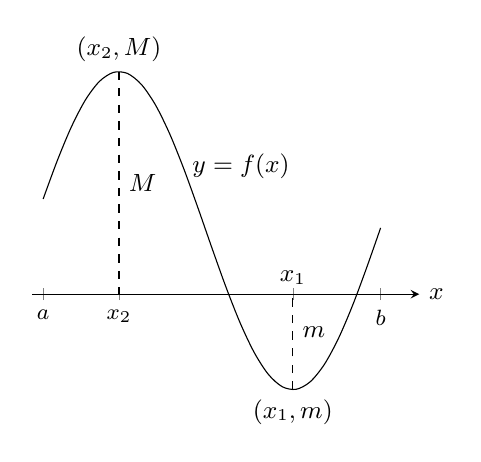
\begin{tikzpicture}[font=\small,declare function={f(\x)=0.4+sin(deg(\x));}]
\pgfmathsetmacro{\kA}{f(1.571)}
\pgfmathsetmacro{\kB}{f(4.713)}
\begin{axis}[clip=false,small,axis lines=middle,xlabel={$x$},xtick={0.2,1.571,4.713,6.3},xticklabels={$a$,$x_2$,,$b$},ytick={\empty},xmin=0,xmax=7,xlabel style={at={(current axis.right of origin)},anchor=west},y axis line style={draw=none}]
\addplot[domain=0.2:6.3,smooth]{f(x)}node[pos=0.4,right]{$y=f(x)$};
\draw(axis cs:1.571,\kA)node[above]{$(x_2,M)$} (axis cs:4.713,\kB)node[below]{$(x_1,m)$};
\draw[dashed](axis cs:1.571,\kA)--(axis cs:1.571,0)node[pos=0.5,right]{$M$};
\draw[dashed](axis cs:4.713,\kB)--(axis cs:4.713,0)node[pos=0.6,right]{$\abs{m}$}node[above]{$x_1$};
\end{axis}
\end{tikzpicture}
\caption{زیادہ سے زیادہ اور کم سے کم قیمتیں اندرونی نقطوں پر ہیں۔}
\end{subfigure}%
\begin{subfigure}{0.5\textwidth}
\centering
\begin{tikzpicture}[font=\small]
\begin{axis}[small,axis lines=middle,xlabel={$x$},xlabel style={at={(current axis.right of origin)},anchor=west},y axis line style={draw=none},xmin=-0.5,xmax=2.5,ymin=0,ymax=1.5,ytick={\empty},xtick={0.2,2},xticklabels={$a$,$b$}]
\draw(axis cs:0.2,1) to [out=-40,in=170] node[pos=0.5,above right]{$y=f(x)$}(axis cs:2,0.5);
\draw[dashed](axis cs:0.2,1)--(axis cs:0.2,0)node[pos=0.5,right]{$M$};
\draw[dashed](axis cs:2,0.5)--(axis cs:2,0)node[pos=0.6,right]{$m$};
\end{axis}
\end{tikzpicture}
\caption{زیادہ سے زیادہ اور کم سے کم آخری نقطوں پر ہے۔}
\end{subfigure}
\begin{subfigure}{0.5\textwidth}
\centering
\begin{tikzpicture}[font=\small,declare function={f(\x)=1+(\x-1)^2;}]
\pgfmathsetmacro{\kA}{f(1)}
\pgfmathsetmacro{\kB}{f(2)}
\begin{axis}[clip=false,small,axis lines=middle,xlabel={$x$},xtick={0.2,1,2},xticklabels={$a$,$x_1$,$b$},ytick={\empty},xmin=0,xmax=2.5,ymin=0,xlabel style={at={(current axis.right of origin)},anchor=west},y axis line style={draw=none}]
\addplot[domain=0.2:2,smooth]{f(x)}node[pos=0.15,above right]{$y=f(x)$};
\draw[dashed](axis cs:1,\kA)--(axis cs:1,0)node[pos=0.5,right]{$m$};
\draw[dashed](axis cs:2,\kB)--(axis cs:2,0)node[pos=0.6,right]{$M$};
\end{axis}
\end{tikzpicture}
\caption{کم سے کم اندرونی نقطہ جبکہ زیادہ سے زیادہ آخری نقطہ ہے۔}
\end{subfigure}%
\begin{subfigure}{0.5\textwidth}
\centering
\begin{tikzpicture}[font=\small,declare function={f(\x)=sin(deg(\x));}]
\pgfmathsetmacro{\kA}{f(0.2)}
\pgfmathsetmacro{\kB}{f(3.142/2)}
\begin{axis}[clip=false,small,axis lines=middle,xlabel={$x$},xtick={0.2,1.571,2.6},xticklabels={$a$,$x_2$,$b$},ytick={\empty},xmin=0,xmax=3,ymin=0,xlabel style={at={(current axis.right of origin)},anchor=west},y axis line style={draw=none}]
\addplot[domain=0.2:2.6,smooth]{f(x)}node[pos=0.15,below right]{$y=f(x)$};
\draw[dashed](axis cs:0.2,\kA)--(axis cs:0.2,0)node[pos=0.5,right]{$m$};
\draw[dashed](axis cs:1.571,\kB)--(axis cs:1.571,0)node[pos=0.6,right]{$M$};
\end{axis}
\end{tikzpicture}
\caption{زیادہ سے زیادہ اندرونی نقطہ جبکہ کم سے کم  آخری نقطہ پر ہے۔}
\end{subfigure}
\caption{زیادہ سے زیادہ اور کم سے کم نقطوں کے چند ممکنہ مقامات۔}
\label{شکل_استعمال_بلند_تر_کم_تر}
\end{figure}

\ابتدا{مثال}\شناخت{مثال_استعمال_انتہائی_سائن_کوسائن}
وقفہ \عددی{[-\pi/2,\pi/2]} پر تفاعل \عددی{f(x)=\cos x} ایک بار زیادہ سے زیادہ قیمت \عددی{1} اور دو بار کم سے کم  قیمت \عددی{0} اختیار کرتا ہے۔اسی وقفے پر  تفاعل \عددی{g(x)=\sin x} ایک بار زیادہ سے زیادہ  قیمت \عددی{1} اور ایک بار کم سے کم قیمت \عددی{-1} اختیار کرتا ہے (شکل \حوالہ{شکل_مثال_استعمال_انتہائی_سائن_کوسائن})۔ 
\begin{figure}
\centering
\begin{tikzpicture}
\begin{axis}[clip=false,small,axis lines=middle,xlabel={$x$},ylabel={$y$},ytick={-1,1},xtick={-1.571,1.571},xticklabels={$-\tfrac{\pi}{2}$,$\tfrac{\pi}{2}$},ymin=-1.2,ymax=1.5,xmin=-2,xmax=2]
\addplot[domain=-1.571:1.571]{cos(deg(x))}node[pos=0.25,above left]{$y=\cos x$};
\addplot[domain=-1.571:1.571]{sin(deg(x))}node[right]{$y=\sin x$};
\addplot[draw=none,mark=*] plot coordinates{(-1.571,0) (1.571,0) (-1.571,-1) (1.571,1) (0,1)};
\end{axis}
\end{tikzpicture}
\caption{ترسیم برائے مثال \حوالہ{مثال_استعمال_انتہائی_سائن_کوسائن}}
\label{شکل_مثال_استعمال_انتہائی_سائن_کوسائن}
\end{figure}
\انتہا{مثال}
%==============================

جیسا شکل \حوالہ{شکل_استعمال_بلند_تر_کم_تر_غیر_یقینی} اور شکل \حوالہ{شکل_استعمال_استمراری_ضروری_ورنہ} واضح کرتے ہیں مسئلہ \حوالہ{مسئلہ_استعمال_بلند_تر_کمتر} میں دائرہ کار کا بند ہونا اور تفاعل کا استمراری ہونا لازمی ہے۔ان کے بغیر مسئلے سے اخذ نتائج غلط ہو سکتے ہیں۔
\begin{figure}
\centering
\begin{minipage}{0.45\textwidth}
\centering
\begin{tikzpicture}[font=\small,declare function={f(\x)=\x;}]
\begin{axis}[clip=false,small,width=6cm,axis lines=middle,xlabel={$x$},ylabel={$y$},xtick={1},ytick={1},xmin=-0.2,xmax=1.25,ymin=-0.2,ymax=1.5,ylabel style={at={(current axis.above origin)},anchor=south}]
\addplot[domain=0:1] {f(x)}node[pos=0.6,below right,align=center]{$y=x$\\  $0<x<1$};
\draw(axis cs:0,0)node[ocirc]{}node[pin=-45:{\RL{کم سے کم قیمت موجود نہیں}}]{} (axis cs:1,1)node[ocirc]{}node[pin=135:{\RL{زیادہ سے زیادہ قیمت موجود نہیں}}]{};
\end{axis}
\end{tikzpicture}
\caption{کھلا وقفہ پر زیادہ سے زیادہ اور کم سے کم قیمتوں کا ہونا یقینی نہیں ہے۔}
\label{شکل_استعمال_بلند_تر_کم_تر_غیر_یقینی}
\end{minipage}\hfill
\begin{minipage}{0.45\textwidth}
\centering
\begin{tikzpicture}[font=\small]
\begin{axis}[clip=false,small,width=6cm,axis lines=middle,xmin=-1.25,xmax=1.5,ymin=-1.25,ymax=1.5]
\addplot[domain=-1:0]{x+1}node[pos=0.4,above left,align=center]{$y=x+1$\\  $-1\le x<0$};
\addplot[domain=0:1]{x-1}node[pos=0.6,below right,align=center]{$y=x-1$\\  $0<x\le 1$};
\draw(axis cs:-1,0)node[circ]{} (axis cs:0,1)node[ocirc]{}node[pin=0:{\RL{زیادہ سے زیادہ  قیمت موجود نہیں}}]{}  (axis cs:0,-1)node[ocirc]{}node[pin=-30:{\RL{کم سے کم قیمت موجود نہیں}}]{}  (axis cs:1,0)node[circ]{};
\end{axis}
\end{tikzpicture}
\caption{واحد ایک نقطہ عدم استمرار کی بنا زیادہ سے زیادہ اور کم سے کم قیمتیں غیر یقینی ہو سکتے ہیں۔}
\label{شکل_استعمال_استمراری_ضروری_ورنہ}
\end{minipage}
\end{figure} 

شکل \حوالہ{شکل_استعمال_استمراری_ضروری_ورنہ} میں تفاعل
\begin{align*}
f(x)=
\begin{cases}
x+1,&-1\le x<0\\ 
0,&x=0\\
x-1,&0<x\le 1
\end{cases}
\end{align*}
دکھایا گیا ہے جو وقفہ \عددی{[-1,1]} پر استمراری ہے ماسوائے واحد نقطہ \عددی{x=0}  پر، جس کی بنا تفاعل کا نا کوئی زیادہ سے زیادہ قیمت اور نا ہی اس کی کوئی کم سے کم قیمت پائی جاتی ہے۔

\جزوحصہء{مقامی بالمقابل مطلق (عالمگیر) انتہا}
شکل \حوالہ{شکل_استعمال_مقامی_مطلق_انتہا} میں تفاعل کے پانچ انتہا نقطے دکھائے گئے ہیں۔اس تفاعل کا کم سے کم نقطہ \عددی{a} پر ہے اگرچہ \عددی{e} پر بھی \عددی{x} کی مقامی قیمتوں کے لحاظ سے \عددی{f} کی قیمت کم ہے۔نقطہ \عددی{c} پر تفاعل کی مقامی زیادہ سے زیادہ قیمت پائی جاتی ہے جبکہ \عددی{d} پر اس کی مطلق زیادہ سے زیادہ قیمت پائی جاتی ہے۔
\begin{figure}
\centering
\begin{tikzpicture}
\draw[-latex](-0.25,0)--(4,0)node[right]{$x$};
\draw(0,0.5) to [out=45,in=180] (1.25,1.3) to [out=0,in=180] (2,1) to [out=0,in=180] (3,2) to [out=-45,in=170] (3.5,1.5);
\draw[dashed] (0,0.5)--(0,0)node[below]{$a$}  (1.25,1.3)--(1.25,0)node[below]{$c$}  (2,1)--(2,0)node[below]{$e$}  (3,2)--(3,0)node[below]{$d$}   (3.5,1.5)--(3.5,0)node[below]{$b$};
\draw(0.75,1.3)--(1.75,1.3)   (1.5,1)--(2.5,1);
\draw(0,0.5)node[left]{\RL{مطلق کم سے کم}};
\draw(1.25,1.3)node[above]{\RL{مقامی زیادہ سے زیادہ}};
\draw(2,1)node[below]{\RL{مقامی کم سے کم}};
\draw(3,2)node[above]{\RL{مطلق زیادہ سے زیادہ}};
\draw(3.5,1.5)node[right]{\RL{مقامی کم سے کم}};
\end{tikzpicture}
\caption{مقامی اور مطلق انتہا۔}
\label{شکل_استعمال_مقامی_مطلق_انتہا}
\end{figure}

\ابتدا{تعریف}\موٹا{مطلق انتہائی قیمتیں}\\
فرض کریں تفاعل \عددی{f} کا دائرہ کار \عددی{D} ہے۔نقطہ \عددی{c} پر تفاعل \عددی{f} کی مطلق زیادہ سے زیادہ قیمت  تب پائی جائے گی جب \عددی{D} میں تمام \عددی{x} کے لئے درج ذیل ہو
\begin{align*}
f(x)\le f(c)
\end{align*}
اور \عددی{D} میں \عددی{c} پر تب \عددی{f} کی مطلق کم سے کم قیمت  پائی جائے گی  جب \عددی{D} میں تمام \عددی{x} کے لئے درج ذیل ہو۔
\begin{align*}
f(x)\ge f(c)
\end{align*} 
\انتہا{تعریف}
%========================

مطلق زیادہ سے زیادہ  اور مطلق کم سے کم کو  مطلق \اصطلاح{انتہا}\فرہنگ{انتہا}\حاشیہب{extrema}\فرہنگ{extrema} کہتے ہیں۔انہیں \اصطلاح{عالمگیر}\فرہنگ{عالمگیر}\حاشیہب{global}\فرہنگ{global} انتہا بھی کہتے ہیں۔

ایک جیسے قاعدہ کے تفاعل کی انتہا قیمتیں مختلف ہو سکتی ہیں۔ انتہا قیمتیں دائرہ کار پر بھی منحصر ہوں گی۔

\ابتدا{مثال}\شناخت{مثال_استعمال_مطلق_قیمت_دائرہ_کار}
\begin{align*}
\begin{array}{cccr}
&\text{قاعدہ تفاعل}&  D\,\text{دائرہ کار}&\multicolumn{1}{c}{\text{مطلق انتہا}}\\
\hline
\text{(ا)}&y=x^2&(-\infty,\infty)& \text{مطلق زیادہ سے زیادہ نہیں ہے جبکہ \عددی{x=0} پر مطلق کم سے کم قیمت \عددی{0} ہے}\\
\text{(ب)}&y=x^2&[0,2]&\text{مطلق زیادہ سے زیادہ قیمت \عددی{x=2} پر \عددی{4} ہے جبکہ \عددی{x=0} پر مطلق کم سے کم قیمت \عددی{0} ہے}\\
\text{(ج)}&y=x^2&(0,2]&\text{مطلق زیادہ سے زیادہ قیمت \عددی{x=2} پر \عددی{4} ہے جبکہ مطلق کم سے کم قیمت موجود نہیں ہے}\\
\text{(د)}&y=x^2&(0,2)&\text{کوئی مطلق قیمت نہیں پایا جاتا ہے}
\end{array}
\end{align*}
شکل \حوالہ{شکل_مثال_استعمال_مطلق_قیمت_دائرہ_کار} دیکھیں۔
\begin{figure}
\centering
\begin{subfigure}{0.5\textwidth}
\centering
\begin{tikzpicture}
\begin{axis}[small,axis lines=middle,xlabel={$x$},ylabel={$y$},xtick={-2,2},ytick={\empty},xlabel style={at={(current axis.right of origin)},anchor=west},xmin=-2.5,xmax=2.5,ymin=-0.2]
\addplot[domain=-2.25:2.25]{x^2};
\draw(axis cs:0,0)node[circ]{};
\draw(axis cs:0,2)node[fill=white,align=center]{$y=x^2$\\  $D:(-\infty,\infty)$};
\end{axis}
\end{tikzpicture}
\caption{مطلق کم سے کم قیمت پائی جاتی ہے}
\end{subfigure}%
\begin{subfigure}{0.5\textwidth}
\centering
\begin{tikzpicture}
\begin{axis}[small,axis lines=middle,xlabel={$x$},ylabel={$y$},xtick={-2,2},ytick={\empty},xlabel style={at={(current axis.right of origin)},anchor=west},xmin=-2.5,xmax=2.5,ymin=-0.2]
\addplot[domain=-2.25:2.25]{x^2};
\draw(axis cs:0,0)node[circ]{}  (axis cs:2,4)node[circ]{};
\draw(axis cs:0,2)node[fill=white,align=center]{$y=x^2$\\  $D:[0,2]$};
\end{axis}
\end{tikzpicture}
\caption{مطلق کم سے کم اور زیادہ سے زیادہ قیمت پائی جاتی ہیں}
\end{subfigure}
\begin{subfigure}{0.5\textwidth}
\centering
\begin{tikzpicture}
\begin{axis}[small,axis lines=middle,xlabel={$x$},ylabel={$y$},xtick={-2,2},ytick={\empty},xlabel style={at={(current axis.right of origin)},anchor=west},xmin=-2.5,xmax=2.5,ymin=-0.2]
\addplot[domain=-2.25:2.25]{x^2};
\draw(axis cs:0,0)node[ocirc]{}  (axis cs:2,4)node[circ]{};
\draw(axis cs:0,2)node[fill=white,align=center]{$y=x^2$\\  $D:(0,2]$};
\end{axis}
\end{tikzpicture}
\caption{مطلق  زیادہ سے زیادہ قیمت پائی جاتی ہے}
\end{subfigure}%
\begin{subfigure}{0.5\textwidth}
\centering
\begin{tikzpicture}
\begin{axis}[small,axis lines=middle,xlabel={$x$},ylabel={$y$},xtick={-2,2},ytick={\empty},xlabel style={at={(current axis.right of origin)},anchor=west},xmin=-2.5,xmax=2.5,ymin=-0.2]
\addplot[domain=-2.25:2.25]{x^2};
\draw(axis cs:0,0)node[ocirc]{}  (axis cs:2,4)node[ocirc]{};
\draw(axis cs:0,2)node[fill=white,align=center]{$y=x^2$\\  $D:(0,2)$};
\end{axis}
\end{tikzpicture}
\caption{نا مطلق زیادہ سے زیادہ اور نا مطلق کم سے کم قیمت پائی جاتی ہے}
\end{subfigure}
\caption{مطلق قیمت اور دائرہ کار (مثال \حوالہ{مثال_استعمال_مطلق_قیمت_دائرہ_کار})۔}
\label{شکل_مثال_استعمال_مطلق_قیمت_دائرہ_کار}
\end{figure}
\انتہا{مثال}
%========================

\ابتدا{تعریف}\موٹا{مقامی انتہا قیمت}\\
تفاعل \عددی{f} کا کھلے دائرہ کار \عددی{D} میں اندرونی نقطہ \عددی{c} پر اس صورت مقامی زیادہ سے زیادہ قیمت پائی جائے گی جب \عددی{D} میں کسی بھی کھلا وقفہ جس میں \عددی{c} پایا جاتا ہو میں تمام \عددی{x} کے لئے
\begin{align*}
f(x)\le f(c)
\end{align*}
ہو جبکہ (انہیں شرائط کے ساتھ) درج ذیل صورت میں  اندرونی نقطہ \عددی{c} پر مقامی زیادہ سے زیادہ قیمت پائی جائے گی۔
\begin{align*}
f(x)\ge f(c)
\end{align*} 
\انتہا{تعریف}
%===========================

ہم مقامی انتہا کی تعریف کو وقفہ کے آخری سروں تک وسعت دے سکتے ہیں۔یوں آخری سر \عددی{c} پر مقامی انتہا سے مراد نصف کھلا وقفہ میں موزوں عدم مساوات کا مطمئن ہونا ہے۔ شکل \حوالہ{شکل_استعمال_مقامی_مطلق_انتہا} میں تفاعل \عددی{f} کا \عددی{c} اور \عددی{d} پر مقامی زیادہ سے زیادہ قیمت جبکہ  \عددی{a}، \عددی{e} اور \عددی{b} پر اس کی مقامی کم سے کم قیمت پائی جاتی ہیں۔

مطلق زیادہ سے زیادہ قیمت بھی مقامی زیادہ سے زیادہ قیمت ہو گی۔مطلق زیادہ سے زیادہ قیمت اپنی پڑوس میں بھی زیادہ سے زیادہ قیمت ہو گی۔یوں تمام مقامی زیادہ سے زیادہ قیمتوں کی جدول میں مطلق زیادہ سے زیادہ قیمت (اگر موجود ہو) بھی پائی جائے گی۔ اسی طرح تمام مقامی کم سے کم قیمتوں کی جدول میں مطلق کم سے کم قیمت (اگر موجود ہو) بھی پائی جائے گی۔

\جزوحصہء{انتہا کا حصول}
جیسا درج ذیل مسئلہ سمجھاتا ہے تفاعل کے  انتہا کی حصول کے لئے صرف چند قیمتوں کی تحقیق ضروری ہو گی۔

\ابتدا{مسئلہ}\شناخت{مسئلہ_استعمال_یک_درجی_تفرق_انتہا}\موٹا{یک درجی مسئلہ برائے مقامی انتہا}
فرض کریں  تفاعل \عددی{f} کے دائرہ کار کی اندرونی نقطہ \عددی{c} پر \عددی{f} کی کم سے کم یا زیادہ سے زیادہ قیمت پائی جاتی ہو اور \عددی{c} پر \عددی{f'} معین ہو تب درج ذیل ہو گا۔
\begin{align*}
f'(c)=0
\end{align*} 
\انتہا{مسئلہ}
%=====================
\ابتدا{ثبوت}
یہ دکھانے کی خاطر کہ مقامی انتہا پر \عددی{f'(c)} کی قیمت صفر ہو گی ہم  دکھاتے ہیں کہ \عددی{f'(c)} مثبت نہیں ہو سکتا ہے اور  کہ \عددی{f'(c)} منفی نہیں ہو سکتا ہے۔صفر وہ  واحد عدد ہے جو نا مثبت اور نا منفی ہے لہٰذا \عددی{f'(c)} صفر ہو گا۔   

فرض کریں کہ \عددی{c} پر \عددی{f} کی مقامی زیادہ سے زیادہ قیمت پائی جاتی ہے (شکل \حوالہ{شکل_مسئلہ_استعمال_یک_درجی_تفرق_انتہا})۔ یوں \عددی{c} کے قریبی پڑوس میں تمام \عددی{x} پر \عددی{f(x)-f(c)\le 0} ہو گا۔چونکہ \عددی{c} اندرونی نقطہ ہے لہٰذا \عددی{f'(c)} کی تعریف درج ذیل دو طرفہ حد ہو گی۔
\begin{align*}
\lim_{x\to c}\frac{f(x)-f(c)}{x-c}
\end{align*}
اس کا مطلب ہے کہ \عددی{x=c} پر دائیں ہاتھ حد اور بائیں ہاتھ حد دونوں موجود اور \عددی{f'(c)} کے برابر ہیں۔ان حد پر علیحدہ علیحدہ غور کرتے ہیں۔چونکہ \عددی{c} کے دائیں جانب \عددی{x-c>0} اور \عددی{f(x)\le f(c)} ہیں لہٰذا
\begin{align}\label{مساوات_استعمال_یک_درجی_تفرق_الف}
f'(c)=\lim_{x\to c^+}\frac{f(x)-f(c)}{x-c}\le 0
\end{align}
ہو گا۔اسی طرح \عددی{c} کے بائیں جانب \عددی{x-c<0} اور \عددی{f(x)\le f(c)} ہیں لہٰذا
\begin{align}\label{مساوات_استعمال_یک_درجی_تفرق_ب}
f'(c)=\lim_{x\to c^-}\frac{f(x)-f(c)}{x-c}\ge 0
\end{align}
ہو گا۔مساوات \حوالہ{مساوات_استعمال_یک_درجی_تفرق_الف} اور مساوات \حوالہ{مساوات_استعمال_یک_درجی_تفرق_ب} کو ملا کر \عددی{f'(c)=0} ملتا ہے۔

یوں مقامی زیادہ سے زیادہ قیمت کے لئے مسئلہ ثابت ہوا۔مقامی کم سے کم قیمت کے لئے مسئلہ ثابت کرنے کے لئے \عددی{f(x)\ge f(c)} استعمال کرنا ہو گا جس سے مساوات \حوالہ{مساوات_استعمال_یک_درجی_تفرق_الف} اور مساوات \حوالہ{مساوات_استعمال_یک_درجی_تفرق_ب} کی عدم مساوات الٹ ہو جاتی ہیں۔
\begin{figure}
\centering
\begin{tikzpicture}[font=\small,y=2cm,x=2cm,declare function={f(\x)=1.5-\x*\x;}]
\pgfmathsetmacro{\kA}{f(0.2)}
\pgfmathsetmacro{\kB}{f(0.4)}
\pgfmathsetmacro{\kC}{f(0.6)}
\draw[-latex] (-1.5,0)--(1.5,0)node[right]{$x$};
\draw[name path=kC,domain=-1:1] plot ({\x},{1.5-\x*\x})node[right]{$y=f(x)$};
\draw(-1,1.5)--(1,1.5);
\draw[shorten <=-0.5cm, shorten >=-0.5cm](0,1.5)--(0.2,\kA);
\draw[shorten <=-0.5cm, shorten >=-0.5cm](0,1.5)--(0.4,\kB);
\draw[shorten <=-0.5cm, shorten >=-0.5cm](0,1.5)--(0.6,\kC);
\draw[shorten <=-0.5cm, shorten >=-0.5cm](0,1.5)--(-0.2,\kA);
\draw[shorten <=-0.5cm, shorten >=-0.5cm](0,1.5)--(-0.4,\kB);
\draw[shorten <=-0.5cm, shorten >=-0.5cm](0,1.5)--(-0.6,\kC);
\draw[dashed] (-0.6,\kC)--(-0.6,0)node[below]{$x$};
\draw[dashed] (0,1.5)--(0,0)node[below]{$c$};
\draw[dashed] (0.6,\kC)--(0.6,0)node[below]{$x$};
\draw(0,1.5)node[pin=90:{\RL{مقامی انتہا}}]{};
\draw(-0.5,0.5)node[fill=white,align=center]{\RL{غیر منفی}\\ \RL{ڈھلوان سیکنٹ}};
\draw(0.5,0.5)node[fill=white,align=center]{\RL{غیر مثبت}\\ \RL{ڈھلوان سیکنٹ}};
\end{tikzpicture}
\caption{اندرونی نقطہ پر مقامی انتہا پر ڈھلوان صفر ہو گی (مسئلہ \حوالہ{مسئلہ_استعمال_یک_درجی_تفرق_انتہا})۔}
\label{شکل_مسئلہ_استعمال_یک_درجی_تفرق_انتہا}
\end{figure}
\انتہا{ثبوت}
%======================

مسئلہ \حوالہ{مسئلہ_استعمال_یک_درجی_تفرق_انتہا} کہتا ہے کہ اندرونی انتہا پر اگر تفرق معین ہو تب \عددی{f'(c)=0} ہو گا۔ یوں تفاعل کی انتہا (مقامی یا عالمگیر) صرف درج ذیل نقطوں پر ہو سکتی ہیں۔
\begin{enumerate}[1.]
\item
اندرونی نقطہ جہاں \عددی{f'=0} ہو۔\\
\item
اندرونی نقطہ جہاں \عددی{f'} غیر معین ہو۔\\
\item
\عددی{f} کے دائرہ کار کے آخری سروں پر۔
\end{enumerate}

درج ذیل تعریف ان نتائج کو مختصراً پیش کرنے میں مدد کرتی ہے۔

\ابتدا{تعریف}
تفاعل \عددی{f} کے دائرہ کار میں ایسا اندرونی نقطہ جہاں \عددی{f'} غیر معین یا صفر ہو کو \اصطلاح{نقطہ فاصل}\فرہنگ{نقطہ فاصل}\حاشیہب{critical point}\فرہنگ{critical point} کہتے ہیں۔ 
\انتہا{تعریف}

\موٹا{خلاصہ}\\
تفاعل کی انتہا قیمتیں صرف تفاعل کی دائرہ کار میں نقطہ فاصل اور آخری نقطوں  پر پائی جا سکتی ہیں۔ 

عموماً بند دائرہ کار پر تفاعل  کی انتہا  مطلوب ہو گی۔ مسئلہ \حوالہ{مسئلہ_استعمال_بلند_تر_کمتر} ہمیں یقین دلاتا ہے کہ ایسی قیمتیں موجود ہوں گی؛  مسئلہ \حوالہ{مسئلہ_استعمال_یک_درجی_تفرق_انتہا} کہتا ہے کہ یہ صرف آخری نقطوں پر اور نقطہ فاصل پر پائی جائیں گی۔اس قسم کے نقطے عموماً چند ہوں گے جن کی فہرست تیار کر کے دیکھا جا سکتا ہے کہ آیا نقطہ پر زیادہ سے زیادہ یا کم سے کم قیمت پائی جاتی ہے۔

\ابتدا{مثال}
دائرہ کار \عددی{[-2,1]} پر تفاعل \عددی{f(x)=x^2} کی مطلق زیادہ سے زیادہ اور مطلق کم سے کم قیمتیں تلاش کریں۔\\
حل:\quad
تفاعل پورے دائرہ کار پر قابل تفرق ہے لہٰذا واحد نقطہ فاصل \عددی{f'(x)=2x=0} یعنی \عددی{x=0} پر ہو گا۔ہمیں تفاعل کی قیمتیں نقطہ فاصل \عددی{x=0} اور آخری نقطوں \عددی{x=-2} اور \عددی{x=1} پر دیکھنی ہوں گی۔
\begin{align*}
f(0)&=0&&\text{نقطہ فاصل پر قیمت}\\
f(-2)&=4&&\text{آخری نقطہ پر قیمت}\\
f(1)&=1&&\text{آخری نقطہ پر قیمت}
\end{align*}
تفاعل کی مطلق زیادہ سے زیادہ قیمت \عددی{4} ہے جو نقطہ \عددی{x=-2} پر پائی جاتی ہے جبکہ اس کی مطلق کم سے کم قیمت \عددی{0} ہے جو نقطہ \عددی{x=0} پر پائی جاتی ہے۔
\انتہا{مثال}
%===================
\ابتدا{مثال}\شناخت{مثال_استعمال_مطلق_انتہا_الف}
دائرہ کار \عددی{[-2,1]} پر تفاعل \عددی{g(t)=8t-t^4} کی مطلق زیادہ سے زیادہ اور مطلق کم سے کم قیمت تلاش کریں۔\\
حل:\quad تفرق پورے دائرہ کار پر قابل تفرق ہے لہٰذا نقطہ فاصل صرف وہاں ہو گا جہاں \عددی{g'(t)=0} ہو۔ اس مساوات کو حل کرتے ہوئے
\begin{align*}
g'(t)&=8-4t^3=0\\
t^3&=2\\
t&=2^{1/3}
\end{align*}
ملتا ہے جو دائرہ کار کے اندر نہیں ہے۔یوں تفاعل کے مقامی انتہا قیمتیں آخری نقطوں پر پائی جائیں گی: (شکل \حوالہ{شکل_مثال_استعمال_مطلق_انتہا_الف})
\begin{align*}
g(-2)&=-32&&\text{مطلق کم سے کم قیمت}\\
g(1)&=7&&\text{مطلق زیادہ سے زیادہ قیمت}
\end{align*}
%
\begin{figure}
\centering
\begin{minipage}{0.45\textwidth}
\centering
\begin{tikzpicture}[font=\small]
\begin{axis}[clip=false,small,axis lines=middle,xlabel={$t$},ylabel={$y$},xtick={-2,1},ytick={-32,7},xmin=-2.5,xmax=1.5,ymin=-35,ymax=9]
\addplot[domain=-2:1]{8*x-x^4}node[pos=0.25,right]{$g(t)=8t-t^4$};
\draw(axis cs:1,7)node[circ]{}node[above]{$(1,7)$}  (axis cs:-2,-32)node[circ]{}node[below]{$(-2,-32)$};
\end{axis}
\end{tikzpicture}
\caption{ترسیم برائے مثال \حوالہ{مثال_استعمال_مطلق_انتہا_الف}}
\label{شکل_مثال_استعمال_مطلق_انتہا_الف}
\end{minipage}\hfill
\begin{minipage}{0.45\textwidth}
\centering
\begin{tikzpicture}[font=\small]
\begin{axis}[clip=false,small,axis lines=middle,xlabel={$x$},ylabel={$y$},xtick={-2,-1,1,2,3},ytick={1,2},xmin=-3,xmax=4.5]
\addplot[domain=-0.5:0]{(x^2)^(1/3)};
\addplot[domain=0:0.5]{(x^2)^(1/3)};
\addplot[domain=-2:-0.5]{(x^2)^(1/3)};
\addplot[domain=0.5:3]{(x^2)^(1/3)}node[pos=0.25,right]{$y=x^{2/3}$};
\draw(axis cs:-2,1.587)node[circ]{}node[above]{\RL{مقامی زیادہ سے زیادہ}}  (axis cs:3,2.08)node[circ]{}node[above]{\RL{مطلق اور مقامی زیادہ سے زیادہ}};
\end{axis}
\end{tikzpicture}
\caption{ترسیم برائے مثال \حوالہ{مثال_استعمال_مطلق_انتہا_ب}}
\label{شکل_مثال_استعمال_مطلق_انتہا_ب}
\end{minipage}
\end{figure}
\انتہا{مثال}
%======================
\ابتدا{مثال}\شناخت{مثال_استعمال_مطلق_انتہا_ب}
تفاعل \عددی{h(x)=x^{2/3}} کی  \عددی{[-2,-3]} پر مطلق انتہا تلاش کریں۔\\
حل:\quad
یک درجی تفرق
\begin{align*}
h'(x)=\frac{2}{3}x^{-1/3}=\frac{2}{3x^{1/3}}
\end{align*}
کا صفر نہیں پایا جاتا ہے البتہ \عددی{x=0} پر یہ غیر معین ہے۔اس نقطہ پر اور آخری نقطوں \عددی{x=-2} اور \عددی{x=3} پر تفاعل کی قیمتیں درج ذیل ہیں۔
\begin{align*}
h(0)&=0\\
h(-2)&=(-2)^{2/3}=4^{1/3}\\
h(3)&=(3)^{2/3}=9^{1/3}
\end{align*}
مطلق زیادہ سے زیادہ قیمت \عددی{9^{1/3}} ہے جو نقطہ \عددی{x=3} پر پائی جاتی ہے جبکہ مطلق کم سے کم قیمت \عددی{0} ہے جو نقطہ \عددی{x=0} پر پائی جاتی ہے  (شکل \حوالہ{شکل_مثال_استعمال_مطلق_انتہا_ب})۔
\انتہا{مثال}
%=====================

اگرچہ تفاعل کی انتہا صرف نقطہ فاصل اور آخری نقطوں پر پائی جا سکتی ہیں، ضروری نہیں ہے کہ ہر نقطہ فاصل یا ہر آخری نقطہ  پر انتہا قیمت پائی جاتی ہو۔ شکل \حوالہ{شکل_مثال_استعمال_نقطہ_فاصل_نہیں_الف} اور شکل \حوالہ{شکل_مثال_استعمال_نقطہ_فاصل_نہیں_ب} اندرونی نقطوں کے لئے اس حقیقت کی وضاحت کرتی ہے۔
\begin{figure}
\centering
\begin{minipage}{0.45\textwidth}
\centering
\begin{tikzpicture}
\begin{axis}[small,axis lines=middle,xlabel={$x$},ylabel={$y$},xtick={-1,1},ytick={-1,1}]
\addplot[domain=0:0.01]{x^(1/3)};
\addplot[domain=0:0.01]({-x},{-x^(1/3)});
\addplot[domain=0.01:0.5]{x^(1/3)};
\addplot[domain=0.01:0.5]({-x},{-x^(1/3)});
\addplot[domain=0.5:2]{x^(1/3)}node[pos=0.5,below]{$y=x^{1/3}$};
\addplot[domain=0.5:2]({-x},{-x^(1/3)});
\end{axis}
\end{tikzpicture}
\caption{نقطہ فاصل \عددی{x=0} پر انتہائی قیمت نہیں پائی جاتی ہے۔}
\label{شکل_مثال_استعمال_نقطہ_فاصل_نہیں_الف}
\end{minipage}\hfill
\begin{minipage}{0.45\textwidth}
\centering
\begin{tikzpicture}
\begin{axis}[small,axis lines=middle,xlabel={$x$},ylabel={$y$},xtick={-1,1},ytick={-1,1},xmin=-1.5,xmax=1.5,ymin=-1.5,ymax=1.5]
\addplot[domain=-1:1]{x^3}node[pos=0.9,left]{$y=x^3$};
\end{axis}
\end{tikzpicture}
\caption{
\عددی{x=0} پر \عددی{y=x^3} کا کوئی انتہا نہیں پایا جاتا ہے اگرچہ اس نقطے پر \عددی{y'=3x^2=0} ہے۔
}
\label{شکل_مثال_استعمال_نقطہ_فاصل_نہیں_ب}
\end{minipage}
\end{figure} 

\حصہء{سوالات}
\موٹا{ترسیم سے انتہائی نقطوں کا حصول}\\
کیا سوال \حوالہ{سوال_استعمال_ترسیم_سے_مطلق_الف} تا سوال \حوالہ{سوال_استعمال_ترسیم_سے_مطلق_ب} میں \عددی{[a,b]} کے بیچ تفاعل کے مطلق انتہائی قیمتیں پائی جاتی ہیں؟ سمجھائیں کہ آپ کے جواب اور مسئلہ \حوالہ{مسئلہ_استعمال_بلند_تر_کمتر} میں کس طرح تضاد نہیں پایا جاتا ہے۔

\begin{figure}
\centering
\begin{subfigure}{0.33\textwidth}
\centering
\begin{tikzpicture}[x=0.6cm][x=0.6cm]
\draw[-latex] (-0.25,0)--(4.25,0)node[right]{$x$};
\draw[-latex](0,-0.2)--(0,2)node[above]{$y$};
\draw(1,0.5)node[circ]{} to [out=30,in=180] (2,1)node[above]{$y=h(x)$} to [out=0,in=180] (3,0.25) to [out=0,in=-120](4,2)node[circ]{};
\foreach \x/\l in {1/a,2/{c_1},3/{c_2},4/b}{\draw(\x,0)node[below]{$\l$}--++(0,0.1);}
\end{tikzpicture}
\caption{}
\end{subfigure}%
\begin{subfigure}{0.33\textwidth}
\centering
\begin{tikzpicture}[x=0.6cm]
\draw[-latex] (-0.25,0)--(4.25,0)node[right]{$x$};
\draw[-latex](0,-0.2)--(0,2)node[above]{$y$};
\draw(1,1)node[circ]{} to [out=30,in=180] (2.5,2) to [out=0,in=150] node[pos=0.5,right]{$y=f(x)$}(4,0.5)node[circ]{};
\foreach \x/\l in {1/a,2.5/{c},4/b}{\draw(\x,0)node[below]{$\l$}--++(0,0.1);}
\end{tikzpicture}
\caption{}
\end{subfigure}%
\begin{subfigure}{0.33\textwidth}
\centering
\begin{tikzpicture}[x=0.6cm]
\draw[-latex] (-0.25,0)--(4.25,0)node[right]{$x$};
\draw[-latex](0,-0.2)--(0,2)node[above]{$y$};
\draw(1,0.5)node[ocirc]{} to [out=20,in=-110] (3,2) to [out=-70,in=150] node[pos=0.2,right]{$y=f(x)$}(4,0.5)node[ocirc]{};
\foreach \x/\l in {1/a,3/{c},4/b}{\draw(\x,0)node[below]{$\l$}--++(0,0.1);}
\end{tikzpicture}
\caption{}
\end{subfigure}
\begin{subfigure}{0.33\textwidth}
\centering
\begin{tikzpicture}[x=0.6cm]
\draw[-latex] (-0.25,0)--(4.25,0)node[right]{$x$};
\draw[-latex](0,-0.2)--(0,2)node[above]{$y$};
\draw(1,2)node[ocirc]{} to [out=-50,in=180] (3,0.5)node[ocirc]{} to [out=0,in=-140] node[pos=1,above]{$y=h(x)$}(4,1)node[ocirc]{};
\draw(3,1)node[circ]{};
\foreach \x/\l in {1/a,3/{c},4/b}{\draw(\x,0)node[below]{$\l$}--++(0,0.1);}
\end{tikzpicture}
\caption{}
\end{subfigure}%
\begin{subfigure}{0.33\textwidth}
\centering
\begin{tikzpicture}[x=0.6cm]
\draw[-latex] (-0.25,0)--(4.25,0)node[right]{$x$};
\draw[-latex](0,-0.2)--(0,2)node[above]{$y$};
\draw(1,0.5)node[circ]{} to [out=80,in=-150] (2,2)node[circ]{}  (2,1.5)node[ocirc]{}to [out=-30,in=170] node[pos=0.5,above right]{$y=g(x)$}(4,1)node[circ]{};
\foreach \x/\l in {1/a,2/{c},4/b}{\draw(\x,0)node[below]{$\l$}--++(0,0.1);}
\end{tikzpicture}
\caption{}
\end{subfigure}%
\begin{subfigure}{0.33\textwidth}
\centering
\begin{tikzpicture}[x=0.6cm]
\draw[-latex] (-0.25,0)--(4.25,0)node[right]{$x$};
\draw[-latex](0,-0.2)--(0,2)node[above]{$y$};
\draw(1,1.5)node[ocirc]{} to [out=-20,in=110] (2.5,0.5) to [out=80,in=-150] node[pos=1,above left]{$y=g(x)$}(4,1.5)node[circ]{};
\draw(1,2)node[circ]{};
\foreach \x/\l in {1/a,2.5/{c},4/b}{\draw(\x,0)node[below]{$\l$}--++(0,0.1);}
\end{tikzpicture}
\caption{}
\end{subfigure}
\caption{اشکال برائے سوال \حوالہ{سوال_استعمال_ترسیم_سے_مطلق_الف} تا سوال \حوالہ{سوال_استعمال_ترسیم_سے_مطلق_ب}}
\label{شکل_سوال_استعمال_ترسیم_سے_مطلق_الف}
\end{figure}
%
\ابتدا{سوال}\شناخت{سوال_استعمال_ترسیم_سے_مطلق_الف}
شکل \حوالہ{شکل_سوال_استعمال_ترسیم_سے_مطلق_الف}-ا\\
جواب:\quad
\عددی{x=c_2} پر مطلق کم سے کم؛ \عددی{x=b} پر  مطلق زیادہ سے زیادہ۔
\انتہا{سوال}
%===================
\ابتدا{سوال}
شکل \حوالہ{شکل_سوال_استعمال_ترسیم_سے_مطلق_الف}-ب
\انتہا{سوال}
%======================================
\ابتدا{سوال}
شکل \حوالہ{شکل_سوال_استعمال_ترسیم_سے_مطلق_الف}-ج\\
جواب:\quad
\عددی{x=c} پر مطلق زیادہ سے زیادہ؛ مطلق کم سے کم غیر موجود۔
\انتہا{سوال}
%=======================================
\ابتدا{سوال}
شکل \حوالہ{شکل_سوال_استعمال_ترسیم_سے_مطلق_الف}-د
\انتہا{سوال}
%=======================================
\ابتدا{سوال}
شکل \حوالہ{شکل_سوال_استعمال_ترسیم_سے_مطلق_الف}-ہ\\
جواب:\quad
\عددی{x=a} پر مطلق کم سے کم؛ \عددی{x=c} پر  مطلق زیادہ سے زیادہ۔
\انتہا{سوال}
%=======================================
\ابتدا{سوال}\شناخت{سوال_استعمال_ترسیم_سے_مطلق_ب}
شکل \حوالہ{شکل_سوال_استعمال_ترسیم_سے_مطلق_الف}-و
\انتہا{سوال}
%=======================

\موٹا{بند وقفہ پر مطلق انتہا}
%=======================================

سوال \حوالہ{سوال_استعمال_مطلق_قیمتیں_تلاش_الف} تا سوال \حوالہ{سوال_استعمال_مطلق_قیمتیں_تلاش_ب} میں دیے گئے وقفے پر تفاعل کی مطلق انتہائی قیمتیں تلاش کریں۔تفاعل کو ترسیم کرتے ہوئے انتہائی نقطوں کی نشاندہی کریں۔

\ابتدا{سوال}\شناخت{سوال_استعمال_مطلق_قیمتیں_تلاش_الف}
$f(x)=\frac{2}{3}x-5,\quad -2\le x\le 3$\\
جواب:\quad
\عددی{x=-3} پر مطلق زیادہ سے زیادہ؛ \عددی{x=-\tfrac{19}{3}} پر  مطلق کم سے کم۔شکل \حوالہ{شکل_سوال_استعمال_مطلق_قیمتیں_تلاش_الف}-ا
\انتہا{سوال}
%======================
\ابتدا{سوال}
$f(x)=-x-4,\quad -4\le x\le 1$
\انتہا{سوال}
%======================
\ابتدا{سوال}
$f(x)=x^2-1,\quad -1\le x\le 2$\\
جواب:\quad
مطلق زیادہ سے زیادہ:\عددی{3}، مطلق کم سے کم :\عددی{-1}، شکل \حوالہ{شکل_سوال_استعمال_مطلق_قیمتیں_تلاش_الف}-ب
\انتہا{سوال}
%======================
\ابتدا{سوال}
$f(x)=4-x^2,\quad -3\le x\le 1$
\انتہا{سوال}
%======================
\ابتدا{سوال}
$F(x)=-\tfrac{1}{x^2},\quad 0.5\le x\le 2$\\
جواب:\quad
مطلق زیادہ سے زیادہ:\عددی{-0.25}، مطلق کم سے کم :\عددی{-4}، شکل \حوالہ{شکل_سوال_استعمال_مطلق_قیمتیں_تلاش_الف}-ج
\انتہا{سوال}
%======================
\ابتدا{سوال}
$F(x)=-\tfrac{1}{x},\quad -2\le x\le -1$
\انتہا{سوال}
%======================
\ابتدا{سوال}
$h(x)=\sqrt[3]{x},\quad -1\le x\le 8$\\
جواب:\quad
مطلق زیادہ سے زیادہ:\عددی{2}، مطلق کم سے کم :\عددی{-1}، شکل \حوالہ{شکل_سوال_استعمال_مطلق_قیمتیں_تلاش_الف}-د
\انتہا{سوال}
%======================
\ابتدا{سوال}
$h(x)=-3x^{2/3},\quad -1\le x\le 1$
\انتہا{سوال}
%======================
\ابتدا{سوال}
$g(x)=\sqrt{4-x^2},\quad -2\le x\le 1$\\
جواب:\quad
مطلق زیادہ سے زیادہ:\عددی{2}، مطلق کم سے کم :\عددی{0}، شکل \حوالہ{شکل_سوال_استعمال_مطلق_قیمتیں_تلاش_الف}-ہ
\انتہا{سوال}
%======================
\ابتدا{سوال}
$g(x)=-\sqrt{5-x^2},\quad -\sqrt{5}\le x\le 0$
\انتہا{سوال}
%======================
\ابتدا{سوال}
$f(\theta)=\sin\theta,\quad -\tfrac{\pi}{2}\le \theta \le \tfrac{5\pi}{6}$\\
جواب:\quad
مطلق زیادہ سے زیادہ:\عددی{1}، مطلق کم سے کم :\عددی{-1}، شکل \حوالہ{شکل_سوال_استعمال_مطلق_قیمتیں_تلاش_الف}-و
\انتہا{سوال}
%======================
\ابتدا{سوال}
$f(x)=\tan\theta,\quad -\tfrac{\pi}{3}\le \theta\le \tfrac{\pi}{4}$
\انتہا{سوال}
%======================
\ابتدا{سوال}
$g(x)=\csc x,\quad -\tfrac{\pi}{3}\le x \le \tfrac{2\pi}{3}$\\
جواب:\quad
مطلق زیادہ سے زیادہ:\عددی{\tfrac{2}{\sqrt{3}}}، مطلق کم سے کم :\عددی{-1}، شکل \حوالہ{شکل_سوال_استعمال_مطلق_قیمتیں_تلاش_الف}-ز
\انتہا{سوال}
%======================
\ابتدا{سوال}
$g(x)=\sec x,\quad -\tfrac{\pi}{3}\le x\le \tfrac{\pi}{6}$
\انتہا{سوال}
%======================
\ابتدا{سوال}
$f(t)=2-\abs{t},\quad -1\le t\le 3$\\
جواب:\quad
مطلق زیادہ سے زیادہ:\عددی{2}، مطلق کم سے کم :\عددی{-1}، شکل \حوالہ{شکل_سوال_استعمال_مطلق_قیمتیں_تلاش_الف}-ح
\انتہا{سوال}
%======================
\ابتدا{سوال}\شناخت{سوال_استعمال_مطلق_قیمتیں_تلاش_ب}
$f(t)=\abs{t-5},\quad -4\le t\le 7$
\انتہا{سوال}
%======================
\begin{figure}
\centering
\begin{subfigure}{0.22\textwidth}
\centering
\begin{tikzpicture}[font=\small]
\begin{axis}[clip=false,small,width=4cm,axis lines=middle,xmin=-3.5,xmax=4.5,ymax=0.5,ymin=-7.5,xlabel={$x$},ylabel={$y$},xlabel style={at={(current axis.right of origin)},anchor=west},ylabel style={at={(current axis.above origin)},anchor=south},ytick={-7,-3},xtick={-2,3}]
\addplot[] plot coordinates {(-2,-19/3) (3,-3)};
\draw(axis cs:3,-7)node[align=center,font=\tiny]{$y=\tfrac{2}{3}x-5$\\  $-2\le x\le 3$};
\draw(axis cs:-2,-19/3)node[circ]{}node[above,align=center,font=\tiny]{\RL{مطلق کم سے کم}\\  $(-2,-\tfrac{19}{3})$};
\draw(axis cs:3,-3)node[circ]{}node[below,align=center,font=\tiny]{$(3,-3)$\\   \RL{مطلق زیادہ سے زیادہ}};
\end{axis}
\end{tikzpicture}
\caption{}
\end{subfigure}\hfill
\begin{subfigure}{0.22\textwidth}
\centering
\begin{tikzpicture}[font=\small]
\begin{axis}[clip=false,small,width=4cm,axis lines=middle,xlabel={$x$},ylabel={$y$},xlabel style={at={(current axis.right of origin)},anchor=west},ylabel style={at={(current axis.above origin)},anchor=south},ymin=-1.5,ymax=3.5,xmin=-1.5,xmax=2.5]
\addplot[domain=-1:2]{x^2-1}node[circ]{}node[left,align=center,font=\tiny]{\RL{مطلق زیادہ سے زیادہ}\\  $(2,3)$} node[pos=0.75,right,align=center,font=\tiny]{$y=x^2-1$\\   $-1\le x\le 2$};
\draw(axis cs:-1,0)node[circ]{};
\draw(axis cs:0,-1)node[circ]{}node[below right,align=center,font=\tiny]{$(0,-1)$\\   \RL{مطلق کم سے کم}};
\end{axis}
\end{tikzpicture}
\caption{}
\end{subfigure}\hfill
\begin{subfigure}{0.22\textwidth}
\centering
\begin{tikzpicture}[font=\small]
\begin{axis}[clip=false,small,width=4cm,axis lines=middle,xlabel={$x$},ylabel={$y$},xlabel style={at={(current axis.right of origin)},anchor=west},ylabel style={at={(current axis.above origin)},anchor=south},xmin=0,ymax=0.5,xmax=2.9]
\addplot[domain=0.5:2]{-1/(x^2)}node[circ]{}node[below right,align=center,font=\tiny]{\RL{مطلق زیادہ سے زیادہ}\\  $(2,-0.25)$} 
node[pos=0.5,right,align=center,font=\tiny]{$y=-\frac{1}{x^2}$\\  $0.5\le x\le 2$};
\draw(axis cs:0.5,-4)node[circ]{}node[right,align=center,font=\tiny]{$(0.5,-4)$\\   \RL{مطلق کم سے کم}};
\end{axis}
\end{tikzpicture}
\caption{}
\end{subfigure}\hfill
\begin{subfigure}{0.22\textwidth}
\centering
\begin{tikzpicture}[font=\small]
\begin{axis}[clip=false,small,width=4cm,axis lines=middle,xlabel={$x$},ylabel={$y$},xlabel style={at={(current axis.right of origin)},anchor=west},ylabel style={at={(current axis.above origin)},anchor=south},xmin=-1.75,xmax=9,ymin=-1.5,ymax=2.5,xtick={-1,8},xticklabels={,$8$},ytick={-1,2},yticklabels={,$2$}]
\addplot[domain=0:0.5]{x^(1/3)};
\addplot[domain=0:0.5]({-x},{-x^(1/3)});
\addplot[domain=0.5:8]{x^(1/3)}node[circ]{}node[right,align=center,font=\tiny]{$(8,2)$\\  \RL{مطلق زیادہ سے زیادہ}};
\addplot[domain=0.5:1]({-x},{-x^(1/3)})node[circ]{}node[below,align=center,font=\tiny]{$(-1,-1)$\\   \RL{مطلق کم سے کم}};
\draw(axis cs:2,1)node[right,align=center,font=\tiny]{$y=\sqrt[3]{x}$\\  $-1\le x\le 8$};
\end{axis}
\end{tikzpicture}
\caption{}
\end{subfigure}
\begin{subfigure}{0.22\textwidth}
\centering
\begin{tikzpicture}[font=\small]
\begin{axis}[clip=false,small,width=4cm,axis lines=middle,xlabel={$x$},ylabel={$y$},xlabel style={at={(current axis.right of origin)},anchor=west},ylabel style={at={(current axis.above origin)},anchor=south},xmin=-2.5,xmax=1.5,ymax=2.5]
\addplot[domain=-2:-1.5]{sqrt(4-x^2)};
\addplot[domain=-1.5:1]{sqrt(4-x^2)}node[pos=0.5,above left,align=center,font=\tiny]{$y=\sqrt{4-x^2}$\\ $-2\le x\le 1$};
\draw(axis cs:-2,0)node[circ]{}node[above right,align=center,font=\tiny]{$(-2,0)$\\   \RL{مقامی کم سے کم}};
\draw(axis cs:0,2)node[circ]{}node[above right,align=center,font=\tiny]{\RL{مقامی زیادہ سے زیادہ}\\   $(0,2)$};
\draw(axis cs:1,1.732)node[circ]{};
\end{axis}
\end{tikzpicture}
\caption{}
\end{subfigure}\hfill
\begin{subfigure}{0.22\textwidth}
\centering
\begin{tikzpicture}[font=\small]
\begin{axis}[clip=false,small,width=4cm,axis lines=middle,xlabel={$\theta$},ylabel={$y$},xlabel style={at={(current axis.right of origin)},anchor=west},ylabel style={at={(current axis.above origin)},anchor=south},xtick={-1.57,1.57,2.618},xticklabels={$-\tfrac{\pi}{2}$,$\tfrac{\pi}{2}$,$\tfrac{5\pi}{6}$},xmin=-2,xmax=3,ymin=-1.5,ymax=1.5]
\addplot[domain=-1.57:2.618]{sin(deg(x))}node[circ]{};
\draw(axis cs:-1.57,-1)node[circ]{}node[below,align=center,font=\tiny]{$(-\tfrac{\pi}{2},-1)$\\  \RL{مقامی کم سے کم}};
\draw(axis cs:1.57,1)node[circ]{}node[above right,align=center,font=\tiny]{\RL{مقامی زیادہ سے زیادہ}\\   $(\tfrac{\pi}{2},1)$};
\draw(axis cs:1.57,-1.5)node[align=center,font=\tiny]{$y=\sin \theta$\\  $ -\tfrac{\pi}{2}\le \theta \le \tfrac{5\pi}{6}$};
\end{axis}
\end{tikzpicture}
\caption{}
\end{subfigure}\hfill
\begin{subfigure}{0.22\textwidth}
\centering
\begin{tikzpicture}[font=\small]
\begin{axis}[clip=false,small,width=4cm,axis lines=middle,xlabel={$x$},ylabel={$y$},xlabel style={at={(current axis.right of origin)},anchor=west},ylabel style={at={(current axis.above origin)},anchor=south},xmin=0,ymin=0,xmax=2.2,xtick={1.04,1.57,2.09},xticklabels={$\tfrac{\pi}{3}$,$\tfrac{\pi}{2}$,$\tfrac{2\pi}{3}$}]
\addplot[domain=1.04:2.09]{cosec(deg(x))}node[circ]{}node[pos=0,circ]{}node[pos=0.5,circ]{}node[pos=1,circ]{};
\draw(axis cs:1,1.15)node[left,align=center,font=\tiny]{$(\tfrac{\pi}{3},\tfrac{2}{\sqrt{3}})$\\  \RL{مقامی زیادہ سے زیادہ}} ;
\draw(axis cs:1.5,1)node[below,align=center,font=\tiny]{$(\tfrac{\pi}{2},1)$\\  \RL{مقامی کم سے کم}};
\draw(axis cs:2,1.15)node[right,align=center,font=\tiny]{$(\tfrac{2\pi}{3},\tfrac{2}{\sqrt{3}})$\\  \RL{مقامی زیادہ سے زیادہ}};
\draw(axis cs:1,0.25)node[right,align=center,font=\tiny]{$y=\csc x$\\  $\tfrac{\pi}{3}\le x \tfrac{2\pi}{3}$};
\end{axis}
\end{tikzpicture}
\caption{}
\end{subfigure}\hfill
\begin{subfigure}{0.22\textwidth}
\centering
\begin{tikzpicture}[font=\small]
\begin{axis}[clip=false,small,width=4cm,axis lines=middle,xlabel={$t$},ylabel={$y$},xlabel style={at={(current axis.right of origin)},anchor=west},ylabel style={at={(current axis.above origin)},anchor=south},xmin=-1.5,xmax=3.5,ymin=-1.5,ymax=2.5,xtick={-1,3}]
\addplot[] plot coordinates {(-1,1) (0,2) (3,-1)};
\draw(axis cs:-1,1)node[circ]{} ;
\draw(axis cs:0,2)node[circ]{}node[right,align=center,font=\tiny]{$(0,2)$\\  \RL{مقامی زیادہ سے زیادہ}};
\draw(axis cs:3,-1)node[circ]{}node[right,align=center,font=\tiny]{$(3,-1)$\\  \RL{مقامی کم سے کم}};
\draw(axis cs:2,1.25)node[align=center,font=\tiny]{$y=2-\abs{t}$\\  $-1\le x\le 3$};
\end{axis}
\end{tikzpicture}
\caption{}
\end{subfigure}
\caption{حل ترسیمات سوال \حوالہ{سوال_استعمال_مطلق_قیمتیں_تلاش_الف} تا سوال \حوالہ{سوال_استعمال_مطلق_قیمتیں_تلاش_ب}}
\label{شکل_سوال_استعمال_مطلق_قیمتیں_تلاش_الف}
\end{figure}
%========================================

سوال \حوالہ{سوال_استعمال_مطلق_تلاش_الف} تا سوال \حوالہ{سوال_استعمال_مطلق_تلاش_ب} میں تفاعل کی مطلق کم سے کم اور مطلق زیادہ سے زیادہ قیمتیں تلاش کریں۔یہ قیمتیں کن نقطوں پر پائی جاتی ہیں؟

\ابتدا{سوال}\شناخت{سوال_استعمال_مطلق_تلاش_الف}
$f(x)=x^{4/3},\quad -1\le x\le 8$\\
جواب:\quad
\عددی{(0,8)} پر بڑھتا ہے، \عددی{(-1,0)} پر گھٹتا ہے، \عددی{x=8} پر مطلق زیادہ سے زیادہ \عددی{16} اور \عددی{x=0} پر مطلق کم سے کم \عددی{0} ہے۔
\انتہا{سوال}
%===================
\ابتدا{سوال}
$f(x)=x^{5/3},\quad -1\le x\le 8$
\انتہا{سوال}
%===================
\ابتدا{سوال}
$g(\theta)=\theta^{3/5},\quad -32\le \theta \le 1$\\
جواب:\quad
\عددی{(-32,1)} پر بڑھتا ہے، \عددی{\theta=1} پر مطلق زیادہ سے زیادہ \عددی{1} اور \عددی{\theta=-32} پر مطلق کم سے کم \عددی{-8} ہے۔
\انتہا{سوال}
%===================
\ابتدا{سوال}\شناخت{سوال_استعمال_مطلق_تلاش_ب}
$h(\theta)=3\theta^{2/3},\quad -27\le \theta\le 8$
\انتہا{سوال}
%===================
\موٹا{دائرہ کار میں مقامی انتہا}

سوال \حوالہ{سوال_استعمال_مقامی_تلاش_الف} تا سوال \حوالہ{سوال_استعمال_مقامی_تلاش_الف} میں دی گئے دائرہ کار پر مقامی زیادہ سے زیادہ یا کم سے کم قیمت تلاش کریں۔یہ قیمتیں کن نقطوں پر پائی جاتی ہیں؟ ان میں سے کون سی مطلق انتہائی قیمتیں ہیں؟ 

\ابتدا{سوال}\شناخت{سوال_استعمال_مقامی_تلاش_الف}
\begin{multicols}{2}
\begin{enumerate}[a.]
\item
$f(x)=x^2-4,\quad -2\le x\le 2$
\item
$g(x)=x^2-4,\quad -2\le x<2$
\item
$h(x)=x^2-4,\quad -2<x<2$
\item
$k(x)=x^2-4,\quad -2\le x<\infty$
\item
$l(x)=x^2-4,\quad 0<x<\infty$
\end{enumerate}
\end{multicols}
جواب:\quad
(ا) \عددی{x=\mp 2} پر مقامی زیادہ سے زیادہ \عددی{0} ہے، \عددی{x=0} پر مقامی کم سے کم \عددی{-4} ہے، مطلق زیادہ سے زیادہ \عددی{0} اور مطلق کم سے کم \عددی{-4} ہے۔
 (ب) \عددی{x=-2} پر مقامی زیادہ سے زیادہ \عددی{0} ہے، \عددی{x=0} پر مقامی کم سے کم \عددی{-4} ہے، مطلق زیادہ سے زیادہ \عددی{0} اور مطلق کم سے کم \عددی{-4} ہے۔
 (ج) مقامی زیادہ سے زیادہ غیر موجود، \عددی{x=0} پر مقامی کم سے کم \عددی{-4} اور مطلق کم سے کم \عددی{-4} ہے۔ 
 (د) \عددی{x=-2} پر مقامی زیادہ سے زیادہ \عددی{0} ہے، \عددی{x=0} پر مقامی کم سے کم \عددی{-4} اور مطلق کم سے کم \عددی{-4} ہے۔
 (ہ) مقامی انتہا غیر موجود،  مطلق انتہا غیر موجود۔
\انتہا{سوال}
%========================
\ابتدا{سوال}
\begin{multicols}{2}
\begin{enumerate}[a.]
\item
$f(x)=2-2x^2,\quad -1\le x\le 1$
\item
$g(x)=2-2x^2,\quad -1<x\le 1$
\item
$h(x)=2-2x^2,\quad -1<x<1$
\item
$k(x)=2-2x^2,\quad -\infty<x\le 1$
\item
$l(x)=2-2x^2,\quad -\infty<x<0$
\end{enumerate}
\end{multicols}
\انتہا{سوال}
%========================
\موٹا{نظریہ اور مثالیں}

\ابتدا{سوال}
اگرچہ \عددی{x=0} پر \عددی{f(x)=\abs{x}} نا قابل تفرق ہے نقطہ \عددی{x=0}  پر \عددی{f} کی مطلق کم سے کم قیمت پائی جاتی ہے۔کیا یہ مسئلہ \حوالہ{مسئلہ_استعمال_یک_درجی_تفرق_انتہا} کے متضاد ہے؟ اپنے جواب کی وجہ پیش کریں۔\\
جواب:\quad ہاں
\انتہا{سوال}
%=========================== 
\ابتدا{سوال}
اگر تفاعل کے دائرہ کار کا آخری نقطہ \عددی{c} ہو تب مسئلہ \حوالہ{مسئلہ_استعمال_یک_درجی_تفرق_انتہا} کیوں نا قابل استعمال ہو گا؟
\انتہا{سوال}
%========================
\ابتدا{سوال}
اگر جفت تفاعل \عددی{f(x)} کی مقامی زیادہ سے زیادہ قیمت \عددی{x=c} پر پائی جاتی ہو تب \عددی{x=-c} پر اس کی قیمت کے بارے میں کیا کہنا ممکن ہو گا؟ اپنے جواب کی وجہ پیش کریں۔ 
\انتہا{سوال}
%==========================
\ابتدا{سوال}
اگر طاق تفاعل \عددی{g(x)} کی مقامی کم سے کم  قیمت \عددی{x=c} پر پائی جاتی ہو تب کیا  \عددی{x=-c} پر اس کی قیمت کے بارے میں کچھ کہنا ممکن ہو گا؟ اپنے جواب کی وجہ پیش کریں۔ 
\انتہا{سوال}
%==============================
\ابتدا{سوال}
ہم جانتے ہیں کہ نقطہ فاصل اور آخری نقطوں پر تفاعل \عددی{f(x)} کی قیمتوں کی جانچ پڑتال سے تفاعل کی انتہائی قیمتیں حاصل کی جا سکتی ہیں۔ کوئی بھی نقطہ فاصل یا آخری نقطہ نہ ہونا کی صورت میں کیا ہو گا؟ کیا ایسے تفاعل حقیقت میں پائے جاتے ہیں۔ اپنے جواب کی وجہ پیش کریں۔
\انتہا{سوال}
%================================
\ابتدا{سوال}
وقفہ \عددی{[0,1]} پر ایسا معین تفاعل پیش کریں جس کا \عددی{x=0} پر نا کوئی مقامی زیادہ سے زیادہ قیمت اور نا ہی مقامی کم سے کم قیمت پائی جاتی ہو۔
\انتہا{سوال}
%===============================
\موٹا{کمپیوٹر کا استعمال}\\
سوال \حوالہ{سوال_استعمال_کمپیوٹر_انتہائی_الف} تا سوال \حوالہ{سوال_استعمال_کمپیوٹر_انتہائی_ب} میں درج ذیل اقدام سے دیے گئے بند وقفہ میں تفاعل کی انتہائی قیمتیں تلاش کریں۔
\begin{enumerate}[a.]
\item
وقفہ  پر تفاعل تقسیم کرتے ہوئے اس کا رویہ دیکھیں۔
\item
 وہ اندرونی نقطے تلاش کریں جہاں \عددی{f'=0} ہو۔ بعض اوقات \عددی{f'} ترسیم  کرنا مددگار ثابت ہو گا۔
\item
وہ اندرونی نقطے تلاش کریں جہاں \عددی{f'} غیر موجود ہے۔
\item
جزو (ب) اور (ج) میں حاصل تمام نقطوں کے علاوہ دائرہ کار کے آخری نقطوں پر تفاعل کی قیمتیں حاصل کریں۔
\item
وقفہ پر تفاعل کی مطلق انتہائی قیمتیں اور جن نقطوں پر یہ قیمتیں پائی جاتی ہوں تلاش کریں۔ 

\end{enumerate}

\ابتدا{سوال}\شناخت{سوال_استعمال_کمپیوٹر_انتہائی_الف}
$f(x)=x^4-8x62+4x+2,\quad [-\tfrac{20}{25},\tfrac{64}{25}]$
\انتہا{سوال}
%======================
\ابتدا{سوال}
$f(x)=-x^4+4x^3-4x+1,\quad [-\tfrac{3}{4},3]$
\انتہا{سوال}
%=======================
\ابتدا{سوال}
$f(x)=x^{2/3}(3-x),\quad [-2,2]$
\انتہا{سوال}
%=======================
\ابتدا{سوال}
$f(x)=2+2x-3x^{2/3},\quad [-1,\tfrac{10}{3}]$
\انتہا{سوال}
%=======================
\ابتدا{سوال}
$f(x)=\sqrt{x}+\cos x,\quad [0,2\pi]$
\انتہا{سوال}
%=========================
\ابتدا{سوال}\شناخت{سوال_استعمال_کمپیوٹر_انتہائی_ب}
$f(x)=x^{3/4}-\sin x+\tfrac{1}{2},\quad [0,2\pi]$
\انتہا{سوال}
%=========================

\حصہ{مسئلہ اوسط قیمت}\شناخت{حصہ_استعمال_مسئلہ_اوسط_قیمت}
ہم جانتے ہیں کہ سطح زمین کے قریب  ساکن حال (لمحہ \عددی{t=0}) سے گرتا ہوا  جسم ابتدائی \عددی{t} سیکنڈوں میں \عددی{s=4.9t^2\,\si{\meter}}  کا فاصل طے کرے گا۔اس معلومات کو استعمال کرتے ہوئے ہم کہہ سکتے ہیں کہ لمحہ \عددی{t} پر  اس جسم کی سمتی رفتار \عددی{v=\tfrac{\dif s}{\dif t}=\SI{9.8}{\meter\per\second}} اور اسراع
 \عددی{a=\tfrac{\dif^{\,2} s}{\dif t^2}=\SI{9.8}{\meter\per\second\squared}} ہو گی۔ اب فرض کریں کہ ہمیں جسم کی اسراع معلوم ہے۔ کیا ہم الٹ چلتے ہوئے اس کی سمتی رفتار اور ہٹاو تلاش کر سکتے ہیں؟

ہم حقیقت میں جاننا چاہتے ہیں کہ دیا گیا تفرق کس تفاعل کا ہو گا۔ زیادہ عمومی سوال یہ ہو گا کہ کس قسم کے تفاعل کا تفرق مخصوص قسم کا ہو گا۔ کس تفاعل کا تفرق مثبت ہو گا، یا منفی ہو گا، یا ہر نقطے پر صفر ہو گا؟ ان سوالات کے جوابات کو مسئلہ اوسط قیمت سے اخذ نتیجہ صریح  کی مدد سے حاصل کیا جا سکتا ہے۔

\جزوحصہء{مسئلہ رول}
جن دو نقطوں پر تفاعل \عددی{f(x)} محور \عددی{x} کو قطع  کرتا ہے اگر ان کے بیچ تفاعل قابل تفرق ہو تب \عددی{f(x)} کی  ترسیم کی جیومیٹری کو دیکھ کر ایسا معلوم ہوتا ہے کہ ان نقطوں کے بیچ کم سے کم ایک ایسا نقطہ ضرور پایا جائے گا جس پر تفاعل کا مماس افقی ہو۔ \ترچھا{مشل رول} \عددی{(1652-1719)} کا \عددی{300} سال پرانا \اصطلاح{مسئلہ رول} ہمیں یقین دہانی کراتا ہے کہ حقیقتاً ایسا ہی ہو گا۔

\ابتدا{مسئلہ}\شناخت{مسئلہ_استعمال_مسئلہ_رول}\موٹا{مسئلہ رول}\فرہنگ{مسئلہ!رول}\حاشیہب{Rolle's theorem}\فرہنگ{theorem!Rolle's}\\
فرض کریں بند وقفہ \عددی{[a,b]} کے ہر نقطہ پر تفاعل \عددی{y=f(x)} استمراری ہے اور وقفہ کی اندرون \عددی{(a,b)} کے ہر نقطہ پر تفاعل قابل تفرق ہے۔ اگر
\begin{align*}
f(a)=f(b)=0
\end{align*}
تب \عددی{(a,b)} میں کم سے کم ایسا ایک نقطہ \عددی{c} ہو گا جس پر درج ذیل ہو گا (شکل \حوالہ{شکل_مسئلہ_استعمال_مسئلہ_رول})۔
\begin{align*}
f'(c)=0
\end{align*}
%
\begin{figure}
\centering
\begin{subfigure}{0.5\textwidth}
\centering
\begin{tikzpicture}[font=\small,x=0.75cm]
\draw[name path=kx,-latex](-0.25,0)--(5.5,0)node[right]{$x$};
\draw[-latex](0,-0.2)--(0,2)node[above]{$y$};
\draw[name path=kC](0.5,-0.25) to [out=70,in=180] (2.5,2) to [out=0,in=110] node[pos=0.5,right]{$y=f(x)$}(4.5,-0.5);
\draw[name intersections={of={kx and kC}}](intersection-1)node[below right]{$a$} (intersection-2)node[below left]{$b$};
\draw(1.5,2)--(3.5,2)node[pos=0.5,above]{$f'(c)=0$};
\draw[dashed](2.5,2)--(2.5,0)node[below]{$c$};
\end{tikzpicture}
\end{subfigure}%
\begin{subfigure}{0.5\textwidth}
\centering
\begin{tikzpicture}[font=\small,x=0.75cm]
\draw[name path=kx,-latex](-0.25,0)--(5.5,0)node[right]{$x$};
\draw[-latex](0,-0.2)--(0,2)node[above]{$y$};
\draw[name path=kC](0.5,-0.25) to [out=70,in=180] (1.5,1.5) to [out=0,in=180](2.5,0.5) to [out=0,in=180](3.5,2) to [out=0,in=150]node[pos=0.5,right]{$y=f(x)$}(5,-0.5);
\draw[name intersections={of={kx and kC}}](intersection-1)node[below right]{$a$} (intersection-2)node[below left]{$b$};
\draw(1,1.5)--(2,1.5)node[pos=0.5,above]{$f'(c_1)=0$};
\draw(2,0.5)--(3,0.5)node[pos=0.5,above]{$f'(c_2)=0$};
\draw(3,2)--(4,2)node[pos=0.5,above]{$f'(c_3)=0$};
\draw[dashed](1.5,1.5)--(1.5,0)node[below]{$c_1$};
\draw[dashed](2.5,0.5)--(2.5,0)node[below]{$c_2$};
\draw[dashed](3.5,2)--(3.5,0)node[below]{$c_3$};
\end{tikzpicture}
\end{subfigure}
\caption{مسئلہ رول کہتا ہے کہ جن نقطوں پر تفاعل \عددی{x} محور کو قطع کرتا ہے، ان کے بیچ ایک یا ایک سے زیادہ نقطوں پر تفاعل کا تفرق صفر کے برابر ہو گا۔}
\label{شکل_مسئلہ_استعمال_مسئلہ_رول}
\end{figure}
\انتہا{مسئلہ}
%======================
\ابتدا{ثبوت}
چونکہ \عددی{f} استمراری ہے لہٰذا \عددی{[a,b]} پر \عددی{f} کے مطلق زیادہ سے زیادہ اور مطلق کم سے کم قیمتیں ہوں گی۔یہ صرف درج ذیل نقطوں پر پائی جائیں گی۔
\begin{enumerate}[1.]
\item
ان اندرونی نقطوں پر جہاں \عددی{f'} ہو۔
\item
ان اندرونی نقطوں پر جہاں \عددی{f'} غیر معین ہو۔
\item
تفاعل کے دائرہ کار کی آخری نقطوں پر جو موجودہ صورت میں \عددی{a} اور \عددی{b} ہیں۔
\end{enumerate}
قیاس کے تحت ہر اندرونی نقطے پر \عددی{f} کا تفرق پایا جاتا ہے.یوں جزو (2) خارج ہوتا ہے۔

اگر وقفہ کے اندرونی نقطہ \عددی{c} پر تفاعل کی زیادہ سے زیادہ یا کم سے کم قیمت پائی جاتی ہو تب مسئلہ \حوالہ{مسئلہ_استعمال_یک_درجی_تفرق_انتہا} کے تحت \عددی{f'(c)=0} ہو گا جس سے مسئلہ رول کا نقطہ حاصل ہوتا ہے۔

اگر زیادہ سے زیادہ قیمت اور کم سے کم قیمت دونوں \عددی{a} یا \عددی{b} پر پائے جاتے ہوں تب \عددی{f} مستقل ہو گا۔یوں \عددی{f'=0} ہو گا لہٰذا وقفے  کے کسی بھی نقطے کو \عددی{c} لیا جا سکتا ہے۔یوں ثبوت مکمل ہوتا ہے۔
\انتہا{ثبوت}
%=======================

مسئلہ \حوالہ{مسئلہ_استعمال_مسئلہ_رول} میں دیے شرائط لازمی ہیں۔اگر صرف ایک نقطہ پر بھی یہ شرائط مطمئن نہ ہوتے ہوں تب ضروری نہیں کہ ترسیم کا افقی مماس پایا جاتا ہو (شکل \حوالہ{شکل_استعمال_افقی_مماس_نہیں_ہے})۔
\begin{figure}
\centering
\begin{subfigure}[t]{0.33\textwidth}
\centering
\begin{tikzpicture}
\draw[-latex](-0.25,0)--(3,0)node[right]{$x$};
\draw[-latex](0,-0.2)--(0,2)node[above]{$y$};
\draw(0.5,2)node[ocirc]{} to [out=-60,in=110] node[pos=0.5,above right]{$y=f(x)$}(2.5,0)node[circ]{}node[below]{$b$};
\draw(0.5,0)node[circ]{}node[below]{$a$};
\end{tikzpicture}
\caption{ایک آخری نقطہ پر غیر استمراری}
\end{subfigure}%
\begin{subfigure}[t]{0.33\textwidth}
\centering
\begin{tikzpicture}
\draw[-latex](-0.25,0)--(3,0)node[right]{$x$};
\draw[-latex](0,-0.2)--(0,2)node[above]{$y$};
\draw(0.5,0)node[circ]{}node[below]{$a$} to [out=70,in=-110](1.5,2)node[circ]{} (1.5,1.5)node[ocirc]{} to [out=-70,in=150](2.5,0)node[circ]{}node[below]{$b$};
\draw(1.5,0)node[below]{$x_0$}--++(0,0.1);
\draw(2,1)node[right]{$y=f(x)$};
\end{tikzpicture}
\caption{اندرونی نقطہ پر غیر استمراری}
\end{subfigure}%
\begin{subfigure}[t]{0.33\textwidth}
\centering
\begin{tikzpicture}
\draw[-latex](-0.25,0)--(3,0)node[right]{$x$};
\draw[-latex](0,-0.2)--(0,2)node[above]{$y$};
\draw(0.5,0)node[ocirc]{}node[below]{$a$} to [out=45,in=-90] (1.5,2)node[right]{$y=f(x)$} to [out=-90,in=150](2.5,0)node[circ]{}node[below]{$b$};
\draw(1.5,0)node[below]{$x_0$}--++(0,0.1);
\end{tikzpicture}
\caption{
\عددی{[a,b]} پر استمراری لیکن کسی اندرونی نقطہ پر نا قابل تفرق
}
\end{subfigure}%
\caption{کوئی افقی مماس نہیں پایا جاتا ہے۔}
\label{شکل_استعمال_افقی_مماس_نہیں_ہے}
\end{figure}

\ابتدا{مثال}\شناخت{مثال_استعمال_رول_تصدیق_الف}
درج ذیل کثیر رکنی وقفہ \عددی{[-3,3]} کے ہر نقطہ پر استمراری ہے اور \عددی{(-3,3)} کے ہر نقطہ پر قابل تفرق ہے۔
\begin{align*}
f(x)=\frac{x^3}{3}-3x
\end{align*}
چونکہ \عددی{f(-3)=f(3)=0} ہے لہٰذا مسئلہ رول کے تحت \عددی{a=-3} اور \عددی{b=3}  کھلا وقفہ کے بیچ کم سے کم ایک نقطہ پر \عددی{f'=0} ہو گا۔ حقیقتاً اس وقفے میں \عددی{f'(x)=x^2-3} دو نقطوں \عددی{x=\sqrt{3}} اور \عددی{x=-\sqrt{3}}  پر صفر کے برابر ہے (شکل \حوالہ{شکل_مثال_استعمال_رول_تصدیق_الف})۔ 
\begin{figure}
\centering
\begin{minipage}{0.45\textwidth}
\centering
\begin{tikzpicture}
\begin{axis}[clip=false,small,axis lines=middle,xlabel={$x$},ylabel={$y$},xtick={-3,3},ytick={\empty},xmin=-3.5,xmax=4]
\addplot[domain=-3.2:3.2,smooth]{1/3*x^3-3*x}node[above left]{$y=\frac{x^3}{3}-3x$};
\draw(axis cs:-1.732-0.5,3.464)--(axis cs:-1.723+0.5,3.464);
\draw(axis cs:1.732-0.5,-3.464)--(axis cs:1.723+0.5,-3.464);
\draw(axis cs:-1.732,3.464)node[circ]{}node[above]{$(-\sqrt{3},2\sqrt{3})$}  (axis cs:1.732,-3.464)node[circ]{}node[below]{$(\sqrt{3},-2\sqrt{3})$};
\end{axis}
\end{tikzpicture}
\caption{ترسیم برائے مثال \حوالہ{مثال_استعمال_رول_تصدیق_الف}}
\label{شکل_مثال_استعمال_رول_تصدیق_الف}
\end{minipage}\hfill
\begin{minipage}{0.45\textwidth}
\centering
\begin{tikzpicture}
\begin{axis}[clip=false,small,axis lines=middle,xlabel={$x$},ylabel={$y$},xmin=0,ymin=0,xtick={\empty},ytick={\empty}]
\addplot[domain=0.2:2.5]{sin(deg(x))}node[below]{$y=f(x)$};
\addplot[domain=0.5:2]{0.25*x+0.64}node[pos=0.5,above,rotate=25]{ڈھلوان \عددی{f'(c)}};
%\addplot[draw=none,domain=0.5:2.5]{0.25*x+0.354};
\draw[] (axis cs:0.49932,0.4788)node[left]{$A$}--(axis cs:2.08,0.873)node[above]{$B$}node[pos=0.15,pin=-70:{ڈھلوان $\tfrac{f(b)-f(a)}{b-a}$}]{};
\draw[dashed](axis cs:0.49932,0.4788)--(axis cs:0.49932,0)node[below]{$a$};
\draw[dashed](axis cs:2.08,0.873)--(axis cs:2.08,0)node[below]{$b$};
\draw[dashed](axis cs:1.318,0.968)--(axis cs:1.318,0)node[below]{$c$};
\end{axis}
\end{tikzpicture}
\caption{جیومیٹریائی طور پر مسئلہ اوسط قیمت کہتا ہے کہ \عددی{A} اور \عددی{B} کے بیچ کہیں پر تفاعل کا مماس قطع \عددی{AB} کے متوازی ہو گا۔}
\label{شکل_استعمال_مسئلہ_اوسط_جیومیٹری}
\end{minipage}
\end{figure}
\انتہا{مثال}
%================================

\جزوحصہء{مسئلہ اوسط قیمت}
مسئلہ رول کی ترچھی صورت مسئلہ اوسط قیمت ہے (شکل \حوالہ{شکل_استعمال_مسئلہ_اوسط_جیومیٹری})۔ قطع \عددی{AB} کے متوازی نقطہ \عددی{A} اور \عددی{B} کے بیچ کہیں پر  تفاعل کا  ایسا مماس پایا جاتا ہے جس کی ڈھلوان قطع کی ڈھلوان کے برابر ہو گی۔

%================================
\ابتدا{مسئلہ}\شناخت{مسئلہ_استعمال_اوسط_قیمت}\موٹا{مسئلہ اوسط قیمت}
فرض کریں بند وقفہ \عددی{[a,b]} کے ہر نقطہ پر \عددی{y=f(x)} استمراری ہے اور اس کی اندرون \عددی{(a,b)} کے ہر نقطہ پر \عددی{f} قابل تفرق ہے تب \عددی{(a,b)} میں کم سے کم ایک ایسا نقطہ پایا جائے گا جو درج ذیل کو مطمئن کرے گا۔
\begin{align}\label{مساوات_استعمال_مسئلہ_اوسط_قیمت_الف}
\frac{f(b)-f(a)}{b-a}=f'(c)
\end{align}
\انتہا{مسئلہ}
%===========================
\ابتدا{ثبوت}
ہم \عددی{f} کی ترسیم پر دو نقطوں \عددی{A(a,f(a))} اور \عددی{B(b,f(b))} کے بیچ سیدھی لکیر کھینچتے ہیں (شکل \حوالہ{شکل_مسئلہ_استعمال_اوسط_قیمت}-ا)۔یہ لکیر درج ذیل تفاعل کی ترسیم ہو گی۔
\begin{align}\label{مساوات_استعمال_مسئلہ_اوسط_قیمت_ب}
g(x)=f(a)+\frac{f(b)-f(a)}{b-a}(x-a)&&\text{\RL{(نقطہ ڈھلوان صورت)}}
\end{align} 
نقطہ \عددی{x} پر \عددی{f} اور \عددی{g} کے بیچ انتصابی فاصلہ
\begin{gather}
\begin{aligned}\label{مساوات_استعمال_مسئلہ_اوسط_قیمت_ج}
h(x)&=f(x)-g(x)\\
&=f(x)-f(a)-\frac{f(b)-f(a)}{b-a}(x-a)
\end{aligned}
\end{gather}
ہو گا۔شکل \حوالہ{شکل_مسئلہ_استعمال_اوسط_قیمت}-ب میں \عددی{f}، \عددی{g} اور \عددی{h} دکھائے گئے ہیں۔
\begin{figure}
\centering
\begin{subfigure}[t]{0.45\textwidth}
\centering
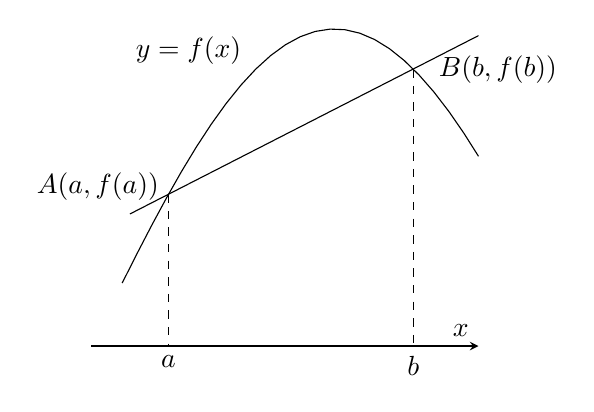
\begin{tikzpicture}
\begin{axis}[clip=false,small,axis lines=middle,xlabel={$x$},xmin=0,ymin=0,xtick={\empty},ytick={\empty},y axis line style={draw=none}]
\addplot[domain=0.2:2.5]{sin(deg(x))}node[pos=0.4,above left]{$y=f(x)$};
\addplot[domain=0.25:2.5]{0.25*x+0.354};
%\draw[] (axis cs:0.49932,0.4788)node[left]{$A$}--(axis cs:2.08,0.873)node[above]{$B$};
\draw[dashed](axis cs:0.49932,0.4788)node[left,yshift={1mm}]{$A(a,f(a))$}--(axis cs:0.49932,0)node[below]{$a$};
\draw[dashed](axis cs:2.08,0.873)node[right,xshift=2mm]{$B(b,f(b))$}--(axis cs:2.08,0)node[below]{$b$};
\end{axis}
\end{tikzpicture}
\caption{وقفہ \عددی{[a,b]} پر \عددی{f} اور قطع \عددی{AB} کے ترسیم۔}
\end{subfigure}\hfill
\begin{subfigure}[t]{0.45\textwidth}
\centering
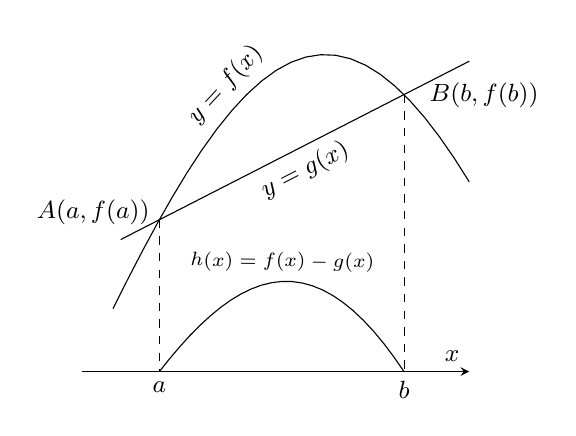
\begin{tikzpicture}[font=\small]
\begin{axis}[clip=false,small,axis lines=middle,xlabel={$x$},xmin=0,ymin=0,xtick={\empty},ytick={\empty},y axis line style={draw=none}]
\addplot[domain=0.2:2.5]{sin(deg(x))}node[pos=0.4,sloped,above]{$y=f(x)$};
\addplot[,domain=0.25:2.5]{0.25*x+0.354}node[pos=0.5,sloped,below]{$y=g(x)$};
\addplot[domain=0.4993:2.08]{sin(deg(x))-0.25*x-0.354}node[pos=0.5,sloped,above,font=\scriptsize]{$h(x)=f(x)-g(x)$};
%\draw[] (axis cs:0.49932,0.4788)node[left]{$A$}--(axis cs:2.08,0.873)node[above]{$B$};
\draw[dashed](axis cs:0.49932,0.4788)node[left,yshift={1mm}]{$A(a,f(a))$}--(axis cs:0.49932,0)node[below]{$a$};
\draw[dashed](axis cs:2.08,0.873)node[right,xshift=2mm]{$B(b,f(b))$}--(axis cs:2.08,0)node[below]{$b$};
\end{axis}
\end{tikzpicture}
\caption{\عددی{f(x)} اور \عددی{g(x)} کے بیچ افقی فاصلہ \عددی{h(x)} ہے۔}
\end{subfigure}
\caption{مسئلہ اوسط قیمت۔}
\label{شکل_مسئلہ_استعمال_اوسط_قیمت}
\end{figure}

تفاعل \عددی{h} وقفہ \عددی{[a,b]} پر مسئلہ رول کو مطمئن کرتا ہے۔ تفاعل \عددی{h} وقفہ \عددی{[a,b]} پر استمراری اور \عددی{(a,b)} پر قابل تفرق  ہے (چونکہ اس وقفہ پر \عددی{f} اور \عددی{g} استمراری اور قابل تفرق ہیں)۔ مزید چونکہ \عددی{f} اور \عددی{g} دونوں نقطہ \عددی{A} اور \عددی{B} سے گزرتے ہیں لہٰذا \عددی{h(a)=h(b)=0} ہے۔ یوں \عددی{(a,b)} میں کسی نقطہ \عددی{c} پر \عددی{h'(x)=0} ہو گا۔ یہ وہ نقطہ ہے جو ہمیں مساوات \حوالہ{مساوات_استعمال_مسئلہ_اوسط_قیمت_الف} میں درکار ہے۔

مساوات \حوالہ{مساوات_استعمال_مسئلہ_اوسط_قیمت_الف} کی تصدیق کی خاطر ہم \عددی{x} کے لحاظ سے مساوات \حوالہ{مساوات_استعمال_مسئلہ_اوسط_قیمت_ج} کے دونوں ہاتھ  کا تفرق لے کر اس میں \عددی{x=c} پر کرتے ہیں۔
\begin{align*}
h'(x)&=f'(x)-\frac{f(b)-f(a)}{b-a}&&\text{\RL{(تفرق)}}\\
h'(c)&=f'(c)-\frac{f(b)-f(a)}{b-a}&& (x=c)\\
0&=f'(c)-\frac{f(b)-f(a)}{b-a}&&(h'(c)=0)\\
f'(c)&=\frac{f(b)-f(a)}{b-a}
\end{align*}
یوں ثبوت مکمل ہوتا ہے۔
\انتہا{ثبوت}
%===============================

دھیان رہے کہ مسئلہ اوسط قیمت میں نقطہ \عددی{a} یا \عددی{b} پر \عددی{f} کا قابل تفرق ہونا ضروری نہیں ہے البتہ ان نقطوں پر \عددی{f} کا استمراری ہونا کافی ہے (شکل \حوالہ{شکل_استعمال_تفرق_ضروری_نہیں})۔
\begin{figure}
\centering
\begin{minipage}{0.45\textwidth}
\centering
\begin{tikzpicture}
\begin{axis}[clip=false,axis equal,small,axis lines=middle,xlabel={$x$},ylabel={y},xtick={-1,1},ytick={1},ymax=1.5,xmin=-1.25,xmax=1.5,ylabel style={at={(current axis.above origin)},anchor=south}]
\addplot[domain=-1:-0.9]{sqrt(1-x^2)};
\addplot[domain=0.9:1]{sqrt(1-x^2)};
\addplot[domain=-0.9:0.9]{sqrt(1-x^2)}node[pos=0.5,above right,align=center]{$y=\sqrt{1-x^2}$ \\   $-1\le x\le 1$};
\addplot[] plot coordinates {(-0.5,1) (0.5,1)};
\end{axis}
\end{tikzpicture}
\caption{
اگرچہ \عددی{y=\sqrt{1-x^2}} نقطہ \عددی{-1} اور \عددی{1} پر نا قابل تفرق ہے یہ \عددی{[-1,1]} پر مسئلہ اوسط قیمت کو مطمئن کرتا ہے۔
}
\label{شکل_استعمال_تفرق_ضروری_نہیں}
\end{minipage}\hfill
\begin{minipage}{0.45\textwidth}
\centering
\begin{tikzpicture}
\begin{axis}[clip=false,axis equal,small,axis lines=middle,xlabel={$x$},ylabel={y},xtick={1,2},ytick={1,4},ylabel style={at={(current axis.above origin)},anchor=south},ymin=-0.2,ymax=5]
\addplot[domain=0:2]{x^2}node[pos=0.7,right]{$y=x^2$};
\addplot[domain=0.7:1.5]{2*x-1};
\draw(axis cs:0,0) node[below left]{$A(0,0)$}--(axis cs:2,4)node[above]{$B(2,4)$};
\draw(axis cs:0,0)node[circ]{} (axis cs:1,1)node[circ]{}node[right]{$(1,1)$}  (axis cs:2,4)node[circ]{};
\end{axis}
\end{tikzpicture}
\caption{نقطہ \عددی{c=1} پر مماس قطع \عددی{AB} کے متوازی ہے (مثال \حوالہ{مثال_استعمال_یہاں_نقطہ_دیکھ_سکتے_ہیں})}
\label{شکل_مثال_استعمال_یہاں_نقطہ_دیکھ_سکتے_ہیں}
\end{minipage}
\end{figure}
 ہم عموماً \عددی{c} کے بارے میں صرف اتنا ہی جانتے ہیں جتنا یہ مسئلہ ہمیں بتاتا ہے، یعنی کہ، \عددی{c} موجود ہے۔اگلی مثال کی طرح بعض اوقات ہم \عددی{c} کو جان پاتے ہیں لیکن ایسا شاذونادر ہو گا۔

\ابتدا{مثال}\شناخت{مثال_استعمال_یہاں_نقطہ_دیکھ_سکتے_ہیں}
وقفہ \عددی{0\le x\le 2} پر تفاعل \عددی{f(x)=x^2} استمراری ہے اور \عددی{0<x<2} پر یہ قابل تفرق ہے (شکل \حوالہ{شکل_مثال_استعمال_یہاں_نقطہ_دیکھ_سکتے_ہیں})۔ چونکہ \عددی{f(0)=0} اور \عددی{f(2)=4} ہیں لہٰذا مسئلہ اوسط قیمت کے تحت اس وقفہ میں نقطہ \عددی{c} پر تفرق \عددی{f'(x)=2x} کی قیمت لازماً \عددی{\tfrac{4-0}{2-0}=2} ہو گی۔ موجودہ مثال میں ہم \عددی{2x=2} کو حل کرتے ہوئے
 \عددی{x=c=1} حاصل کر پاتے ہیں۔ 
\انتہا{مثال}
%=======================

\جزوحصہء{طبعی تشریح}
اگر ہم \عددی{[a,b]} پر \عددی{\tfrac{f(b)-f(a)}{b-a}} کو \عددی{f} کی  اوسط تبدیلی اور \عددی{f'(c)} کو لمحاتی تبدیلی تصور کریں تب مسئلہ اوسط قیمت کہتا ہے کہ کسی اندرونی   نقطہ پر لمحاتی تبدیلی ضرور پورے وقفہ پر اوسط تبدیلی کے برابر ہو گی۔

\ابتدا{مثال}
ایک گاڑی ساکن حال سے شروع ہر کر \عددی{8} سیکنڈوں میں کل \عددی{120} میٹر فاصلہ طے کرتی ہے۔ان \عددی{8} سیکنڈوں کے لئے گاڑی کی اوسط رفتار \عددی{\tfrac{120}{8}=\SI{15}{\meter\per\second}} ہے۔ مسئلہ اوسط قیمت کہتا ہے کہ ان آٹھ سیکنڈوں میں کسی لمحہ رفتار پیما ٹھیک یہی رفتار دکھائے گا۔
\انتہا{مثال}
%=======================


\جزوحصہء{نتائج صریح اور چند جوابات}
اس حصہ کے شروع میں ہم نے پوچھا کہ کس تفاعل کا تفرق صفر ہو گا۔مسئلہ اوسط قیمت کا پہلا نتیجہ صریح اس کا جواب دیتا ہے۔

\ابتدا{نتیجہ صریح}\شناخت{نتیجہ_صریح_استعمال_پہلا}\موٹا{صفر تفرق کے تفاعل مستقل ہوں گے}\\
اگر وقفہ \عددی{I} کے ہر نقطہ پر \عددی{f'(x)=0} ہو تب \عددی{I} میں تمام \عددی{x} پر \عددی{f(x)=C} ہو گا جہاں \عددی{C} مستقل ہے۔
\انتہا{نتیجہ صریح}
%=======================

ہم جانتے ہیں کہ اگر وقفہ \عددی{I} پر تفاعل \عددی{f} کی قیمت مستقل ہو تب \عددی{I} پر \عددی{f} قابل تفرق ہو گا اور \عددی{I} میں تمام \عددی{x} پر \عددی{f'(x)=0} ہو گا۔ نتیجہ صریح اس کا الٹ پیش کرتا ہے۔

%=================
\ابتدا{ثبوت نتیجہ صریح}
ہم دکھانا چاہتے ہیں کہ \عددی{I} پر \عددی{f} کی قیمت مستقل ہے۔ہم \عددی{I} میں ہر دو نقطوں \عددی{x_1} اور \عددی{x_2} پر \عددی{f(x_1)=f(x_2)} دکھاتے ہوئے ایسا کرتے ہیں۔

فرض کریں \عددی{x_1} اور \عددی{x_2} وقفہ \عددی{I} میں کوئی بھی دو نقطے ہیں جن کی شمار بائیں سے دائیں جانب ہے لہٰذا \عددی{x_1<x_2} ہو گا۔یوں \عددی{[x_1,x_2]} پر \عددی{f} مسئلہ اوسط قیمت کو مطمئن کرے گا۔ یہ \عددی{} کے ہر نقطہ پر قابل تفرق ہو گا لہٰذا یہ ہر اس نقطہ پر استمراری بھی ہو گا۔یوں \عددی{x_1} اور \عددی{x_2} کے بیچ کسی نقطہ \عددی{c} پر
\begin{align*}
\frac{f(x_2)-f(x_1)}{x_2-x_1}=f'(c)
\end{align*}
ہو گا۔چونکہ پورے \عددی{I} پر \عددی{f'=0} ہے لہٰذا اس مساوات کو درج ذیل لکھا جا سکتا ہے۔
\begin{align*}
\frac{f(x_2)-f(x_1)}{x_2-x_1}=f'(c),\quad f(x_2)-f(x_1)=0,\quad f(x_1)=f(x_2)
\end{align*}
\انتہا{ثبوت نتیجہ صریح}
%==========================

اس حصہ کے شروع میں ہم نے یہ بھی پوچھا کہ کیا ہم اسراع سے پیچھے کی طرف چلتے ہوئے رفتار اور ہٹاو تلاش کر سکتے ہیں۔یہ کا جواب اگلا نتیجہ صریح پیش کرتا ہے۔

\ابتدا{نتیجہ صریح}\شناخت{نتیجہ_صریح_استعمال_دوم}\موٹا{ایک جیسے تفرق والے تفاعل میں مستقل کا فرق ہو گا}\\
اگر وقفہ \عددی{I} کے ہر نقطہ پر \عددی{f'(x)=g'(x)} ہو تب ایسا مستقل \عددی{C} موجود ہو گا کہ \عددی{I} میں تمام \عددی{x} پر \عددی{f(x)=g(x)+C} ہو۔ 
\انتہا{نتیجہ صریح}
%===================
\ابتدا{ثبوت نتیجہ صریح}
\عددی{I} میں ہر نقطہ پر تفاعل فرق \عددی{h=f-g} کا تفرق
\begin{align*}
h'(x)=f'(x)-h'(x)=0
\end{align*}
ہو گا۔یوں  نتیجہ صریح \حوالہ{نتیجہ_صریح_استعمال_پہلا} کے تحت \عددی{I} پر \عددی{h(x)=C} ہو گا۔یوں \عددی{f(x)-g(x)=C} یا \عددی{f(x)=g(x)+C} ہو گا۔
\انتہا{ثبوت نتیجہ صریح}
%=======================

نتیجہ صریح \حوالہ{نتیجہ_صریح_استعمال_دوم} کہتا ہے  کہ وقفہ پر دو تفاعل کے فرق کا تفرق صرف اس صورت صفر کے برابر ہو گا جب اس وقفہ پر ان تفاعل کا مستقل فرق ہو۔ مثال کے طور پر ہم جانتے ہیں کہ \عددی{(-\infty,\infty)} پر \عددی{f(x)=x^2} کا تفرق \عددی{2x} ہے۔ایسا دوسرا تفاعل جس کا \عددی{(-\infty,\infty)} پر تفرق \عددی{2x} ہو کا کلیہ لازماً \عددی{x^2+C} ہو گا (شکل \حوالہ{شکل_نتیجہ_صریح_استعمال_دوم})۔
\begin{figure}
\centering
\begin{minipage}{0.45\textwidth}
\centering
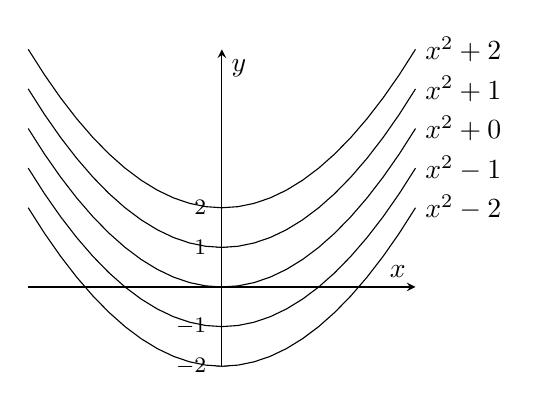
\begin{tikzpicture}
\begin{axis}[clip=false,small,axis lines=middle,xlabel={$x$},ylabel={$y$},ytick={-2,-1,1,2},xtick={\empty}]
\addplot[domain=-2:2]{x^2}node[right]{$x^2+0$};
\addplot[domain=-2:2]{x^2+1}node[right]{$x^2+1$};
\addplot[domain=-2:2]{x^2+2}node[right]{$x^2+2$};
\addplot[domain=-2:2]{x^2-1}node[right]{$x^2-1$};
\addplot[domain=-2:2]{x^2-2}node[right]{$x^2-2$};
\end{axis}
\end{tikzpicture}
\caption{نتیجہ صریح \حوالہ{نتیجہ_صریح_استعمال_دوم} کہتا ہے کہ ایک جیسے تفرق والے تفاعل میں صرف انتصابی فرق پایا جاتا ہے۔}
\label{شکل_نتیجہ_صریح_استعمال_دوم}
\end{minipage}\hfill
\begin{minipage}{0.45\textwidth}
\centering
\begin{tikzpicture}
\begin{axis}[clip=false,small,axis lines=middle,xlabel={$x$},ylabel={$y$},ytick={2,3},xtick={\empty},ymin=-0.25,ymax=3.5]
\addplot[domain=-4.713:4.713,smooth]{3-cos(deg(x))}node[left]{$3-\cos x$};
\end{axis}
\end{tikzpicture}
\caption{ترسیم برائے مثال \حوالہ{مثال_استعمال_نتیجہ_صریح_کوسائن}}
\label{شکل_مثال_استعمال_نتیجہ_صریح_کوسائن}
\end{minipage}
\end{figure}

%=======================
\ابتدا{مثال}\شناخت{مثال_استعمال_نتیجہ_صریح_کوسائن}
ایسا تفاعل \عددی{f(x)} تلاش کریں جس کا تفرق \عددی{\sin x} ہو اور جو نقطہ \عددی{(0,2)} سے گزرتا ہو۔\\
حل:\quad
چونکہ \عددی{g(x)=-\cos x} کا تفرق بھی \عددی{\sin x} ہے لہٰذا \عددی{f(x)=-\cos x +C} ہو گا۔دیا گیا نقطہ اس میں پر کرتے ہوئے مستقل \عددی{C}حاصل کرتے ہیں۔
\begin{align*}
f(0)=-\cos(0)+C=2\quad \implies\quad C=3
\end{align*} 
یوں درکار تفاعل \عددی{f(x)=-\cos x+3} ہے (شکل \حوالہ{شکل_مثال_استعمال_نتیجہ_صریح_کوسائن})۔
\انتہا{مثال}
%==============================
\جزوحصہء{اسراع سے سمتی رفتار اور ہٹاو کا حصول}
سطح زمین کے قریب جہاں \عددی{g=\SI{9.8}{\meter\per\second\squared}} ہے ساکن حال سے آزادانہ گرتے ہوئے جسم کی سمتی رفتار اور ہٹاو تلاش کرتے ہیں۔

ہم جانتے ہیں کہ سمتی رفتار \عددی{v} ایسا تفاعل ہے جس کا تفرق \عددی{9.8} کے برابر ہے۔ ہم یہ جانتے ہیں کہ \عددی{g(t)=9.8 t} کا تفرق \عددی{9.8} ہے لہٰذا نتیجہ صریح \حوالہ{نتیجہ_صریح_استعمال_دوم} کے تحت
\begin{align*}
v(t)=9.8t+C
\end{align*}
ہو گا جہاں \عددی{C} مستقل ہے۔لمحہ \عددی{t=0} پر جسم ساکن ہو گا لہٰذا
\begin{align*}
v(0)=9.8(0)+C\quad \implies \quad C=0 
\end{align*}
ہو گا۔یوں سمتی رفتار تفاعل \عددی{v(t)=9.8 t} ہو گا۔ ہم یہ بھی جانتے ہیں کہ \عددی{h(t)=4.9t^2} کا تفرق \عددی{9.8t} ہے لہٰذا  نتیجہ صریح \حوالہ{نتیجہ_صریح_استعمال_دوم} کے تحت
\begin{align*}
s(t)=4.9t^2+C
\end{align*}
ہو گا جہاں \عددی{C} مستقل ہے۔چونکہ لمحہ \عددی{t=0} پر ہٹاو صفر ہے لہٰذا
\begin{align*}
s(0)=4.9(0^2)+C=0\quad \implies \quad C=0
\end{align*} 
یعنی \عددی{s(t)=4.9t^2} ہو گا۔

کسی تفاعل کی شرح تبدیلی سے تفاعل حاصل کرنے کی صلاحیت، احصاء کی اہم ترین طاقت ہے۔ اس پر مزید بات اگلے باب میں کی جائے گی۔

\جزوحصہء{بڑھتا تفاعل اور گھٹتا تفاعل}
اس حصہ کے شروع میں ہم نے پوچھا کہ کس قسم کے تفاعل کا تفرق مثبت اور کس کا تفرق منفی ہو گا۔مسئلہ اوسط قیمت کا تیسرا نتیجہ صریح جو اس کا جواب دیتا ہے کہتا ہے کہ بڑھتے ہوئے تفاعل کا تفرق مثبت اور گھٹے ہوئے تفاعل کا تفرق منفی ہو گا۔

\ابتدا{تعریف}
فرض کریں وقفہ \عددی{I} پر تفاعل \عددی{f} معین ہے اور اس وقفہ پر \عددی{x_1} اور \عددی{x_2} کوئی بھی دو نقطے ہیں۔
\begin{enumerate}[1.]
\item
اگر \عددی{x_1<x_2} کی صورت میں \عددی{f(x_1)<f(x_2)} ہو تب \عددی{I} پر \عددی{f} \اصطلاح{بڑھتا}\فرہنگ{بڑھتا}\حاشیہب{increasing}\فرہنگ{increasing} تفاعل کہلاتا ہے۔
\item
اگر \عددی{x_1<x_2} کی صورت میں \عددی{f(x_1)>f(x_2)} ہو تب \عددی{I} پر \عددی{f} \اصطلاح{گھٹتا}\فرہنگ{گھٹتا}\حاشیہب{decreasing}\فرہنگ{decreasing} تفاعل کہلاتا  ہے۔
\end{enumerate}
\انتہا{تعریف}
%=====================

\ابتدا{نتیجہ صریح}\شناخت{نتیجہ_صریح_استعمال_سوم}\موٹا{بڑھتے اور گھٹتے تفاعل کا پہلا تفرقی پرکھ}\\
فرض کریں \عددی{[a,b]} پر \عددی{f} استمراری  اور \عددی{(a,b)} پر \عددی{f} قابل تفرق ہے۔
\begin{itemize}
\item
اگر \عددی{(a,b)} کے ہر نقطہ پر \عددی{f'>0} ہو تب \عددی{[a,b]} پر \عددی{f} بڑھتا ہے۔
\item
اگر \عددی{(a,b)} کے ہر نقطہ پر \عددی{f'<0} ہو تب \عددی{[a,b]} پر \عددی{f} گھٹتا ہے۔
\end{itemize}
\انتہا{نتیجہ صریح}
%==============================
\ابتدا{ثبوت نتیجہ صریح}
فرض کریں \عددی{[a,b]} میں \عددی{x_1} اور \عددی{x_2} کوئی دو نقطے ہیں جہاں \عددی{x_1<x_2} ہے۔ وقفہ \عددی{[x_1,x_2]} پر مسئلہ اوسط قیمت تفاعل \عددی{f} کے لئے کہتا ہے کہ
\begin{align}\label{مساوات_استعمال_نتیجہ_صریح_سوم_الف}
f(x_2)-f(x_1)=f'(c)(x_2-x_1)
\end{align}
ہو گا جہاں \عددی{x_1} اور \عددی{x_2} کے بیچ \عددی{c} ایک موزوں نقطہ ہے۔ چونکہ \عددی{x_2-x_1} مثبت قیمت ہے لہٰذا مساوات \حوالہ{مساوات_استعمال_نتیجہ_صریح_سوم_الف} کے دائیں ہاتھ کی علامت وہی ہو گی جو \عددی{f'(c)} کی ہے۔یوں \عددی{(a,b)} پر مثبت \عددی{f'(c)} کی صورت میں \عددی{f(x_2)>f(x_1)} ہو گا جبکہ \عددی{(a,b)} پر منفی \عددی{f'(c)} کی صورت میں \عددی{f(x_1)<f(x_2)} ہو گا۔
\انتہا{ثبوت نتیجہ صریح}
%==============================

\ابتدا{مثال}\شناخت{مثال_استعمال_بڑھتا_گھٹتا}
وقفہ \عددی{(-\infty,0)} پر تفاعل \عددی{f(x)=x^2} کا تفرق \عددی{f'(x)=2x<0} ہے لہٰذا اس وقفے پر \عددی{f} گھٹے گا۔ وقفہ \عددی{(0,\infty)} پر تفاعل \عددی{f(x)=x^2} کا تفرق \عددی{f'(x)=2x>0} ہے لہٰذا اس وقفے پر \عددی{f} بڑھے گا (شکل \حوالہ{شکل_مثال_استعمال_بڑھتا_گھٹتا})۔
\begin{figure}
\centering
\begin{tikzpicture}[font=\small]
\begin{axis}[clip=false,small,axis lines=middle,xlabel={$x$},ylabel={$y$},xtick={-2,-1,1,2},ytick={1,2,3,4},xmin=-2.5,xmax=2.5,ymax=4.9]
\addplot[domain=-2:2]{x^2}node[left]{$y=x^2$}node[pos=0.15,below left,align=center]{\RL{گھٹتا تفاعل}\\  $y'<0$}node[pos=0.85,below right,align=center]{\RL{بڑھتا تفاعل}\\  $y'>0$}node[pos=0.5,pin=-45:{$y'=0$}]{};
\end{axis}
\end{tikzpicture}
\caption{ترسیم برائے مثال \حوالہ{مثال_استعمال_بڑھتا_گھٹتا}}
\label{شکل_مثال_استعمال_بڑھتا_گھٹتا}
\end{figure}
\انتہا{مثال}
%==================

\حصہء{سوالات}
\موٹا{مسئلہ اوسط قیمت میں \عددی{c} کی تلاش}\\
سوال \حوالہ{سوال_استعمال_موزوں_الف} تا سوال \حوالہ{سوال_استعمال_موزوں_ب} میں دیے وقفہ اور تفاعل کے لئے  \عددی{c} کی ایسی قیمت  تلاش کریں جو مسئلہ اوسط قیمت کے نتیجہ 
\begin{align*}
\frac{f(b)-f(a)}{b-a}=f'(c)
\end{align*}
کو مطمئن کرتی ہو۔

\ابتدا{سوال}\شناخت{سوال_استعمال_موزوں_الف}
$f(x)=x^2+2x-1,\quad [0,1]$\\
جواب:\quad
$\tfrac{1}{2}$
\انتہا{سوال}
%=======================
\ابتدا{سوال}
$f(x)=x^{2/3},\quad [0,1]$
\انتہا{سوال}
%========================
\ابتدا{سوال}
$f(x)=x+\tfrac{1}{x},\quad [\tfrac{1}{2},2]$\\
جواب:\quad
$1$
\انتہا{سوال}
%========================
\ابتدا{سوال}\شناخت{سوال_استعمال_موزوں_ب}
$f(x)=\sqrt{x-1},\quad [1,3]$
\انتہا{سوال}
%========================
\موٹا{قیاس کی پرکھ اور استعمال}\\
سوال \حوالہ{سوال_استعمال_قیاس_الف} تا سوال \حوالہ{سوال_استعمال_قیاس_ب} میں کون سے تفاعل دیے وقفہ پر مسئلہ اوسط قیمت کے قیاس کو مطمئن کرتے ہیں اور کون سے تفاعل ایسا نہیں کرتے ہیں۔ اپنے جواب کی وجہ پیش کریں۔ 

\ابتدا{سوال}\شناخت{سوال_استعمال_قیاس_الف}
$f(x)=x^{2/3},\quad [-1,8]$\\
جواب:\quad
نہیں کرتا؛ دائرہ کار کے اندرونی نقطہ \عددی{x=0} پر \عددی{f} نا قبل تفرق ہے۔ 
\انتہا{سوال}
%==========================
\ابتدا{سوال}
$f(x)=x^{4/5},\quad [0,1]$
\انتہا{سوال}
%===========================
\ابتدا{سوال}
$f(x)=\sqrt{x(1-x)},\quad [0,1]$\\
جواب:\quad
کرتا ہے۔
\انتہا{سوال}
%===========================
\ابتدا{سوال}\شناخت{سوال_استعمال_قیاس_ب}
$f(x)=\begin{cases} \tfrac{\sin x}{x},&-\pi\le x< 0\\ 0,&x=0 \end{cases}$
\انتہا{سوال}
%===========================
\ابتدا{سوال}
درج ذیل تفاعل \عددی{x=0} اور \عددی{x=1} پر صفر کے برابر ہے اور \عددی{(0,1)} پر قابل تفرق ہے لیکن \عددی{(a,b)} پر اس کا تفرق کبھی بھی صفر نہیں ہے۔ 
\begin{align*}
f(x)=\begin{cases} x,& 0\le x<1\\ 0,&x=1 \end{cases}
\end{align*}
ایسا کیوں ممکن ہے؟ کیا مسئلہ رول نہیں کہتا کہ \عددی{(0,1)} پر کہیں تفرق صفر ہو گا؟ اپنے جواب کی وجہ پیش کریں۔
\انتہا{سوال}
%====================
\ابتدا{سوال}
وقفہ \عددی{[0,2]} پر \عددی{a}، \عددی{m} اور \عددی{b} کی کون سی قیمتوں کے لئے  درج ذیل تفاعل مسئلہ اوسط قیمت کی قیاس کو مطمئن کرتا ہے؟
\begin{align*}
f(x)=\begin{cases} 3,&x=0\\ -x^2+3x+a,&0<x<1\\ mx+b,&1\le x\le 2  \end{cases}
\end{align*}
\انتہا{سوال}
%======================
\موٹا{جذر (صفر)}

\ابتدا{سوال}\شناخت{سوال_استعمال_جذر_الف}

\begin{enumerate}[a.]
\item
باری باری درج ذیل کثیر رکنیوں کے صفر کو ایک لکیر پر ترسیم کریں۔ساتھ ہی ان کے یک درجی تفرق کے  صفر بھی ترسیم کریں۔
\begin{enumerate}[1.]
\item
$y=x^2-4$
\item
$y=x^2+8x+15$
\item
$y=x^3-3x^2+4=(x+1)(x-2)^2$
\item
$y=x^3-33x^2+216x=x(x-9)(x-24)$
\end{enumerate}
\item
مسئلہ رول کی مدد سے ثابت کریں کہ 
$x^n+a_{n-1}x^{n-1}+\cdots+a_1x+a_0$
کے ہر دو صفر کے بیچ \\
$nx^{n-1}+(n-1)a_{n-1}x^{n-2}+\cdots+a_1$
کا ایک صفر پایا جاتا ہے۔
\end{enumerate}
جواب:\quad 
(ا) شکل \حوالہ{شکل_سوال_استعمال_جذر_الف}
\begin{figure}
\centering
\begin{tikzpicture}
\draw[-latex](0,0)node[left]{$(1)$}--++(7,0)node[right]{$x$};
\draw[-latex](0,-1)node[left]{$(2)$}--++(7,0)node[right]{$x$};
\draw[-latex](0,-2)node[left]{$(3)$}--++(7,0)node[right]{$x$};
\foreach \x/\s in {3/-2,4/0,5/2}{\draw(\x,0)node[circ]{}node[below]{$\s$}--++(0,0.1);}
\foreach \x/\s in {3/-5,4/-4,5/-3}{\draw(\x,-1)node[circ]{}node[below]{$\s$}--++(0,0.1);}
\foreach \x/\s in {1/0,2/4,3/9,5/18,6/24}{\draw(\x,-2)node[circ]{}node[below]{$\s$}--++(0,0.1);}
\end{tikzpicture}
\caption{حل ترسیم سوال \حوالہ{سوال_استعمال_جذر_الف}}
\label{شکل_سوال_استعمال_جذر_الف}
\end{figure}
\انتہا{سوال}
%=====================
\ابتدا{سوال}
فرض کریں کہ وقفہ \عددی{[a,b]} میں \عددی{f'''} استمراری ہے اور اس وقفہ پر \عددی{f} کے تین صفر پائے جاتے ہیں۔دکھائیں کہ اس وقفہ پر \عددی{f''} کا کم سے کم ایک صفر پایا جائے گا۔ اس نتیجہ کو عمومی بنائیں۔
\انتہا{سوال}
%=========================
\ابتدا{سوال}
دکھائیں کہ اگر پورے \عددی{[a,b]} پر \عددی{f''>0}  ہو تب \عددی{[a,b]} میں \عددی{f'} کا زیادہ سے زیادہ ایک صفر پایا جائے گا۔اگر \عددی{[a,b]} پر \عددی{f''<0} ہو تب کیا ہو گا؟
\انتہا{سوال}
%=====================
\ابتدا{سوال}
دکھائیں کہ کعبی کثیر رکنی کے صفروں کی زیادہ سے زیادہ تعداد تین ممکن ہے۔
\انتہا{سوال}
%================================

\موٹا{نظریہ اور مثالیں}\\
\ابتدا{سوال}
دکھائیں کہ دو گھنٹوں کی صفر میں کسی لمحہ پر گاڑی کا رفتار پیما ضرور دو گھنٹوں کی اوسط رفتار دکھائے گا۔
\انتہا{سوال}
%====================
\ابتدا{سوال}\ترچھا{تبدیلی درجہ حرارت}\quad
برف سے حرارت پیما کو نکال کر ابلتے  ہوئے پانی میں رکھنے سے اس کا درجہ حرارت \عددی{14} سیکنڈوں میں \عددی{\SI{-19}{\celsius}} سے بڑھ کر \عددی{\SI{100}{\celsius}} ہوتا ہے۔ دکھائیں کہ اس دوران درجہ حرارت میں تبدیلی کی شرح کسی لمحے پر \عددی{\SI{8.5}{\celsius\per\second}} ضرور ہو گی۔ 
\انتہا{سوال}
%====================
\ابتدا{سوال}
فرض کریں کہ وقفہ \عددی{[0,1]} پر قابل تفرق تفاعل \عددی{f} کا تفرق کبھی صفر نہیں ہوتا ہے۔دکھائیں کہ \عددی{f(0\ne f(1)} ہو گا۔ 
\انتہا{سوال}
%===================
\ابتدا{سوال}
دکھائیں کہ \عددی{a} اور \عددی{b} کی کسی بھی قیمتوں کے لئے \عددی{\abs{\sin b-\sin a}\le\abs{b-a}} ہو گا۔
\انتہا{سوال}
%======================
\ابتدا{سوال}
فرض کریں \عددی{[a,b]} پر \عددی{f} قابل تفرق ہے اور \عددی{f(b)<f(a)} ہے۔ کیا \عددی{[a,b]} پر \عددی{f'} کی قیمت کے بارے میں کچھ کہنا ممکن ہو گا؟
\انتہا{سوال}
%=========================
\ابتدا{سوال}
فرض کریں \عددی{[a,b]} پر \عددی{f} اور \عددی{g} قابل تفرق ہیں اور \عددی{f(a)=g(a)} اور \عددی{f(b)=g(b)} ہیں۔دکھائیں کہ \عددی{a} اور \عددی{b} کے بیچ کم سے کم ایسا ایک نقطہ پایا جاتا ہے جہاں \عددی{f} اور \عددی{g} کی ترسیمات کے مماس آپس میں متوازی ہیں۔
\انتہا{سوال}
%==========================
\ابتدا{سوال}
فرض کریں \عددی{x} کی ہر قیمت کے لئے \عددی{f} قابل تفرق ہے۔مزید فرض کریں کہ \عددی{f(1)=1} ہے اور  \عددی{(-\infty,1)} پر  \عددی{f'<0} ہے اور \عددی{(1,\infty)} پر \عددی{f'>0} ہے۔
\begin{enumerate}[a.]
\item
دکھائیں کہ تمام \عددی{x} پر \عددی{f(x)\ge 1} ہو گا۔
\item
کیا \عددی{f'(1)=0} لازماً ہو گا؟ وجہ پیش کریں۔

\end{enumerate}
\انتہا{سوال}
%===========================
\ابتدا{سوال}
فرض کریں \عددی{f(x)=px^2+qx+r} بند وقفہ \عددی{[a,b]} پر معین ہے۔دکھائیں کہ \عددی{(a,b)} میں ٹھیک ایک نقطہ \عددی{c} پر \عددی{f} مسئلہ اوسط قیمت  کے نتیجہ پر پورا اترتا ہے۔ 
\انتہا{سوال}
%============================
\ابتدا{سوال}\ترچھا{حیرت کن ترسیم}\quad
درج ذیل تفاعل ترسیم کریں۔
\begin{align*}
f(x)=\sin x\sin(x+2)-\sin^2(x+1)
\end{align*}
یہ ترسیم کیا کرتی ہے؟ یہ تفاعل اس طرح کا رویہ کیوں رکھتا ہے؟ اپنے جواب کی وجہ پیش کریں۔
\انتہا{سوال}
%=========================
\ابتدا{سوال}
اگر دو تفاعل \عددی{f(x)} اور \عددی{g(x)} کی ترسیمات مستوی میں ایک ہی نقطہ سے شروع ہوتے ہوں اور ہر نقطہ پر ان کی شرح تبدیلی ایک جیسی ہو تب کیا یہ تفاعل بالکل ایک جیسے نہیں ہوں گے؟ اپنے جواب کہ وجہ پیش کریں۔ 
\انتہا{سوال}
%=======================
\ابتدا{سوال}
\begin{enumerate}[a.]
\item
دکھائیں کہ تفاعل \عددی{g(x)=\tfrac{1}{x}} اپنے دائرہ کار کے ہر وقفہ میں گھٹتا ہے۔
\item
اگر جزو (ا) کا نتیجہ درست ہو تب \عددی{g(1)=1} کس طرح \عددی{g(-1)=-1} سے بڑا ہو سکتا ہے؟
\end{enumerate}
\انتہا{سوال}
%=========================
\ابتدا{سوال}\شناخت{سوال_استعمال_مسئلہ_اوسط_قیمت_الف}
فرض کریں وقفہ \عددی{[a,b]} میں تفاعل \عددی{f} معین ہے۔ درج ذیل کو مطمئن کرنے کی خاطر \عددی{f} پر کون سے شرائط لاگو کرنے ہوں گے
\begin{align*}
f'\,\text{\RL{کم سے کم}}\le \frac{f(b)-f(a)}{b-a}\le f'\,\text{\RL{زیادہ سے زیادہ}}
\end{align*} 
جہاں کم سے کم \عددی{f'} اور زیادہ سے زیادہ \عددی{f'} سے مراد \عددی{[a,b]} پر بالترتیب \عددی{f'} کی  کم سے کم اور زیادہ سے زیادہ قیمت ہے۔
\انتہا{سوال}
%=================
\ابتدا{سوال}
اگر \عددی{0\le x\le 0.1} پر \عددی{f'(x)=1/(1+x^4\cos x)} ہو اور \عددی{f(0)=1} ہو تب سوال \حوالہ{سوال_استعمال_مسئلہ_اوسط_قیمت_الف} کی عدم مساوات استعمال کرتے ہوئے  \عددی{f(0.1)} کی تخمینی قیمت تلاش کریں۔\\
جواب:\quad
$1.09999\le f(0.1)\le 1.1$
\انتہا{سوال}
%===================
\ابتدا{سوال}
اگر \عددی{0\le x\le 0.1} پر \عددی{f'(x)=1/(1-x^4)} ہو اور \عددی{f(0)=2} ہو تب سوال \حوالہ{سوال_استعمال_مسئلہ_اوسط_قیمت_الف} کی عدم مساوات استعمال کرتے ہوئے  \عددی{f(0.1)} کی تخمینی قیمت تلاش کریں۔
\انتہا{سوال}
%===================
\ابتدا{سوال}\ترچھا{ہندسی اوسط۔} \quad
دو مثبت اعداد \عددی{a} اور \عددی{b} کی \اصطلاح{ہندسی اوسط}\فرہنگ{اوسط!ہندسی}\حاشیہب{geometric mean}\فرہنگ{mean!geometric} سے مراد عدد \عددی{\sqrt{ab}} ہے۔دکھائیں کہ  مسئلہ اوسط قیمت کے نتیجہ میں مثبت اعداد کے وقفہ \عددی{[a,b]}  پر تفاعل \عددی{f(x)=\tfrac{1}{x}} کے لئے \عددی{c} کی قیمت \عددی{\sqrt{ab}} ہے۔ 
\انتہا{سوال}
%=======================
\ابتدا{سوال}\ترچھا{حسابی اوسط۔}\quad
دو اعداد \عددی{a} اور \عددی{b} کی \اصطلاح{حسابی اوسط}\فرہنگ{اوسط!حسابی}\حاشیہب{arithmetic mean}\فرہنگ{mean!arithmetic} \عددی{\tfrac{a+b}{2}} ہے۔ دکھائیں کہ مسئلہ اوسط قیمت میں وقفہ \عددی{[a,b]} پر تفاعل \عددی{f(x)=x^2} کے لئے \عددی{c} کی قیمت \عددی{\tfrac{a+b}{2}} ہو گی۔
\انتہا{سوال}
%=========================
\موٹا{تفرق سے تفاعل کا حصول}\\
\ابتدا{سوال}
فرض کریں \عددی{f(-1)=3} اور تمام \عددی{x} کے لئے \عددی{f'(x)=0} ہے۔ کیا تمام \عددی{x} کے لئے \عددی{f(x)=3} ہو گا؟ اپنے جواب کی وجہ پیش کریں۔\\
جواب:\quad 
ہاں
\انتہا{سوال}
%===================
\ابتدا{سوال}
فرض کریں \عددی{f(0)=5} اور تمام \عددی{x} کے لئے \عددی{f'(x)=2} ہیں۔ کیا تمام \عددی{x} کے لئے \عددی{f(x)=2x+5} ہو گا؟ اپنے جواب کی وجہ پیش کریں۔
\انتہا{سوال}
%=====================
\ابتدا{سوال}
فرض کریں تمام \عددی{x} کے لئے \عددی{f'(0)=2x} ہے۔ درج ذیل صورتوں میں \عددی{f(2)} تلاش کریں۔
\begin{multicols}{3}
\begin{enumerate}[a.]
\item
$f(0)=0$
\item
$f(1)=0$
\item
$f(-2)=3$
\end{enumerate}
\end{multicols}
جواب:\quad
(ا) \عددی{4}، (ب) \عددی{3}، (ج) \عددی{3}
\انتہا{سوال}
%========================
\ابتدا{سوال}
جن تفاعل کا تفرق مستقل ہو ان کے بارے میں کیا کہا جا سکتا ہے؟ اپنے جواب کی وجہ پیش کریں۔
\انتہا{سوال}
%=========================
سوال \حوالہ{سوال_استعمال_تفرق_سے_تفاعل_الف}  تا سوال \حوالہ{سوال_استعمال_تفرق_سے_تفاعل_ب} میں وہ تفاعل تلاش کریں جس کا تفرق دیا گیا ہے۔

\ابتدا{سوال}\شناخت{سوال_استعمال_تفرق_سے_تفاعل_الف}
(ا) \عددی{y'=x}، (ب) \عددی{y'=x^2}، (ج) \عددی{y'=x^3}\\
جواب:\quad
(ا) \عددی{\tfrac{x^2}{2}+C}، (ب) \عددی{\tfrac{x^3}{3}+C}، (ج) \عددی{\tfrac{x^4}{4}+C}
\انتہا{سوال}
%=========================
\ابتدا{سوال}
(ا) \عددی{y'=2x}، (ب) \عددی{y'=2x-1}، (ج) \عددی{y'=3x^2+2x-1}
\انتہا{سوال}
%======================
\ابتدا{سوال}
(ا) \عددی{y'=-\tfrac{1}{x^2}}، (ب) \عددی{y'=1-\tfrac{1}{x^2}}، (ج) \عددی{y'=5+\tfrac{1}{x^2}}\\
جواب:\quad
(ا) \عددی{\tfrac{1}{x}+C}، (ب) \عددی{x+\tfrac{1}{x}+C}، (ج) \عددی{5x-\tfrac{1}{x}+C}
\انتہا{سوال}
%==========================
\ابتدا{سوال}
(ا) \عددی{y'=\tfrac{1}{2\sqrt{x}}}، (ب) \عددی{y'=\tfrac{1}{\sqrt{x}}}، (ج) \عددی{y'=4x-\tfrac{1}{\sqrt{x}}}
\انتہا{سوال}
%==========================
\ابتدا{سوال}
(ا) \عددی{y'=\sin 2t}، (ب) \عددی{y'=\cos \tfrac{t}{2}}، (ج) \عددی{y'=\sin 2t+\cos \tfrac{t}{2}}\\
جواب:\quad
(ا) \عددی{-\tfrac{1}{2}\cos 2t+C}، (ب) \عددی{2\sin\tfrac{t}{2}+C}، (ج) \عددی{-\tfrac{1}{2}\cos 2t+2\sin\tfrac{t}{2}+C}
\انتہا{سوال}
%===========================
\ابتدا{سوال}\شناخت{سوال_استعمال_تفرق_سے_تفاعل_ب}
(ا) \عددی{y'=\sec^2 \theta}، (ب) \عددی{y'=\sqrt{\theta}}، (ج) \عددی{y'=\sqrt{\theta}-\sec^2\theta}
\انتہا{سوال}
%=========================
سوال \حوالہ{سوال_استعمال_تفرق_نقطہ_الف} تا سوال \حوالہ{سوال_استعمال_تفرق_نقطہ_ب} میں وہ تفاعل تلاش کریں جس کا تفرق دیا گیا ہے اور جو دیے گئے  نقطہ سے گزرتا ہے۔

\ابتدا{سوال}\شناخت{سوال_استعمال_تفرق_نقطہ_الف}
$f'(x)=2x-1,\quad N(0,0)$\\
جواب:\quad
$f(x)=x^2-x$
\انتہا{سوال}
%====================
\ابتدا{سوال}
$g'(x)=\tfrac{1}{x^2}+2x,\quad N(-1,1)$
\انتہا{سوال}
%====================
\ابتدا{سوال}
$r'(\theta)=8-\csc^2\theta,\quad N(\tfrac{\pi}{4},0)$\\
جواب:\quad
$r(\theta)=8\theta+\cot \theta-2\pi-1$
\انتہا{سوال}
%========================
\ابتدا{سوال}\شناخت{سوال_استعمال_تفرق_نقطہ_ب}
$r'(t)=\sec t\tan t-1,\quad N(0,0)$
\انتہا{سوال}
%===========================
\موٹا{صفروں  کی گنتی}\\
مساوات \عددی{f(x)=0} کو اعدادی طریقہ سے حل کرنے سے پہلے ہم عموماً  مطلوبہ وقفہ پر  مساوات کی متوقع صفروں کی تعداد جاننا چاہتے ہیں۔ بعض اوقات نتیجہ صریح \حوالہ{نتیجہ_صریح_استعمال_سوم} کی مدد سے ایسا کرنا ممکن ہو گا۔

درج ذیل فرض کریں۔
\begin{enumerate}[1.]
\item
\عددی{[a,b]} پر \عددی{f} استمراری اور \عددی{(a,b)} پر قابل تفرق ہے۔
\item
\عددی{f(a)} اور \عددی{f(b)} کی علامتیں ایک دوسرے کی الٹ ہیں۔
\item
پورے \عددی{(a,b)} پر \عددی{f'>0} اور یا پورے \عددی{(a,b)} پر \عددی{f'<0} ہے۔
\end{enumerate}
تب \عددی{a} اور \عددی{b} کے بیچ \عددی{f} کا ٹھیک ایک صفر پایا جائے گا۔چونکہ یہ پورے \عددی{[a,b]} پر بڑھ رہا ہے اور یا  پورے \عددی{[a,b]} پر گھٹ رہا ہے لہٰذا یہ \عددی{x} محور کو ایک ہی بار قطع کر سکتا ہے۔اس کے باوجود مسئلہ \حوالہ{مسئلہ_حد_متوسط_قیمت} کے تحت اس کا کم سے کم ایک صفر ہو گا۔ مثال کے طور پر \عددی{[-1,1]} پر \عددی{f(x)=x^3+3x+1} قابل تفرق ہے، \عددی{f(-1)=-3} اور \عددی{f(1)=5} کی علامتیں ایک دوسرے کی الٹ ہیں، اور تمام \عددی{x} کے لئے \عددی{f'(x)=3x^2+3>0} ہے  لہٰذا \عددی{[-1,1]} پر \عددی{f} کا ٹھیک ایک صفر پایا جاتا ہے (شکل \حوالہ{شکل_استعمال_یک_صفر_مثال})۔
\begin{figure}
\centering
\begin{tikzpicture}[font=\small]
\begin{axis}[small,axis lines=middle,xlabel={$x$},ylabel={$y$},xtick={-1,1},ytick={-3,1,5},xlabel style={at={(current axis.right of origin)},anchor=west}]
\addplot[domain=-1.25:1.25]{x^3+3*x+1};
\draw(axis cs:-0.322,0)node[circ]{};
\draw(axis cs:0,1)node[right]{$y=x^3+3x+1$};
\end{axis}
\end{tikzpicture}
\caption{کثیر رکنی \عددی{y=x^3+3x+1} کا واحد صفر دکھایا گیا ہے۔}
\label{شکل_استعمال_یک_صفر_مثال}
\end{figure}

سوال \حوالہ{سوال_استعمال_صرف_ایک_صفر_الف} تا سوال \حوالہ{سوال_استعمال_صرف_ایک_صفر_ب} میں دکھائیں کہ دیے گئے وقفہ پر تفاعل کا صرف ایک صفر پایا جاتا ہے۔

\ابتدا{سوال}\شناخت{سوال_استعمال_صرف_ایک_صفر_الف}
$f(x)=x^4+3x+1,\quad [-2,-1]$
\انتہا{سوال}
%===========================
\ابتدا{سوال}
$f(x)=x^3+\tfrac{4}{x^2}+7,\quad (-\infty,0)$
\انتہا{سوال}
%=============================
\ابتدا{سوال}
$g(t)=\sqrt{t}+\sqrt{1+t}-4,\quad (0,\infty)$
\انتہا{سوال}
%=============================
\ابتدا{سوال}
$g(t)=\tfrac{1}{1-t}+\sqrt{1+t}-3,\quad (-1,1)$
\انتہا{سوال}
%=============================
\ابتدا{سوال}
$r(\theta)=\theta+\sin^2(\tfrac{\theta}{3})-8,\quad (-\infty,\infty)$
\انتہا{سوال}
%=============================
\ابتدا{سوال}
$r(\theta)=2\theta-\cos^2\theta+\sqrt{2},\quad (-\infty,\infty)$
\انتہا{سوال}
%=============================
\ابتدا{سوال}
$r(\theta)=\sec\theta-\tfrac{1}{\theta^3}+5,\quad (0,\tfrac{\pi}{2})$
\انتہا{سوال}
%=============================
\ابتدا{سوال}\شناخت{سوال_استعمال_صرف_ایک_صفر_ب}
$r(\theta)=\tan\theta-\cot\theta-\theta,\quad (0,\tfrac{\pi}{2})$
\انتہا{سوال}
%=============================
\موٹا{کمپیوٹر کا استعمال}\\
\ابتدا{سوال}
\begin{enumerate}[a.]
\item
ایسا کثیر رکنی \عددی{f(x)} تشکیل دیں جس کے صفر \عددی{x=-2,-1,0,1,2} پر پائے جاتے ہوں۔
\item
\عددی{f(x)} اور \عددی{f'(x)} کو ایک ساتھ ترسیم کریں۔ آپ کو کیا خوبی نظر آتی ہے۔
\item
کیا \عددی{g(x)=\sin x} اور اس کا تفرق \عددی{g'(x)}  بھی ایسی خوبی رکھتے ہیں؟
\end{enumerate}
\انتہا{سوال}
%=======================

\حصہ{مقامی انتہائی قیمتوں کا یک درجی تفرقی پرکھ}\شناخت{حصہ_استعمال_مقامی_انتہا_کا_یک_درجی_تفرقی_پرکھ}
اس حصہ میں مقامی انتہائی قیمت کی موجودگی کے لئے تفاعل کے نقطہ فاصل  کو پرکھنا دکھایا جائے گا۔ 

\جزوحصہ{پرکھ}
جیسا شکل \حوالہ{شکل_استعمال_بعض_انتہا_بعض_نہیں} میں دکھایا گیا ہے تفاعل \عددی{f}  کے بعض نقطہ فاصل  پر تفاعل کی مقامی انتہا پائی جائے گی اور بعض پر نہیں۔یہ راز نقطہ کے بالکل قریب  \عددی{f'} کی علامت میں پوشیدہ ہے۔ جیسا جیسا \عددی{x} بائیں سے دائیں رخ بڑھتا ہے \عددی{f} کی قیمت وہاں بڑھتی ہے جہاں \عددی{f'>0} ہو اور \عددی{f} کی قیمت وہاں گھٹتی ہے جہاں \عددی{f'<0} ہو۔
\begin{figure}
\centering
\begin{tikzpicture}[font=\small]
\draw[-latex](-1,0)--(10,0)node[right]{$x$};
\draw(0,0.5) to [out=10,in=180] node[pos=0.5,right]{$f'>0$}(1.5,2) to [out=0,in=180]node[pos=0.5,right]{$f'>0$} (3,3.5) to [out=0,in=180]node[pos=0.65,left]{$f'<0$} (4.5,1.6) to [out=0,in=-135] node[pos=0.5,right]{$f'>0$}(6,4) to[out=-80,in=180] node[pos=0.7,left,yshift=-1mm]{$f'<0$}(7.5,3) to [out=0,in=100]node[pos=0.5,left,yshift=-1mm]{$f'<0$}(9,1.2);
\draw(1,2)--(2,2)node[pos=0.5,above,align=center]{\RL{انتہا نہیں}\\ $f'=0$};
\draw(2.5,3.5)--(3.5,3.5)node[pos=0.5,above,align=center]{\RL{مقامی زیادہ سے زیادہ}\\ $f'=0$};
\draw(4,1.6)--(5,1.6)node[pos=0.5,below,align=center]{$f'=0$\\   \RL{مقامی کم سے کم}};
\draw(5.5,4)--(6.5,4)node[pos=0.5,above,align=center]{\RL{مطلق زیادہ سے زیادہ}\\   \RL{$f'$ غیر معین}};
\draw(7,3)--(8,3)node[pos=0.5,above,align=center]{\RL{انتہا نہیں}\\  $f'=0$};
\draw(0,0.5)node[left]{\RL{مطلق کم سے کم}};
\draw(9,1.2)node[right]{\RL{مقامی کم سے کم}};
\draw[dashed] (0,0.5)--(0,0)node[below]{$a$}   (1.5,2)--(1.5,0)node[below]{$c_1$}  (3,3.5)--(3,0)node[below]{$c_2$}  (4.5,1.6)--(4.5,0)node[below]{$c_3$}  (6,4)--(6,0)node[below]{$c_4$}  (7.5,3)--(7.5,0)node[below]{$c_5$}  (9,1.2)--(9,0)node[below]{$b$};
\end{tikzpicture}
\caption{بعض نقطہ فاصل پر مقامی انتہا پائی جاتی ہے اور بعض پر نہیں۔}
\label{شکل_استعمال_بعض_انتہا_بعض_نہیں}
\end{figure}

آپ (شکل \حوالہ{شکل_استعمال_بعض_انتہا_بعض_نہیں} سے) دیکھ سکتے ہیں  کہ مقامی کم سے کم نقطہ پر نقطہ کے بالکل بائیں \عددی{f'<0} جبکہ نقطہ کے بالکل دائیں \عددی{f'>0} ہو گا۔ ( آخری نقطہ کی صورت میں نقطہ کے صرف ایک طرف پر \عددی{f'} کی قیمت دیکھی جا سکتی ہے۔) یوں مقامی کم سے کم نقطہ کے بالکل بائیں تفاعل کی قیمت گھٹتی ہے (یعنی ترسیم نیچے گرتی ہے) جبکہ اس نقطہ کے بالکل دائیں تفاعل کی قیمت بڑھتی ہے (یعنی ترسیم اوپر اٹھتی ہے)۔  اسی طرح مقامی زیادہ سے زیادہ  نقطہ پر نقطہ کے بالکل بائیں \عددی{f'>0} جبکہ نقطہ کے بالکل دائیں \عددی{f'<0} ہو گا۔یوں اس نقطہ کے بالکل بائیں تفاعل کی قیمت بڑھتی ہے (یعنی ترسیم اوپر اٹھتی ہے) جبکہ اس نقطہ کے بالکل دائیں تفاعل کی قیمت گھٹتی ہے (یعنی ترسیم نیچے گرتی ہے)۔

اس مشاہدہ سے مقامی انتہائی قیمت کی موجودگی کا  پرکھ  حاصل ہوتا ہے۔

\ابتدا{مسئلہ}\شناخت{مسئلہ_استعمال_پرکھ_مقامی_انتہائی}\موٹا{مقامی انتہائی قیمت کا یک درجی تفرقی پرکھ}\\
درج ذیل پرکھ استمراری تفاعل \عددی{f(x)} کے لئے ہیں۔

\موٹا{نقطہ فاصل \عددی{c} پر:}
\begin{enumerate}
\item
اگر \عددی{c} پر \عددی{f'} کی علامت مثبت سے تبدیل ہو کر منفی ہو جائے (\عددی{x<c} پر \عددی{f'>0} اور \عددی{x>c} پر \عددی{f'<0}) تب \عددی{c} پر \عددی{f} کی مقامی زیادہ سے زیادہ  قیمت ہو گی (شکل \حوالہ{شکل_استعمال_مقامی_زیادہ_سے_زیادہ})۔ 
\item
اگر \عددی{c} پر \عددی{f'} کی علامت منفی سے تبدیل ہو کر مثبت ہو جائے (\عددی{x<c} پر \عددی{f'<0} اور \عددی{x>c} پر \عددی{f'>0}) تب \عددی{c} پر \عددی{f} کی مقامی کم سے کم  قیمت ہو گی (شکل \حوالہ{شکل_استعمال_مقامی_کم_سے_کم})۔ 
\item
اگر \عددی{c} پر \عددی{f'} کی علامت تبدیل نہ ہو (\عددی{c} کے دونوں اطراف \عددی{f'} کی علامت ایک جیسی ہے) تب \عددی{c} پر \عددی{f} کی کوئی انتہائی قیمت نہیں پائی جاتی ہے (شکل \حوالہ{شکل_استعمال_مقامی_انتہا_نہیں})۔
\end{enumerate}
\موٹا{بائیں آخری نقطہ \عددی{a} پر:}

اگر \عددی{x>a} پر \عددی{f'<0} (\عددی{f'>0}) ہو تب \عددی{a} پر \عددی{f} کا مقامی زیادہ سے زیادہ (مقامی کم سے کم) نقطہ پایا جائے گا (شکل \حوالہ{شکل_استعمال_پرکھ_بایاں_نقطہ}-ا،ب)۔ 


\موٹا{دائیں آخری نقطہ \عددی{b} پر:}

اگر \عددی{x<b} پر \عددی{f'<0} (\عددی{f'>0}) ہو تب \عددی{b} پر \عددی{f} کا مقامی کم سے کم (مقامی زیادہ سے زیادہ ) نقطہ پایا جائے گا (شکل \حوالہ{شکل_استعمال_پرکھ_بایاں_نقطہ}-ج،د)۔ 
\انتہا{مسئلہ}
\begin{figure}
\centering
\begin{subfigure}{0.45\textwidth}
\centering
\begin{tikzpicture}[font=\small]
\draw(-1,0)--(1,0);
\draw(-1,0.5) to [out=60,in=180] node[pos=0.5,left]{$f'>0$}(0,1.5) to [out=0,in=120]node[pos=0.5,right,xshift={0.5mm}]{$f'<0$}(1,0.5);
\draw[dashed](0,1.5)node[above]{\RL{مقامی زیادہ سے زیادہ}}--(0,0)node[below]{$c$};
\end{tikzpicture}
\caption{$f'(c)=0$}
\end{subfigure}%
\begin{subfigure}{0.45\textwidth}
\centering
\begin{tikzpicture}[font=\small]
\draw(-1,0)--(1,0);
\draw(-1,0.5) to [out=20,in=-110] node[pos=0.5,left]{$f'>0$}(0,1.5) to [out=-70,in=160]node[pos=0.5,right,yshift={1mm}]{$f'<0$}(1,0.5);
\draw[dashed](0,1.5)node[above]{\RL{مقامی زیادہ سے زیادہ}}--(0,0)node[below]{$c$};
\end{tikzpicture}
\caption{\عددی{f'(c)} غیر معین}
\end{subfigure}
\caption{پرکھ برائے مقامی زیادہ سے زیادہ قیمت۔}
\label{شکل_استعمال_مقامی_زیادہ_سے_زیادہ}
\end{figure}
%
\begin{figure}
\centering
\begin{subfigure}{0.45\textwidth}
\centering
\begin{tikzpicture}[font=\small]
\draw(-1,0)--(1,0);
\draw(-1,1.5) to [out=-60,in=180] node[pos=0.25,left]{$f'<0$}(0,0.5) to [out=0,in=-120]node[pos=0.75,right,xshift={0.5mm}]{$f'>0$}(1,1.5);
\draw[dashed](0,0.5)--(0,0)node[below]{$c$};
\draw(0,0.5)node[above,align=center]{\RL{مقامی کم}\\   \RL{سے کم}};
\end{tikzpicture}
\caption{$f'(c)=0$}
\end{subfigure}%
\begin{subfigure}{0.45\textwidth}
\centering
\begin{tikzpicture}[font=\small]
\draw(-1,0)--(1,0);
\draw(-1,1.5)--(0,0.75)node[pos=0.3,left,yshift=-1mm]{$f'<0$}(0,0.5);
\draw(0,0.75)--(1,1)node[pos=0.5,below right]{$f'>0$};
\draw[dashed](0,0.75)--(0,0)node[below]{$c$};
\draw(0,0.75)node[left]{\RL{مقامی کم سے کم}};
\end{tikzpicture}
\caption{\عددی{f'(c)} غیر معین}
\end{subfigure}
\caption{پرکھ برائے مقامی کم سے کم قیمت۔}
\label{شکل_استعمال_مقامی_کم_سے_کم}
\end{figure}
%
\begin{figure}
\centering
\begin{subfigure}{0.45\textwidth}
\centering
\begin{tikzpicture}[font=\small]
\draw(-1,0)--(1,0);
\draw(-1,0.5) to [out=60,in=180] node[pos=0.5,left]{$f'>0$}(0,1) to [out=0,in=-120]node[pos=0.5,right,xshift={0.5mm}]{$f'>0$}(1,1.5);
\draw[dashed](0,1)--(0,0)node[below]{$c$};
\draw(0,1)node[above]{\RL{انتہا غیر موجود}};
\end{tikzpicture}
\caption{$f'(c)=0$}
\end{subfigure}%
\begin{subfigure}{0.45\textwidth}
\centering
\begin{tikzpicture}[font=\small]
\draw(-1,0)--(1,0);
\draw(-1,1.5) to [out=-20,in=110] node[pos=0.5,left,yshift=-1mm]{$f'<0$}(0,1)--(1,0.5)node[pos=0.5,right,xshift={2mm},yshift=1mm]{$f'<0$}(1,0.5);
\draw[dashed](0,1)--(0,0)node[below]{$c$};
\draw(0,1)node[above right,align=center]{\RL{انتہا}\\  \RL{غیر موجود}};
\end{tikzpicture}
\caption{\عددی{f'(c)} غیر معین}
\end{subfigure}
\caption{پرکھ برائے عدم موجودگی انتہائی قیمت۔}
\label{شکل_استعمال_مقامی_انتہا_نہیں}
\end{figure}
%
\begin{figure}
\centering
\begin{subfigure}{0.25\textwidth}
\centering
\begin{tikzpicture}[font=\small]
\draw(-0.5,0)--(1,0);
\draw(0,1.5) to [out=0,in=120]node[pos=0.75,above right]{$f'<0$}(1,0.5);
\draw[dashed](0,1.5)node[above]{\RL{مقامی زیادہ سے زیادہ}}--(0,0)node[below]{$a$};
\end{tikzpicture}
\caption{}
\end{subfigure}%
\begin{subfigure}{0.25\textwidth}
\centering
\begin{tikzpicture}[font=\small]
\draw(-0.5,0)--(1,0);
\draw(0,0.5) to [out=0,in=-110]node[pos=0.75,below right]{$f'>0$}(1,1.5);
\draw[dashed](0,0.5)node[above,xshift=-1mm]{\RL{مقامی کم سے کم}}--(0,0)node[below]{$a$};
\end{tikzpicture}
\caption{}
\end{subfigure}%
\begin{subfigure}{0.25\textwidth}
\centering
\begin{tikzpicture}[font=\small]
\draw(-0.5,0)--(1.25,0);
\draw(0,1.5) to [out=0,in=120]node[pos=0.75,above right]{$f'<0$}(1,0.5);
\draw[dashed](1,0.5)node[left]{\RL{مقامی کم سے کم}}--(1,0)node[below]{$b$};
\end{tikzpicture}
\caption{}
\end{subfigure}%
\begin{subfigure}{0.25\textwidth}
\centering
\begin{tikzpicture}[font=\small]
\draw(-0.5,0)--(1.25,0);
\draw(0,0.5) to [out=0,in=-110]node[pos=0.25,above left]{$f'>0$}(1,1.5);
\draw[dashed](1,1.5)node[left]{\RL{مقامی زیادہ سے زیادہ}}--(1,0)node[below]{$b$};
\end{tikzpicture}
\caption{}
\end{subfigure}
\caption{پرکھ برائے بائیں اور دائیں نقطوں پر نقطہ انتہا۔}
\label{شکل_استعمال_پرکھ_بایاں_نقطہ}
\end{figure}
%==================

\ابتدا{مثال}\شناخت{مثال_استعمال_مسئلہ_پرکھ_کم_سے_کم}
درج ذیل تفاعل کے نقطہ فاصل تلاش کریں۔
\begin{align*}
f(x)=x^{1/3}(x-4)=x^{4/3}-4x^{1/3}
\end{align*}
ان وقفوں کی نشاندہی کریں جس پر \عددی{f} بڑھتا ہے اور جس پر \عددی{f} گھٹتا ہے۔تفاعل کے مقامی اور مطلق انتہائی قیمتیں تلاش کریں۔\\
حل:\quad
تفاعل تمام حقیقی اعداد کے لئے معین اور استمراری ہے ((شکل \حوالہ{شکل_مثال_استعمال_مسئلہ_پرکھ_کم_سے_کم})۔)۔یک درجی تفرق
\begin{align*}
f'(x)&=\frac{\dif}{\dif x}(x^{4/3}-4x^{1/3})=\frac{4}{3}x^{1/3}-\frac{4}{3}x^{-2/3}\\
&=\frac{4}{3}x^{-2/3}(x-1)=\frac{4(x-1)}{3x^{2/3}}
\end{align*}
ہے جو \عددی{x=1} پر صفر اور \عددی{x=0} پر غیر معین ہے۔\عددی{f} کے دائرہ کار میں کوئی آخری نقطہ نہیں پایا جاتا ہے لہٰذا نقطہ فاصل \عددی{x=0} اور \عددی{x=1} وہ نقطے ہیں جہاں تفاعل کے انتہائی قیمتیں ممکن ہیں۔

یہ نقطے فاصل \عددی{x} محور کو ان حصوں میں تقسیم کرتے ہیں جس پر \عددی{f'}  مثبت اور یا منفی ہے۔  نقطہ فاصل کے دونوں اطراف \عددی{f} کی علامتوں کو دیکھ کر ہم  انتہائی نقطہ کی نوعیت جان سکتے ہیں۔وقفہ \عددی{(-\infty,0)} پر \عددی{f} گھٹتا ہے، وقفہ \عددی{(0,1)} پر گھٹتا ہے اور وقفہ \عددی{(1,\infty)} پر بڑھتا ہے۔  مسئلہ \حوالہ{مسئلہ_استعمال_پرکھ_مقامی_انتہائی} کے تحت \عددی{x=0} (جہاں \عددی{f'} کی علامت تبدیل نہیں ہوتی) پر کوئی انتہائی نقطہ نہیں پایا جاتا ہے جبکہ \عددی{x=1} (جہاں \عددی{f'} کی علامت منفی سے مثبت ہوتی ہے) پر مقامی کم سے کم نقطہ پایا جائے گا  (شکل \حوالہ{شکل_مثال_استعمال_مسئلہ_پرکھ_کم_سے_کم_دوم})۔ 

مقامی کم سے کم قیمت \عددی{f(1)=1^{1/3}(1-4)=-3} ہے جو تفاعل کی مطلق کم سے کم قیمت بھی ہے۔
\begin{figure}
\centering
\begin{tikzpicture}
\begin{axis}[small,axis lines=middle,xlabel={$x$},ylabel={$y$},ytick={-3,-2,1,2,3,4},ymin=-4.5,ymax=5,xmin=-1.5]
\addplot[domain=0.2:1]({-\x},{-x^(1/3)*(-x-4)});
\addplot[domain=0:0.2]({-\x},{-x^(1/3)*(-x-4)});
\addplot[domain=0:0.2]{x^(4/3)-4*x^(1/3)};
\addplot[domain=0.2:5.9]{x^(4/3)-4*x^(1/3)}node[pos=0.9,left]{$y=x^{1/3}(x-4)$};
\draw(axis cs:1,-3)node[circ]{}node[below]{$(1,-3)$};
\end{axis}
\end{tikzpicture}
\caption{ترسیم برائے مثال \حوالہ{مثال_استعمال_مسئلہ_پرکھ_کم_سے_کم}}
\label{شکل_مثال_استعمال_مسئلہ_پرکھ_کم_سے_کم}
\end{figure}
%
\begin{figure}
\centering
\begin{tikzpicture}[font=\small]
\draw[-latex](-1,0)--(2,0)node[right]{$x$};
\draw[dashed] (0,0)node[below]{$0$}--++(0,1.5);
\draw[dashed](1,0)node[below]{$1$}--++(0,1.5);
\draw(-1,1.2)node[left]{$\tfrac{4}{3x^{2/3}}$ علامت};
\draw(-0.5,1.2)node[]{$+$};
\draw(0.5,1.2)node[]{$+$};
\draw(1.5,1.2)node[]{$+$};
%
\draw(-1,0.8)node[left]{$(x-1)$ علامت};
\draw(-0.5,0.8)node[]{$-$};
\draw(0.5,0.8)node[]{$-$};
\draw(1.5,0.8)node[]{$+$};
%
\draw(-1,0.4)node[left]{$f'(x)=\tfrac{4}{3x^{2/3}}(x-1)$ علامت};
\draw(-0.5,0.4)node[]{$-$};
\draw(0.5,0.4)node[]{$-$};
\draw(1.5,0.4)node[]{$+$};
%
%
\draw(-1,-1.6)node[left]{\RL{انتہا کی قسم}};
\draw[dashed](0,-0.5)--++(0,-0.8)node[below,align=center]{انتہا\\ نہیں};
\draw[dashed](1,-0.5)--++(0,-0.8)node[below,align=center]{مقامی\\ \RL{کم سے کم}};
%
\draw(-1,-0.8)node[left]{\RL{$f(x)$ میں تبدیلی}};
\draw[-latex](-1+0.3,-0.6)--(0-0.3,-0.9);
\draw[-latex](0+0.3,-0.6)--(1-0.3,-0.9);
\draw[-latex](1+0.3,-0.9)--(2-0.3,-0.6);
\end{tikzpicture}
\caption{ترسیم برائے مثال \حوالہ{مثال_استعمال_مسئلہ_پرکھ_کم_سے_کم}}
\label{شکل_مثال_استعمال_مسئلہ_پرکھ_کم_سے_کم_دوم}
\end{figure}
\انتہا{مثال}
%=============================
\ابتدا{مثال}\شناخت{مثال_استعمال_مسئلہ_پرکھ_کم_سے_کم_زیادہ_سے_زیادہ}
درج ذیل کے لئے وہ وقفہ تلاش کریں جہاں \عددی{f} گھٹتا ہو اور جہاں \عددی{f} بڑھتا ہو۔
\begin{align*}
g(x)=-x^3+12x+5,\quad -3\le x\le 3
\end{align*}
تفاعل کے انتہائی قیمتیں کیا ہیں اور کن نقطوں پر پائی جاتی ہیں؟

\begin{figure}
\centering
\begin{tikzpicture}[font=\small]
\begin{axis}[clip=false,small,axis lines=middle,xlabel={$x$},ylabel={$y$},xmin=-4,xmax=4,ymax=22,ymin=-12,xtick={-3,-2,2,3},ytick={-11,-4,5,21,14}]
\addplot[domain=-3:3,smooth]{-x^3+12*x+5}node[pos=0.55,right,align=center]{$y=-x^3+12x+5$\\  $-3\le x\le 3\phantom{xx}$};
\draw(axis cs:-3,-4)node[circ]{}node[left]{$(-3,-4)$} (axis cs:-2,-11)node[circ]{}node[below]{$(-2,-11)$}  (axis cs:2,21)node[circ]{}node[above]{$(2,21)$}   (axis cs:3,14)node[circ]{}node[right]{$(3,14)$};
\end{axis}
\end{tikzpicture}
\caption{ترسیم برائے مثال \حوالہ{مثال_استعمال_مسئلہ_پرکھ_کم_سے_کم_زیادہ_سے_زیادہ}}
\label{شکل_مثال_استعمال_مسئلہ_پرکھ_کم_سے_کم_زیادہ_سے_زیادہ}
\end{figure}
%
\begin{figure}
\centering
\begin{tikzpicture}[font=\small]
\draw[-latex](-3,0)--(4,0)node[right]{$x$};
\draw[dashed] (-0.5,-0.1)node[below]{$-2$}--++(0,1.5);
\draw[dashed](1.5,-0.1)node[below]{$2$}--++(0,1.5);
\draw(-3,1.2)node[left]{$-3(x+2)$ علامت};
\draw(-1,1.2)node[]{$+$};
\draw(0.5,1.2)node[]{$-$};
\draw(2,1.2)node[]{$-$};
%
\draw(-3,0.8)node[left]{$(x-2)$ علامت};
\draw(-1,0.8)node[]{$-$};
\draw(0.5,0.8)node[]{$-$};
\draw(2,0.8)node[]{$+$};
%
\draw(-3,0.4)node[left]{$g'(x)=-3(x+2)(x-2)$ علامت};
\draw(-1,0.4)node[]{$-$};
\draw(0.5,0.4)node[]{$+$};
\draw(2,0.4)node[]{$-$};
%
\draw(-3,-0.8)node[left]{\RL{$g(x)$ میں تبدیلی}};
\draw[-latex](-2+0.3,-0.6)--(-0.5-0.3,-0.9);
\draw[-latex](-0.5+0.3,-0.9)--(1.5-0.3,-0.6);
\draw[-latex](1.5+0.3,-0.6)--(3-0.3,-0.9);
%
%
\draw(-3,-1.6)node[left]{\RL{انتہا کی قسم}};
\draw[dashed](-0.5,-0.5)--++(0,-0.8)node[below,align=center]{مقامی\\  \RL{کم سے کم}};
\draw[dashed](1.5,-0.5)--++(0,-0.8)node[below,align=center]{مقامی\\ \RL{زیادہ سے زیادہ}};
%
\draw(-2,-0.1)node[below]{$-3$}--++(0,0.2)node[above]{\RL{آخری نقطہ}};
\draw[dashed](-2,-0.5)--++(0,-0.8)node[below,align=center]{مقامی\\ \RL{زیادہ سے زیادہ}};
\draw(3,-0.1)node[below]{$3$}--++(0,0.2)node[above]{\RL{آخری نقطہ}};
\draw[dashed](3,-0.5)--++(0,-0.8)node[below,align=center]{مقامی\\ \RL{کم سے کم}};
\end{tikzpicture}
\caption{تفرق کی علامتوں سے تفاعل کا رویہ (مثال \حوالہ{مثال_استعمال_مسئلہ_پرکھ_کم_سے_کم_زیادہ_سے_زیادہ})}
\label{شکل_مثال_استعمال_مسئلہ_پرکھ_کم_سے_کم_زیادہ_سے_زیادہ_دوم}
\end{figure}%


حل:\quad
تفاعل اپنے دائرہ کار \عددی{[-3,3]} پر استمراری ہے (شکل \حوالہ{شکل_مثال_استعمال_مسئلہ_پرکھ_کم_سے_کم_زیادہ_سے_زیادہ})۔ اس کا یک درجی تفرق
\begin{align*}
g'(x)&=-3x^2+12=-3(x^2-4)=-3(x+2)(x-2)
\end{align*}
وقفہ \عددی{[-3,3]} کے تمام نقطوں پر معین ہے، اور اس کی قیمت نقطہ \عددی{x=-2} اور \عددی{x=2} پر صفر ہے۔ نقطے فاصل دائرہ کار کو ان خطوں میں تقسیم کرتا ہے جن میں \عددی{g'} کی قیمت منفی یا مثبت ہے (شکل \حوالہ{شکل_مثال_استعمال_مسئلہ_پرکھ_کم_سے_کم_زیادہ_سے_زیادہ_دوم})۔ ہم \عددی{g'} کی علامتوں کو دیکھ کر مسئلہ \حوالہ{مسئلہ_استعمال_پرکھ_مقامی_انتہائی} کی مدد سے تفاعل کا تجزیہ کرتے ہیں۔ ہم دیکھتے ہیں کہ \عددی{x=-3} اور \عددی{x=2} پر مقامی زیادہ سے زیادہ قیمتیں پائی جاتی ہیں جبکہ \عددی{x=-2} اور \عددی{x=3}  پر مقامی کم سے کم قیمتیں پائی جاتی ہیں۔ان نقطوں پر تفاعل \عددی{g(x)=-x^3+12x+5} کی قیمتیں درج ذیل ہیں۔
\begin{align*}
g(-3)&=-4,\quad g(2)=21&&\text{\RL{مقامی زیادہ سے زیادہ}}\\
g(-2)&=-11,\quad g(3)=14&&\text{\RL{مقامی کم سے کم}}
\end{align*}
چونکہ بند وقفہ پر تفاعل معین ہے لہٰذا \عددی{g(-2)} مطلق کم سے کم اور \عددی{g(2)} مطلق زیادہ سے زیادہ قیمتیں ہیں۔
\انتہا{مثال}
%===============================

\حصہء{سوالات}
\موٹا{\عددی{f'} کی مدد سے \عددی{f} کا تجزیہ}\\
سوال \حوالہ{سوال_استعمال_جوابات_دیں_الف} تا سوال \حوالہ{سوال_استعمال_جوابات_دیں_ب} میں تفاعل کا تفرق دیا گیا ہے۔درج ذیل سوالات کے جوابات دیں۔
\begin{enumerate}[a.]
\item
\عددی{f} کے نقطہ فاصل کیا ہیں؟
\item
\عددی{f} کس وقفے پر بڑھتا اور کس وقفے پر گھٹتا ہے؟
\item
کن نقطوں پر تفاعل کا مقامی کم سے کم قیمت یا مقامی زیادہ سے زیادہ قیمت پائی جاتی ہے؟
\end{enumerate}

\ابتدا{سوال}\شناخت{سوال_استعمال_جوابات_دیں_الف}
$f'(x)=x(x-1)$\\
جواب:\quad
(ا) \عددی{0}، \عددی{1}؛ (ب) \عددی{(-\infty,0)} اور \عددی{(1,\infty)} پر بڑھتا ہے، \عددی{(0.1,c)} پر گھٹتا ہے، مقامی زیادہ سے زیادہ \عددی{x=0} پر اور مقامی کم سے کم \عددی{x=1} پر ہے۔
\انتہا{سوال}
%======================
\ابتدا{سوال}
$f'(x)=(x-1)(x+2)$
\انتہا{سوال}
%========================
\ابتدا{سوال}
$f'(x)=(x-1)^2(x+2)$
\انتہا{سوال}
%========================
\ابتدا{سوال}
$f'(x)=(x-1)^2(x+2)^2$
\انتہا{سوال}
%========================
\ابتدا{سوال}
$f'(x)=(x-1)(x+2)(x-3)$
\انتہا{سوال}
%========================
\ابتدا{سوال}
$f'(x)=(x-7)(x+1)(x+5)$
\انتہا{سوال}
%========================
\ابتدا{سوال}
$f'(x)=x^{-1/3}(x+2)$
\انتہا{سوال}
%========================
\ابتدا{سوال}\شناخت{سوال_استعمال_جوابات_دیں_ب}
$f'(x)=x^{-1/2}(x-3)$
\انتہا{سوال}
%========================
\موٹا{دیے گئے تفاعل کی انتہا}\\
سوال \حوالہ{سوال_استعمال_تفاعل_انتہا_الف} تا سوال \حوالہ{سوال_استعمال_تفاعل_انتہا_ب} میں درج ذیل کریں۔
\begin{enumerate}[a.]
\item
وہ وقفے تلاش کریں جن پر تفاعل بڑھتا ہو اور وہ جن پر تفاعل گھٹتا ہو۔
\item
 تفاعل کے مقامی انتہائی قیمتوں کی نشاندہی کریں اور جن نقطوں پر ایسا ہو ان کی بھی نشاندہی کریں۔
\item
ان میں سے کون سی  مطلق انتہائی قیمتیں ہیں (اگر ایسا ہو)؟
\end{enumerate}

\ابتدا{سوال}\شناخت{سوال_استعمال_تفاعل_انتہا_الف}
$g(t)=-t^2-3t+3$
\انتہا{سوال}
%=============================
\ابتدا{سوال}
$g(t)=-3t^2+9t+5$
\انتہا{سوال}
%========================
\ابتدا{سوال}
$h(x)=-x^3+2x^2$
\انتہا{سوال}
%========================
\ابتدا{سوال}
$h(x)=2x^3-18x$
\انتہا{سوال}
%========================
\ابتدا{سوال}
$f(\theta)=3\theta^2-4\theta^3$
\انتہا{سوال}
%========================
\ابتدا{سوال}
$f(\theta)=6\theta-\theta^3$
\انتہا{سوال}
%========================
\ابتدا{سوال}
$f(r)=3r^3+16r$
\انتہا{سوال}
%========================
\ابتدا{سوال}
$h(r)=(r+7)^3$
\انتہا{سوال}
%========================
\ابتدا{سوال}
$f(x)=x^4-8x^2+16$
\انتہا{سوال}
%========================
\ابتدا{سوال}
$g(x)=x^4-4x^3+4x^2$
\انتہا{سوال}
%========================
\ابتدا{سوال}
$H(t)=\tfrac{3}{2}t^4-t^6$
\انتہا{سوال}
%========================
\ابتدا{سوال}
$K(t)=15t^3-t^5$
\انتہا{سوال}
%========================
\ابتدا{سوال}
$g(x)=x\sqrt{8-x^2}$
\انتہا{سوال}
%========================
\ابتدا{سوال}
$g(x)=x^2\sqrt{5-x}$
\انتہا{سوال}
%========================
\ابتدا{سوال}
$f(x)=\tfrac{x^2-3}{x-2},\quad x\ne 2$
\انتہا{سوال}
%========================
\ابتدا{سوال}
$f(x)=\tfrac{x^3}{3x^2+1}$
\انتہا{سوال}
%========================
\ابتدا{سوال}
$f(x)=x^{1/3}(x+8)$
\انتہا{سوال}
%========================
\ابتدا{سوال}
$g(x)=x^{2/3}(x+5)$
\انتہا{سوال}
%========================
\ابتدا{سوال}
$h(x)=x^{1/3}(x^2-4)$
\انتہا{سوال}
%========================
\ابتدا{سوال}\شناخت{سوال_استعمال_تفاعل_انتہا_ب}
$k(x)=x^{2/3}(x^2-4)$
\انتہا{سوال}
%========================
\موٹا{نصف کھلے وقفوں پر تفاعل کی انتہا}\\
سوال \حوالہ{سوال_استعمال_نصف_کھلا_وقفہ_الف} تا سوال \حوالہ{سوال_استعمال_نصف_کھلا_وقفہ_ب} میں درج ذیل کریں۔
\begin{enumerate}[a.]
\item
دیے گئے وقفہ میں تفاعل کے مقامی انتہا تلاش کریں۔ان نقطوں کی بھی نشاندہی کریں جہاں انتہا پایا جاتا ہو۔
\item
کون سے انتہا مطلق ہیں (اگر ہوں)۔
\item
کمپیوٹر پر تفاعل ترسیم کرتے ہوئے اپنے جوابات کی تصدیق کریں۔
\end{enumerate}

\ابتدا{سوال}\شناخت{سوال_استعمال_نصف_کھلا_وقفہ_الف}
$f(x)=2x-x^2,\quad -\infty<x\le 2$
\انتہا{سوال}
%======================
\ابتدا{سوال}
$f(x)=(x+1)^2,\quad -\infty<x\le 0$
\انتہا{سوال}
%=====================
\ابتدا{سوال}
$g(x)=x^2-4x+4,\quad 1\le x<\infty$
\انتہا{سوال}
%=====================
\ابتدا{سوال}
$g(x)=-x^2-6x-9,\quad -4\le x<\infty$
\انتہا{سوال}
%=====================
\ابتدا{سوال}
$f(t)=12t-t^3,\quad -3\le t<\infty$
\انتہا{سوال}
%=====================
\ابتدا{سوال}
$f(t)=t^3-3t^2,\quad -\infty<t\le 3$
\انتہا{سوال}
%=====================
\ابتدا{سوال}
$h(x)=\tfrac{x^3}{3}-2x^2+4x,\quad 0\le x<\infty$
\انتہا{سوال}
%=====================
\ابتدا{سوال}\شناخت{سوال_استعمال_نصف_کھلا_وقفہ_ب}
$k(x)=x^3+3x^2+3x+1,\quad -\infty<x\le 0$
\انتہا{سوال}
%=====================
\موٹا{کمپیوٹر کا استعمال}\\
سوال \حوالہ{سوال_استعمال_کمپیوٹر_انتہا_الف} تا سوال \حوالہ{سوال_استعمال_کمپیوٹر_انتہا_ب} میں درج ذیل کریں۔
\begin{enumerate}[a.]
\item
دیے وقفے پر مقامی انتہا تلاش کریں اور  اس نقطہ کی نشاندہی کریں جہاں انتہا پایا جاتا ہو۔
\item
تفاعل اور تفاعل کے تفرق کو ایک ساتھ ترسیم کریں۔ \عددی{} کی قیمتوں اور علامتوں کے لحاظ سے \عددی{f} پر تبصرہ کریں۔
\end{enumerate}

\ابتدا{سوال}\شناخت{سوال_استعمال_کمپیوٹر_انتہا_الف}
$f(x)=\tfrac{x}{2}-2\sin\tfrac{x}{2},\quad 0\le x\le 2\pi$
\انتہا{سوال}
%=================
\ابتدا{سوال}
$f(x)=-2\cos x-\cos^2x,\quad -\pi\le x\le \pi$
\انتہا{سوال}
%======================
\ابتدا{سوال}
$f(x)=\csc^2x-2\cot x,\quad 0<x<\pi$
\انتہا{سوال}
%======================
\ابتدا{سوال}\شناخت{سوال_استعمال_کمپیوٹر_انتہا_ب}
$f(x)=\sec^2x-2\tan x,\quad -\tfrac{\pi}{2}<x<\tfrac{\pi}{2}$
\انتہا{سوال}
%======================
\موٹا{نظریہ اور مثالیں}\\
دکھائیں کہ سوال \حوالہ{سوال_استعمال_زاویہ_پر_مقامی_انتہا_الف} اور سوال \حوالہ{سوال_استعمال_زاویہ_پر_مقامی_انتہا_ب} میں دیے گئے \عددی{\theta} پر مقامی انتہا پائی جاتی ہے۔ اس انتہا کی قسم دریافت کریں۔

\ابتدا{سوال}\شناخت{سوال_استعمال_زاویہ_پر_مقامی_انتہا_الف}
$h(\theta)=3\cos\tfrac{\theta}{2},\quad 0\le \theta\le 2\pi, \quad \theta=0, \,2\pi$
\انتہا{سوال}
%========================
\ابتدا{سوال}\شناخت{سوال_استعمال_زاویہ_پر_مقامی_انتہا_ب}
$h(\theta)=5\sin\tfrac{\theta}{2},\quad 0\le \theta\le \pi,\quad \theta=0,\, \pi$
\انتہا{سوال}
%========================
\ابتدا{سوال}
قابل تفرق تفاعل \عددی{y=f(x)} نقطہ \عددی{(1,1)} سے گزرتا ہے اور \عددی{f'(1)=0} ہے۔درج ذیل پر پورا اترتا ہوا اس تفاعل کا خاکہ کھینچیں۔
\begin{enumerate}[a.]
\item
\عددی{x<1} کے لئے \عددی{f'(x)>0} ہے اور \عددی{x>1} کے لئے \عددی{f'(x)<0} ہے۔
\item
\عددی{x<1} کے لئے \عددی{f'(x)<0} ہے اور \عددی{x>1} کے لئے \عددی{f'(x)>0} ہے۔
\item
\عددی{x\ne 1} کے لئے \عددی{f'(x)>0} ہے۔
\item
\عددی{x\ne 1} کے لئے \عددی{f'(x)<0} ہے
\end{enumerate}
\انتہا{سوال}
%=========================
\ابتدا{سوال}
قابل تفرق تفاعل \عددی{y=f(x)} جو درج ذیل پر پورا اترتا ہے کا خاکہ بنائیں۔
\begin{enumerate}[a.]
\item
\عددی{(1,1)} پر مقامی کم سے کم اور \عددی{(3,3)} پر مقامی زیادہ سے زیادہ قیمت  ہے۔
\item
\عددی{(1,1)} پر مقامی زیادہ سے زیادہ اور \عددی{(3,3)} پر مقامی کم سے کم قیمت ہے۔
\item
\عددی{(1,1)} اور \عددی{(3,3)} پر مقامی زیادہ سے زیادہ قیمت ہے۔
\item
\عددی{(1,1)} اور \عددی{(3,3)} پر مقامی کم سے کم قیمت ہے۔
\end{enumerate} 
\انتہا{سوال}
%=======================
\ابتدا{سوال}
درج ذیل استمراری تفاعل \عددی{y=g(x)} کا خاکہ بنائیں۔
\begin{enumerate}[a.]
\item
\عددی{g(2)=2} ہے، \عددی{x<2} کے لئے \عددی{0<g'<1} ہے، \عددی{x\to 2^-} کے لئے \عددی{g'(x)\to 1^-}، \عددی{x>2} کے لئے \عددی{-1<g'<0} اور \عددی{x\to 2^+} کے لئے \عددی{g'(x)\to -1^+} ہے۔
\item
\عددی{g(2)=2} ہے، \عددی{x<2} کے لئے \عددی{g'<0}، \عددی{x\to 2^-} کے لئے \عددی{g'\to -\infty}، \عددی{x>2} کے لئے \عددی{g'>0} اور \عددی{x\to 2^+} کے لئے \عددی{g'(x)\to \infty} ہے۔
\end{enumerate}
\انتہا{سوال}
%==========================
\ابتدا{سوال}
درج ذیل استمراری تفاعل \عددی{y=h(x)} کا خاکہ بنائیں۔
\begin{enumerate}[a.]
\item
\عددی{h(0)=0} ہے، تمام \عددی{x} کے لئے \عددی{-2\le h(x)\le 2}، \عددی{x\to 0^-} کے لئے \عددی{h'(x)\to \infty}، اور \عددی{x\to 0^+} کے لئے \عددی{h'(x)\to -\infty} ہے۔
\item
\عددی{h(0)=0} ہے، تمام \عددی{x} کے لئے \عددی{-2\le h(x)\le 0}، \عددی{x\to 0^-} کے لئے \عددی{h'(x)\to \infty}، اور \عددی{x\to 0^+} کے لئے \عددی{h'(x)\to -\infty} ہے۔ 
\end{enumerate}
\انتہا{سوال}
%============================
\ابتدا{سوال}
جب \عددی{x} بائیں سے دائیں جانب نقطہ \عددی{c=2} سے گزرے تب \عددی{f(x)=x^3-3x+2} کی ترسیم اوپر اٹھتی ہے یا نیچے گرتی ہے؟ اپنے جواب کی وجہ پیش کریں۔
\انتہا{سوال}
%============================
\ابتدا{سوال}
وہ وقفے تلاش کریں جن پر تفاعل \عددی{f(x)=ax^2+bx+c}، جہاں \عددی{a\ne 0} ہے، بڑھتا ہے اور گھٹتا ہے۔ اپنے جواب کی وجہ پیش کریں۔
\انتہا{سوال}
%=================================

\حصہ{\عددی{y'} اور \عددی{y''} کے ساتھ ترسیم}
ہم نے حصہ \حوالہ{حصہ_استعمال_تفاعل_کی_انتہائی_قیمتیں} میں تفاعل کی انتہائی قیمتوں کی تلاش میں یک درجی تفرق کا کردار دیکھا۔ تفاعل کے انتہائی نقطے صرف نقطہ فاصل اور تفاعل  کے دائرہ کار کے آخری نقطوں  پر پائے جاتے ہیں۔ ہم نے یہ بھی دیکھا کہ نقطہ فاصل پر نقطہ انتہا کی موجودگی لازمی نہیں ہے۔ہم نے حصہ \حوالہ{حصہ_استعمال_مسئلہ_اوسط_قیمت} میں یہ بھی دیکھا کہ قابل تفرق تفاعل کی تقریباً تمام معلومات اس کی تفرق میں سمیٹی گئی ہے۔مکمل تفاعل کے حصول کے لئے  ہمیں صرف کسی ایک نقطہ پر تفاعل کی قیمت درکار ہوتی ہے۔اگر تفاعل کا تفرق \عددی{2x} ہے اور تفاعل مبدا سے گزرتا ہو تب تفاعل لازماً \عددی{x^2} ہو گا۔اگر تفاعل کا تفرق \عددی{2x} ہو اور تفاعل نقطہ \عددی{(0,4)} سے گزرتا ہو تب تفاعل لازماً  \عددی{x^2+4} ہو گا۔

ہم نے حصہ \حوالہ{حصہ_استعمال_مقامی_انتہا_کا_یک_درجی_تفرقی_پرکھ} میں نقطہ فاصل پر تفاعل کے رویہ جانتے ہوئے اس کی تفرق سے مزید معلومات حاصل کرنا سیکھا جس کے بعد ہم یہ جان سکے کہ آیا نقطہ فاصل پر حقیقتاً انتہا موجود ہے یا تفاعل مسلسل گھٹا یا مسلسل بڑھتا جاتا ہے۔موجودہ حصہ میں ہم جانتے  ہیں کہ تفاعل \عددی{y=f(x)} کی ترسیم  کس طرح مڑتی یا واپس پلٹتی ہے۔ہم جانتے ہیں کہ یہ معلومات \عددی{y'} کے اندر ضرور  پائی جائے گی۔دو مرتبہ قابل تفرق تفاعل کی صورت میں \عددی{y'}  اور اس کا تفرق \عددی{y''} مل کر تفاعل کی ترسیم کی صورت کے بارے میں معلومات فراہم کرتے ہیں۔اگلے باب میں  انہیں استعمال کرتے ہوئے تفرقی مساوات اور ابتدائی قیمت مسائل کے حل کو ترسیم کرنا سکھایا جائے گا۔

\جزوحصہء{مقعر}
\عددی{x} بڑھنے سے تفاعل \عددی{y=x^3} کا ترسیم اوپر اٹھتا ہے لیکن \عددی{(-\infty,0)} اور \عددی{(0,\infty)} پر اس کے حصے مختلف طریقہ  سے مڑتے ہیں (شکل \حوالہ{شکل_استعمال_مقعر})۔اگر ہم منحنی پر بائیں سے مبدا کی طرف گامزن ہوں تب منحنی ہماری دائیں ہاتھ کی طرف جھکتی ہے اور اپنے مماس سے نیچے رہتی ہے۔اس کے برعکس اگر ہم منحنی پر دائیں جانب مبدا سے دور چلیں تب منحنی ہماری بائیں ہاتھ جھکتی ہے اور اپنے مماس کے بالائی طرف رہتی ہے۔
\begin{figure}
\centering
\begin{minipage}{0.55\textwidth}
\centering
\begin{tikzpicture}[font=\small]
\begin{axis}[clip=false,small,axis lines=middle,xlabel={$x$},ylabel={$y$},xtick={\empty},ytick={\empty},xmax=2,xlabel style={at={(current axis.right of origin)},anchor=west}]
\addplot[thick,domain=-1.5:1.5]{x^3}node[left]{$y=x^3$}node[pos=0.25,sloped,below]{\RL{نیچے مقعر}}node[pos=0.75,sloped,above]{\RL{اوپر مقعر}};
\addplot[domain=-1.5:-0.5]{3*x+2};
\addplot[domain=0.5:1.5]{3*x-2};
\draw(axis cs:-1.75,-1)node[]{\RL{گھٹتا $y'$}};
\draw(axis cs:1.75,1)node[]{\RL{بڑھتا $y'$}};
\end{axis}
\end{tikzpicture}
\caption{
\عددی{(-\infty,0)} پر منحنی دائیں جھکتی ہے جبکہ \عددی{(0,\infty)} پر مبدا بائیں مڑتی ہے۔
}
\label{شکل_استعمال_مقعر}
\end{minipage}\hfill
\begin{minipage}{0.35\textwidth}
\centering
\begin{tikzpicture}
\begin{axis}[width=6cm,axis lines=middle,xlabel={$x$},ylabel={$y$},xtick={\empty},ytick={\empty}]
\addplot[thick,domain=-2:2]{x^2}node[pos=0.9,left]{$y=x^2$}node[pos=0.25,sloped,above]{\RL{اوپر مقعر}}node[pos=0.75,sloped,above]{\RL{اوپر مقعر}};
\addplot[domain=0.4:1.5]{2*x-1};
\addplot[domain=-0.4:-1.5]{-2*x-1};
\end{axis}
\end{tikzpicture}
\caption{ترسیم برائے مثال \حوالہ{مثال_استعمال_قطع_مکافی_اوپر_مقعر}}
\label{شکل_مثال_استعمال_قطع_مکافی_اوپر_مقعر}
\end{minipage}%
\end{figure}

اس کو یوں بھی بیان کیا جا سکتا ہے کہ ربع سوم میں بائیں سے مبدا کی طرف چلتے ہوئے مماس کی ڈھلوان گھٹتی ہے جبکہ ربع اول میں مبدا سے دائیں جانب چلتے ہوئے مماس کی ڈھلوان بڑھتی ہے۔

\ابتدا{تعریف}
قابل تفرق تفاعل \عددی{y=f(x)} کی ترسیم اس وقفہ پر \اصطلاح{اوپر مقعر}\فرہنگ{مقعر!اوپر}\حاشیہب{concave up}\فرہنگ{concave!up} ہو گی جہاں \عددی{y'} بڑھتا ہو اور اس وقفہ پر  \اصطلاح{نیچے مقعر}\فرہنگ{مقعر!نیچے}\حاشیہب{concave down}\فرہنگ{concave!down} ہو گی جہاں \عددی{y'} گھٹتا ہو۔
\انتہا{تعریف}
%==========================

اگر \عددی{y=f(x)} کا دو درجی تفرق موجود ہو تب ہم مسئلہ اوسط قیمت کا نتیجہ صریح \حوالہ{نتیجہ_صریح_استعمال_سوم} استعمال کرتے ہوئے اخذ کر سکتے ہیں کہ \عددی{y''>0} کی صورت میں \عددی{y'} کی قیمت بڑھے گی اور \عددی{y''<0} کی صورت میں \عددی{y'} کی قیمت گھٹے گی۔ 

\موٹا{مقعر کا دو درجی تفرق پرکھ}

فرض کریں وقفہ \عددی{I} پر \عددی{y=f(x)} دو مرتبہ قابل تفرق ہے۔
\begin{enumerate}[a.]
\item
اگر \عددی{I} پر \عددی{y''>0} ہو تب \عددی{I} پر \عددی{f} کی ترسیم اوپر مقعر ہو گی۔
\item
اگر \عددی{I} پر \عددی{y''<0} ہو تب \عددی{I} پر \عددی{f} کی ترسیم نیچے مقعر ہو گی۔
\end{enumerate}

\ابتدا{مثال}\شناخت{مثال_استعمال_قطع_مکافی_اوپر_مقعر}
\begin{enumerate}[a.]
\item
\عددی{(-\infty,0)} پر تفاعل \عددی{y=x^3} کا دو درجی تفرق \عددی{y''=6x<0} ہے  لہٰذا اس کی ترسیم نیچے مقعر ہو گی جبکہ \عددی{(0,\infty)} پر \عددی{y''=6x>0} ہے لہٰذا یہاں ترسیم اوپر مقعر ہو گی (شکل \حوالہ{شکل_استعمال_مقعر})۔
\item
چونکہ قطع مکافی \عددی{y=x^2} کا دو درجی تفرق \عددی{y''=2>0} ہے لہٰذا یہ ہر جگہ اوپر مقعر ہو گا (شکل \حوالہ{شکل_مثال_استعمال_قطع_مکافی_اوپر_مقعر})۔ 
\end{enumerate}
\انتہا{مثال}
%==========================
\جزوحصہء{نقطہ تصریف}
ایک لکیر پر جسم کی حرکت کا مطالعہ کرنے کی خاطر ہم اس کا مقام بالمقابل وقت ترسیم کرتے ہیں۔ایسا کرنے سے ہم وہ لمحہ تلاش کر سکتے  ہیں جہاں جسم کی اسراع، جو دو درجی تفرق ہے، کی علامت تبدیل ہوتی ہے۔ترسیم پر یہ وہ نقطہ ہو گا جہاں مقعر تبدیل ہوتا ہے۔

\ابتدا{تعریف}
وہ نقطہ جہاں تفاعل کا مماس پایا جاتا ہو اور جہاں مقعر کی علامت تبدیل ہوتی ہو \اصطلاح{نقطہ تصریف}\فرہنگ{نقطہ!تصریف}\حاشیہب{inflection point}\فرہنگ{point!inflection} کہلاتا ہے۔
\انتہا{تعریف}
%========================

یوں نقطہ تصریف کی ایک طرف \عددی{y''} مثبت اور دوسری طرف منفی ہو گا۔ عین نقطہ تصریف پر \عددی{y''} کی قیمت یا (تفرق کی متوسط قیمت خاصیت کی بنا) صفر ہو گی  اور یا \عددی{y''} غیر معین ہو گا۔

دو مرتبہ قابل تفرق تفاعل کی ترسیم کے نقطہ تصریف پر \عددی{y''=0} ہو گا۔

\ابتدا{مثال}\شناخت{مثال_استعمال_نقطہ_تصریف_الف}\ترچھا{سادہ ہارمونی حرکت}\\
تفاعل \عددی{y=2\cos t} کی ترسیم نقطہ \عددی{t=\pi/2,\,3\pi/2,\cdots} پر مقعر کی علامت تبدیل ہوتی ہے جہاں اسراع \عددی{s''=-\cos t} صفر ہے (شکل \حوالہ{شکل_مثال_استعمال_نقطہ_تصریف_الف})۔
\begin{figure}
\centering
\begin{minipage}{0.45\textwidth}
\centering
\begin{tikzpicture}
\begin{axis}[small,axis lines=middle,xlabel={$t$},ylabel={$y$},ymin=0,ymax=4,ytick={1,2,3},xtick={1.57,4.712},xticklabels={$\tfrac{\pi}{2}$,$\tfrac{3\pi}{2}$}]
\addplot[domain=0:6]{2+cos(deg(x))}node[pos=0.125,sloped,below]{\RL{نیچے مقعر}}node[pos=0.55,sloped,above]{\RL{اوپر مقعر}}node[pos=0.9,sloped,below]{\RL{نیچے مقعر}};
\draw(axis cs:1.57,2)node[circ]{}node[pin=30:{$s''=0$}]{}   (axis cs:4.712,2)node[circ]{}node[pin=150:{}]{};
\draw(axis cs:3,3.5)node[]{$y=2+\cos t$};
\end{axis}
\end{tikzpicture}
\caption{ترسیم برائے مثال \حوالہ{مثال_استعمال_نقطہ_تصریف_الف}}
\label{شکل_مثال_استعمال_نقطہ_تصریف_الف}
\end{minipage}\hfill
\begin{minipage}{0.45\textwidth}
\centering
\begin{tikzpicture}[font=\small]
\draw[-latex](-0.25,0)--(3.5,0)node[right]{$x$};
\draw[-latex](0,-0.2)--(0,2)node[above]{$y$};
\draw(0.25,0.25) to [out=60,in=-170] node[pos=0.5,sloped,below]{\RL{گھٹتی حاشیہ لاگت}}(1.9,1) to [out=10,in=-110] node[pos=0.5,sloped,below]{\RL{بڑھتی حاشیہ لاگت}}(3.5,2);
\draw(1.9,1)node[circ]{}node[above]{$N$};
\draw(2,2)node[]{\RL{تفاعل لاگت} $y=c(x)$};
\end{tikzpicture}
\caption{ترسیم برائے مثال \حوالہ{مثال_استعمال_نقطہ_تصریف_ب}}
\label{شکل_مثال_استعمال_نقطہ_تصریف_ب}
\end{minipage}%
\end{figure}
\انتہا{مثال}
%==========================
\ابتدا{مثال}\شناخت{مثال_استعمال_نقطہ_تصریف_ب}
نقطہ تصریف کا معاشیات میں بھی اہمیت ہے۔فرض کریں کہ کسی چیز کی \عددی{x} اکائیاں پیدا کرنے پر \عددی{y=c(x)} لاگت آتی ہے۔ جہاں حاشیہ لاگت پیداوار گھٹنے سے بڑھنا شروع ہوتی ہے یہ نقطہ تصریف \عددی{N} ہو گا (شکل \حوالہ{شکل_مثال_استعمال_نقطہ_تصریف_ب})۔ 
\انتہا{مثال}
%=========================
\ابتدا{مثال}\شناخت{مثال_استعمال_نقطہ_تصریف_غیر_یقینی_الف}\ترچھا{ایسا نقطہ تصریف جہاں \عددی{y''} غیر موجود ہے۔}\\
تفاعل \عددی{y=x^{1/3}} کا نقطہ تصریف \عددی{x=0} پر  ہے لیکن یہاں \عددی{y''} غیر معین (لا متناہی) ہے (شکل \حوالہ{شکل_مثال_استعمال_نقطہ_تصریف_غیر_یقینی_الف})۔
\begin{align*}
y''=\frac{\dif^{\,2}}{\dif x^2}(x^{1/3})=\frac{\dif}{\dif x}(\tfrac{1}{3}x^{-2/3})=-\frac{2}{9}x^{-5/3}=-\frac{2}{9x^{5/3}}
\end{align*}
\انتہا{مثال}
%==================
\begin{figure}
\centering
\begin{minipage}{0.45\textwidth}
\centering
\begin{tikzpicture}
\begin{axis}[small,axis lines=middle,xlabel={$x$},ylabel={$y$},xtick={\empty},ytick={\empty}]
\addplot[domain=0:0.1]({-x},{-x^(1/3)});
\addplot[domain=0:0.1]{x^(1/3)};
\addplot[domain=0.1:3]({-x},{-x^(1/3)});
\addplot[domain=0.1:3]{x^(1/3)}node[pos=0.7,below]{$y=x^{1/3}$};
\draw(axis cs:0,0)node[pin=135:{\RL{$y''$ غیر معین ہے}}]{};
\end{axis}
\end{tikzpicture}
\caption{نقطہ تصریف پر \عددی{y''} غیر معین ہے (مثال \حوالہ{مثال_استعمال_نقطہ_تصریف_غیر_یقینی_الف})}
\label{شکل_مثال_استعمال_نقطہ_تصریف_غیر_یقینی_الف}
\end{minipage}\hfill
\begin{minipage}{0.45\textwidth}
\centering
\begin{tikzpicture}
\begin{axis}[small,axis lines=middle,xlabel={$x$},ylabel={$y$},xtick={\empty},ytick={\empty}]
\addplot[domain=-2:2]{x^4}node[pos=0.75,left]{$y=x^4$};
\draw(axis cs:0,0)node[pin=120:{$y''=0$}]{};
\end{axis}
\end{tikzpicture}
\caption{
اگرچہ مبدا پر \عددی{y''=0} ہے یہاں نقطہ تصریف نہیں پایا جاتا ہے (مثال \حوالہ{مثال_استعمال_نقطہ_تصریف_غیر_یقینی_ب})
}
\label{شکل_مثال_استعمال_نقطہ_تصریف_غیر_یقینی_ب}
\end{minipage}%
\end{figure}
\ابتدا{مثال}\شناخت{مثال_استعمال_نقطہ_تصریف_غیر_یقینی_ب}\ترچھا{\عددی{y''=0} ہے لیکن نقطہ تصریف نہیں ہے}\\
تفاعل \عددی{y=x^4} کا \عددی{x=0} پر \عددی{y''=12x^2=0} پایا جاتا ہے لیکن یہاں \عددی{y''} کی علامت تبدیل نہیں ہوتی لہٰذا یہاں نقطہ تصریف نہیں پایا جاتا ہے۔
\انتہا{مثال}
%======================

\موٹا{فنیات}\quad \ترچھا{تفاعل اور تفاعل کے تفرق کا ترسیم}\\
کبھی کبھار تفاعل کی ترسیم سے نقطہ تصریف کی نشاندہی کرنا مشکل ہوتا ہے۔\عددی{f(x)=2\cos x-\sqrt{2}x} کی \عددی{-4\le x\le 3} پر ترسیم کرتے ہوئے کوشش کر کے دیکھیں۔اس کے ساتھ \عددی{f'} کی ترسیم شامل کرنے سے نقطہ تصریف کی پہچان میں کچھ بہتری آتی ہے۔ \عددی{f} کے ساتھ \عددی{f''} ترسیم کرنے سے نقطہ تصریف پہچانے کا بہترین ثبوت ملتا ہے (شکل \حوالہ{شکل_استعمال_دو_درجی_تفرق_سے_نقطہ_تصریف})۔ نقطہ تصریف پر \عددی{f''} کی علامت تبدیل ہوتی ہے یعنی \عددی{f''} محور \عددی{x} کو قطع کرتا ہے۔ \عددی{f}، \عددی{f'} اور \عددی{f''} تینوں کو ایک ساتھ ترسیم کرنا دلچسپ  مشغلہ ہے۔
\begin{figure}
\centering
\begin{minipage}{0.45\textwidth}
\centering
\begin{tikzpicture}[font=\small]
\begin{axis}[clip=false,small,axis lines=middle,xlabel={$x$},ylabel={$y$},xmax=4,xtick={\empty},ytick={\empty},xlabel style={at={(current axis.right of origin)},anchor=west}]
\addplot[domain=-4:3]{2*cos(deg(x))-sqrt(2)*x}node[right]{$y=f(x)$};
\addplot[domain=-4:3]{-2*sin(deg(x))-sqrt(2)}node[right]{$y=f'(x)$};
\addplot[domain=-4:3]{-2*cos(deg(x))}node[right]{$f''(x)$};
\end{axis}
\end{tikzpicture}
\caption{تفاعل \عددی{y=f(x)=2\cos x-\sqrt{2}x} اور اس کے یک درجی اور دو درجی تفرق۔}
\label{شکل_استعمال_دو_درجی_تفرق_سے_نقطہ_تصریف}
\end{minipage}\hfill
\begin{minipage}{0.45\textwidth}
\centering
\begin{tikzpicture}
\draw[domain=-1.212:1.212] plot ({\x},{\x*\x});
\draw(0,0)node[circ]{}node[below]{\RL{مقامی کم سے کم}}node[above,yshift=2mm,align=center]{$y'=0$\\ $y''>0$};
\begin{scope}[xshift=3cm]
\draw[domain=-1.212:1.212] plot ({\x},{1.47-\x*\x});
\draw(0,1.47)node[circ]{}node[above]{\RL{مقامی زیادہ سے زیادہ}}node[below,yshift=-2mm,align=center]{$y'=0$\\ $y''<0$};
\end{scope}
\end{tikzpicture}
\caption{دو درجی تفرقی پرکھ برائے مقامی انتہا}
\label{شکل_استعمال_دو_درجی_پرکھ}
\end{minipage}%
\end{figure}

\جزوحصہء{مقامی انتہائی قیمت کا دو درجی تفرقی پرکھ}
مقامی انتہا کا مقام تعین کرنے کی خاطر \عددی{y'} کی علامت کی تبدیلی کی بجائے درج ذیل پرکھ استعمال کیا جا سکتا ہے۔

\موٹا{مقامی انتہا کا دو درجی تفرق پرکھ}\\
\begin{itemize}
\item
اگر \عددی{f'(c)=0} اور \عددی{f''(c)<0} ہوں تب \عددی{x=c} پر مقامی زیادہ سے زیادہ قیمت پائی جائے گی (شکل \حوالہ{شکل_استعمال_دو_درجی_پرکھ})۔
\item
اگر \عددی{f'(c)=0} اور \عددی{f''(c)>0} ہوں تب \عددی{x=c} پر مقامی کم سے کم قیمت پائی جائے گی (شکل \حوالہ{شکل_استعمال_دو_درجی_پرکھ})۔
\end{itemize}

مذکورہ بالا پرکھ میں ہمیں صرف \عددی{x=c} پر \عددی{y''} درکار ہے نا کہ \عددی{c} پر کسی وقفہ پر۔یوں پرکھ کا استعمال نہایت آسان ہے۔ \عددی{y''=0}  یا غیر معین \عددی{y''} کی صورت میں پرکھ ہمیں مدد نہیں کر پاتا ہے۔ایسی صورت میں ہمیں یک درجی تفرق پرکھ استعمال کرنی ہو گی۔

\جزوحصہء{\عددی{y'} اور \عددی{y''} کے ترسیم ایک ساتھ}
ہم نے اب تک جو کچھ سیکھا ہے اس کو استعمال کرتے ہوئے تفاعل ترسیم کرتے ہیں۔

\ابتدا{مثال}\شناخت{مثال_استعمال_ترسیم_قلم_و_کاغذ}\ترچھا{قلم و کاغذ سے تفاعل کا ترسیم}\\
تفاعل \عددی{y=x^4-4x^3+10} ترسیم کریں۔\\
حل:\quad
\موٹا{پہلا قدم:} ہم \عددی{y'} اور \عددی{y''} ڈھونڈتے ہیں۔
\begin{align*}
y&=x^4-4x^3+10\\
y'&=4x^3-12x^2=4x^2(x-3)&&\text{\RL{نقطہ فاصل \عددی{x=0} اور \عددی{x=3} ہیں}}\\
y''&=12x^2-24x=12x(x-2)&&\text{\RL{ممکنہ نقطہ تصریف \عددی{x=0} اور \عددی{x=2} ہیں}}
\end{align*}
\موٹا{دوسرا قدم:}  اتر اور چڑھاو دیکھنے کے لئے \عددی{y'} کی علامتوں کو دیکھ کر \عددی{y} کا رویہ جانتے ہیں۔ \عددی{y'=4x^2(x-3)} میں \عددی{x=0} سے معمولی کم قیمت پر کرنے سے \عددی{y'} کی علامت منفی حاصل ہوتی ہے۔اسی طرح اس سے معمولی زیادہ قیمت پر کرنے سے  بھی منفی علامت حاصل ہوتی ہے۔یوں نقطہ \عددی{x=0} پر \عددی{y'} کی علامت تبدیل نہیں ہوتی ہے  لہٰذا یہاں کوئی مقامی انتہا نہیں پایا جاتا ہے۔\عددی{y'=4x^2(x-3)} میں  \عددی{x=3} سے معمولی کم قیمت پر کرنے سے \عددی{y'} کی منفی علامت جبکہ اس سے معمولی زیادہ قیمت پر کرنے سے مثبت علامت حاصل ہوتی ہے۔ یوں \عددی{x=3} پر \عددی{y'} کی علامت منفی سے تبدیل ہو کر مثبت ہوتی ہے۔یوں \عددی{x=3} پر مقامی کم سے کم قیمت پائی جاتی ہے (شکل \حوالہ{شکل_مثال_استعمال_ترسیم_قلم_و_کاغذ_الف}-ا)۔\\
\begin{figure}
\centering
\begin{subfigure}{0.45\textwidth}
\centering
\begin{tikzpicture}[font=\small]
\draw[-latex](-1,0)--(2,0)node[right]{$x$};
\draw[dashed] (0,0)node[below]{$0$}--++(0,1.5);
\draw[dashed](1,0)node[below]{$3$}--++(0,1.5);
\draw(-1,1.2)node[left]{$4x^2$};
\draw(-0.5,1.2)node[]{$+$};
\draw(0.5,1.2)node[]{$+$};
\draw(1.5,1.2)node[]{$+$};
%
\draw(-1,0.8)node[left]{$(x-3)$};
\draw(-0.5,0.8)node[]{$-$};
\draw(0.5,0.8)node[]{$-$};
\draw(1.5,0.8)node[]{$+$};
%
\draw(-1,0.4)node[left]{$4x^2(x-3)$};
\draw(-0.5,0.4)node[]{$-$};
\draw(0.5,0.4)node[]{$-$};
\draw(1.5,0.4)node[]{$+$};
%
\draw(0,-0.8)node[align=center]{انتہا\\ نہیں};
\draw(1,-0.8)node[align=center]{مقامی\\   \RL{کم سے کم}};
%
\draw[-latex] (-0.8,-0.2)--++(0.5,-0.3);
\draw[-latex] (0.2,-0.2)--++(0.5,-0.3);
\draw[-latex] (1.3,-0.5)--++(0.5,0.3);
\end{tikzpicture}
\caption{}
\end{subfigure}%
\begin{subfigure}{0.45\textwidth}
\centering
\begin{tikzpicture}[font=\small]
\draw[-latex](-1,0)--(2,0)node[right]{$x$};
\draw[dashed] (0,0)node[below]{$0$}--++(0,1.5);
\draw[dashed](1,0)node[below]{$3$}--++(0,1.5);
\draw(-1,1.2)node[left]{$12x$};
\draw(-0.5,1.2)node[]{$-$};
\draw(0.5,1.2)node[]{$+$};
\draw(1.5,1.2)node[]{$+$};
%
\draw(-1,0.8)node[left]{$(x-2)$};
\draw(-0.5,0.8)node[]{$-$};
\draw(0.5,0.8)node[]{$-$};
\draw(1.5,0.8)node[]{$+$};
%
\draw(-1,0.4)node[left]{$12x(x-2)$};
\draw(-0.5,0.4)node[]{$+$};
\draw(0.5,0.4)node[]{$-$};
\draw(1.5,0.4)node[]{$+$};
%
\draw(0,-0.8)node[align=center]{نقطہ\\ تصریف};
\draw(1,-0.8)node[align=center]{نقطہ\\ تصریف};
%
\draw(0+0.25,-0.35) to [out=70,in=180]++(0.25,0.25) to [out=0,in=120] ++(0.25,-0.25);
\draw(-1+0.25,-0.1) to [out=-70,in=180]++(0.25,-0.25) to [out=0,in=-120] ++(0.25,0.25);
\draw(1+0.25,-0.1) to [out=-70,in=180]++(0.25,-0.25) to [out=0,in=-120] ++(0.25,0.25);
\end{tikzpicture}
\caption{}
\end{subfigure}
\caption{اشکال برائے مثال \حوالہ{مثال_استعمال_ترسیم_قلم_و_کاغذ}}
\label{شکل_مثال_استعمال_ترسیم_قلم_و_کاغذ_الف}
\end{figure}

\موٹا{تیسرا قدم:} نقطہ \عددی{x=0} اور \عددی{x=2} دونوں پر \عددی{y''} کی علامت تبدیل ہوتی ہے لہٰذا یہ دونوں نقطہ تصریف ہیں  (شکل \حوالہ{شکل_مثال_استعمال_ترسیم_قلم_و_کاغذ_الف}-ب)۔\\
\موٹا{چوتھا قدم:} دوسرے اور تیسرے قدم کی معلومات استعمال کرتے ہوئے ہر وقفہ پر تفاعل کا عمومی خاکہ کھینچیں۔ ان خاکوں کو اکٹھا کرتے ہوئے مکمل ترسیم کھینچیں  (شکل \حوالہ{شکل_مثال_استعمال_ترسیم_قلم_و_کاغذ_ب}-ا)۔
\begin{figure}
\centering
\begin{subfigure}{0.45\textwidth}
\centering
\begin{tikzpicture}
\begin{axis}[small,axis lines=none,clip=false]
\addplot[domain=-1:3.5,smooth]{x^4-4*x^3+10};
\draw[dashed](axis cs:0,-20)--(axis cs:0,25);
\draw[dashed](axis cs:2,-20)--(axis cs:2,25);
\draw(axis cs:0,20)node[left]{\RL{اوپر مقعر}};
\draw(axis cs:1,20)node[]{\RL{نیچے مقعر}};
\draw(axis cs:2,20)node[right]{\RL{اوپر مقعر}};
\draw(axis cs:1.6118,0)node[circ]{};
\draw(axis cs:0,10)node[circ]{}node[below]{\RL{نقطہ تصریف}};
\draw(axis cs:2,-6)node[circ]{}node[left]{\RL{نقطہ تصریف}};
\draw(axis cs:3,-17)node[circ]{}node[below]{\RL{مقامی کم سے کم}};
\end{axis}
\end{tikzpicture}
\caption{}
\end{subfigure}%
\begin{subfigure}{0.45\textwidth}
\centering
\begin{tikzpicture}[font=\small]
\begin{axis}[clip=false,small,axis lines=middle,xlabel={$x$},ylabel={$y$},xtick={2,3},ytick={-17,-6,10},xmax=5,ymin=-20,ymax=20]
\addplot[domain=-1:4]{x^4-4*x^3+10}node[left,font=\scriptsize]{$y=x^4-4x^3+10$};
\draw(axis cs:0,10)node[circ]{}node[above right]{$(0,10)$}node[below left]{\RL{نقطہ تصریف}}  (axis cs:2,-6)node[circ]{}node[right]{$(2,-6)$}node[left]{\RL{نقطہ تصریف}} (axis cs:3,-17)node[circ]{}node[below left]{$(3,-17)$}node[right]{\RL{مقامی کم سے کم قیمت}}   (axis cs:1.6118,0)node[circ]{};
\end{axis}
\end{tikzpicture}
\caption{}
\end{subfigure}
\caption{اشکال برائے مثال \حوالہ{مثال_استعمال_ترسیم_قلم_و_کاغذ}}
\label{شکل_مثال_استعمال_ترسیم_قلم_و_کاغذ_ب}
\end{figure}

\موٹا{پانچواں قدم:} (اگر موزوں ہو تب) ترسیم پر وہ نقطے ظاہر کریں جہاں یہ \عددی{x} اور \عددی{y} محور کو قطع کرتی ہے۔ اسی طرح وہ نقطے جہاں \عددی{y'} اور \عددی{y''} صفر ہیں کی نشاندہی کریں۔مقامی انتہائی نقطے اور نقطہ تصریف کی نشاندہی کریں۔چوتھے قدم کی معلومات استعمال کرتے ہوئے مکمل ترسیم کھینچیں  (شکل \حوالہ{شکل_مثال_استعمال_ترسیم_قلم_و_کاغذ_ب}-ب)۔
\انتہا{مثال}
%=======================

\موٹا{\عددی{y=f(x)} ترسیم کرنے کا لائحہ عمل}\شناخت{استعمال_لائحہ_عمل}\\
\begin{enumerate}[1.]
\item
\عددی{y'} اور \عددی{y''} حاصل کریں۔
\item
منحنی کی اتار اور چڑھاو تعین کریں۔
\item
منحنی کی مقعر کا تعین کریں۔
\item
 اجمال کرتے ہوئے مختلف خطوں میں ترسیم کا عمومی خاکہ بنائیں۔
\item
ان اشکال کو ملا کر تفاعل ترسیم کریں۔
\end{enumerate}

\ابتدا{مثال}\شناخت{مثال_استعمال_لائحہ_عمل}
تفاعل \عددی{y=x^{5/3}-5x^{2/3}} ترسیم کریں۔\\
حل:\quad
\موٹا{پہلا قدم:}\quad
\عددی{y'} اور \عددی{y''} حاصل کرتے ہیں۔
\begin{align*}
y&=x^{5/3}-5x^{2/3}=x^{2/3}(x-5)&&\text{\RL{قطع محدد $x=0$ اور $x=5$ }}\\
y'&=\frac{5}{3}x^{2/3}-\frac{10}{3}x^{-1/3}=\frac{5}{3}x^{-1/3}(x-2)&&\text{\RL{نقطہ فاصل $x=0$ اور $x=2$}}\\
y''&=\frac{10}{9}x^{-1/3}+\frac{10}{9}x^{-4/3}=\frac{10}{9}x^{-4/3}(x+1)&&\text{\RL{ممکنہ نقطہ تصریف $x=0$ اور $x=-1$}}
\end{align*}
\موٹا{دوسرا قدم:} \quad\ترچھا{اتار اور چڑھاو۔} (شکل \حوالہ{شکل_مثال_استعمال_لائحہ_عمل_الف})
\begin{figure}
\centering
\begin{tikzpicture}[font=\small]
\draw[-latex](-1,0)--(2.5,0)node[right]{$x$};
\draw[dashed] (0,0)node[below]{$0$}--++(0,1.5);
\draw[dashed](1.5,0)node[below]{$2$}--++(0,1.5);
\draw(-1,1.2)node[left]{$\tfrac{5}{3}x^{-1/3}$};
\draw(-0.5,1.2)node[]{$-$};
\draw(0.75,1.2)node[]{$+$};
\draw(2,1.2)node[]{$+$};
%
\draw(-1,0.8)node[left]{$(x-2)$};
\draw(-0.5,0.8)node[]{$-$};
\draw(0.75,0.8)node[]{$-$};
\draw(2,0.8)node[]{$+$};
%
\draw(-1,0.4)node[left]{$\tfrac{5}{3}x^{-1/3}(x-2)$};
\draw(-0.5,0.4)node[]{$-$};
\draw(0.75,0.4)node[]{$-$};
\draw(2,0.4)node[]{$+$};
%
\draw[dashed](0,-1.2)node[above]{\RL{$y'$ غیر معین}}--++(0,-0.5)node[below,align=center]{مقامی\\ \RL{زیادہ سے زیادہ}};
\draw[dashed](1.5,-1.2)node[above]{$(y'=0)$}--++(0,-0.5)node[below,align=center]{مقامی\\ \RL{کم سے کم}};
%
\draw[-latex] (-0.8,-0.5)--++(0.5,0.3);
\draw[-latex] (0.45,-0.2)--++(0.5,-0.3);
\draw[-latex] (1.8,-0.5)--++(0.5,0.3);
\end{tikzpicture}
\caption{اتار اور چڑھاو (مثال \حوالہ{مثال_استعمال_لائحہ_عمل})}
\label{شکل_مثال_استعمال_لائحہ_عمل_الف}
\end{figure}%

\موٹا{تیسرا قدم:}\quad \ترچھا{مقعر} (شکل \حوالہ{شکل_مثال_استعمال_لائحہ_عمل_ب})
\begin{figure}
\centering
\begin{tikzpicture}[font=\small]
\draw[-latex](-1,0)--(2.5,0)node[right]{$x$};
\draw[dashed] (0,0)node[below]{$-1$}--++(0,1.5);
\draw[dashed](1.5,0)node[below]{$0$}--++(0,1.5);
\draw(-1,1.2)node[left]{$\tfrac{10}{9}x^{-4/3}$};
\draw(-0.5,1.2)node[]{$+$};
\draw(0.75,1.2)node[]{$+$};
\draw(2,1.2)node[]{$+$};
%
\draw(-1,0.8)node[left]{$(x+1)$};
\draw(-0.5,0.8)node[]{$-$};
\draw(0.75,0.8)node[]{$+$};
\draw(2,0.8)node[]{$+$};
%
\draw(-1,0.4)node[left]{$\tfrac{10}{9}x^{-4/3}(x+1)$};
\draw(-0.5,0.4)node[]{$-$};
\draw(0.75,0.4)node[]{$+$};
\draw(2,0.4)node[]{$+$};
%
\draw[dashed](0,-0.5)--++(0,-0.5)node[below]{\RL{نقطہ تصریف}};
\draw[dashed](1.5,-0.5)--++(0,-0.5);
%
\draw[] (-0.3,-0.5)node[left]{\RL{مقعر نیچے}};
\draw[] (0.9,-0.5)node[]{\RL{مقعر اوپر}};
\draw[] (2.3,-0.5)node[]{\RL{مقعر اوپر}};
\end{tikzpicture}
\caption{مقعر (مثال \حوالہ{مثال_استعمال_لائحہ_عمل})}
\label{شکل_مثال_استعمال_لائحہ_عمل_ب}
\end{figure}%

\عددی{y''} کی علامت کی نقش سے ہم دیکھتے ہیں کہ \عددی{x=-1} پر نقطہ تصریف پایا جاتا ہے لیکن \عددی{x=0} پر نہیں پایا جاتا ہے۔البتہ یہ جانتے ہوئے کہ
\begin{enumerate}[1.]
\item
تفاعل \عددی{y=x^{5/3}-5x^{2/3}} استمراری ہے۔
\item
\عددی{x\to 0^-} کرنے سے \عددی{y'\to \infty} اور \عددی{x\to 0^+} کرنے سے \عددی{y'\to-\infty} ہوتا ہے (دوسرے قدم میں \عددی{y'} کا کلیہ دیکھیں)۔
\item
\عددی{x=3} پر مقعر تبدیل نہ ہونے (تیسرا قدم) سے ہم کہہ سکتے ہیں کہ \عددی{x=0} پر \ترچھا{کنگرہ} پایا جاتا ہے۔
\end{enumerate} 

\موٹا{چوتھا قدم:} \quad \ترچھا{اجمال}\quad (شکل \حوالہ{شکل_استعمال_اجمال})
\begin{figure}
\centering
\begin{tikzpicture}
\draw[-latex](-0.5,0)--(3,0)node[right]{$x$};
\draw[dashed](0,0.8)--++(0,-1.5)node[below,xshift=-3mm,align=center]{نقطہ\\ تصریف};
\draw[dashed](1,0.8)--++(0,-1.5)node[below,align=center]{کنگرہ\\ مقامی\\زیادہ سے زیادہ};
\draw[dashed](2,0.8)--++(0,-1.5)node[below,xshift=3mm,align=center]{مقامی\\ \RL{کم سے کم}};
\draw(0,0)node[below,fill=white]{$-1$};
\draw(1,0)node[below,fill=white]{$0$};
\draw(2,0)node[below,fill=white]{$2$};
\draw[-latex] (-0.5,0.5)--++(0.3,0.3);
\draw[-latex] (0.5,0.5)--++(0.3,0.3);
\draw[-latex] (1.3,0.8)--++(0.3,-0.3);
\draw[-latex] (2.2,0.5)--++(0.3,0.3);
\draw(-0.5,0)node[above]{\RL{مقعر نیچے}};
\draw(0.5,0)node[above]{\RL{مقعر اوپر}};
\draw(1.5,0)node[above]{\RL{مقعر اوپر}};
\draw(2.5,0)node[above]{\RL{مقعر اوپر}};
\draw(-0.5,-0.8) to [out=90,in=180]++(0.3,0.3);
\draw(0.3,-0.8) to [out=0,in=-90]++(0.3,0.3);
\draw(1.3,-0.5) to [out=-90,in=180]++(0.3,-0.3);
\draw(2.3,-0.8) to [out=0,in=-90]++(0.3,0.3);
\begin{scope}[xshift=-5cm,yshift=-2cm]
\draw(2,2.5)node[]{عمومی خاکہ};
\draw(0,0) to [out=80,in=-135] ++(0.5,1)node[circ]{} to [out=45,in=-90]++(0.5,1)node[circ]{} to [out=-90,in=180]++(1,-1)node[circ]{} to [out=0,in=-120]++(1,1);
\end{scope}
\end{tikzpicture}
\caption{اجمال اور خاکے (مثال \حوالہ{مثال_استعمال_لائحہ_عمل})}
\label{شکل_استعمال_اجمال}
\end{figure}

\موٹا{پانچواں قدم:}\quad \ترچھا{مخصوص نقطے اور ترسیم} \quad (شکل \حوالہ{شکل_استعمال_تفاعل-ترسیم})
\begin{figure}
\centering
\begin{tikzpicture}
\begin{axis}[clip=false,small,axis lines=middle,xlabel={$x$},ylabel={$y$},xtick={-1,2,5},ytick={-6}]
\addplot[domain=0:0.2]{x^(2/3)*(x-5)};
\addplot[domain=0.2:6]{x^(2/3)*(x-5)}node[left]{$y=x^{5/3}-5x^{2/3}$};
\addplot[domain=0:0.1]({-x},{x^(2/3)*(-x-5)});
\addplot[domain=0.1:1.2]({-x},{x^(2/3)*(-x-5)});
\draw(axis cs:-1,-6)node[circ]{}node[left]{\RL{نقطہ تصریف} $(-1,-6)$}  (axis cs:0,0)node[circ]{}node[pin=45:{\RL{مقامی زیادہ سے زیادہ}}]{}node[pin=135:{کنگرہ}]{};
\draw(axis cs:2,-4.8)node[circ]{}node[below]{$\approx (2,-4.8)$}  (axis cs:5,0)node[circ]{};
\draw(axis cs:-1.5,-4.8)--(axis cs:2.5,-4.8);
\end{axis}
\end{tikzpicture}
\caption{تفاعل \عددی{y=x^{5/3}-5x^{2/3}} کی ترسیم (مثال \حوالہ{مثال_استعمال_لائحہ_عمل})۔}
\label{شکل_استعمال_تفاعل-ترسیم}
\end{figure}
\انتہا{مثال}
%==========================

\موٹا{کنگرہ}\\
تفاعل \عددی{y=f(x)} کا \عددی{x=c} پر اس صورت کنگرہ پایا جاتا ہے جب \عددی{x} کے دونوں اطراف تفاعل کا مقعر ایک جیسا ہو اور یا 
(ا) \عددی{\lim_{x\to c^-}f'(x)=\infty} اور \عددی{\lim_{x\to c^+} f(x)=-\infty} ہوں (شکل \حوالہ{شکل_استعمال_کنگرہ}-ا)، اور یا
 (ب)  \عددی{\lim_{x\to c^-}f'(x)=-\infty} اور \عددی{\lim_{x\to c^+} f(x)=\infty} ہوں (شکل \حوالہ{شکل_استعمال_کنگرہ}-ب)۔ 
\begin{figure}
\centering
\begin{subfigure}{0.5\textwidth}
\centering
\begin{tikzpicture}[font=\small]
\draw[-latex](-0.25,0)--(3.5,0)node[right]{$x$};
\draw[-latex](0,-0.2)--(0,2)node[above]{$y$};
\draw(0.25,-0.2) to [out=30,in=-90]node[pos=0.75,left]{$\lim\limits_{x\to c^-}f(x)=\infty$}(1.5,2)node[circ]{}node[pin=45:{کنگرہ}]{} to [out=-90,in=110]node[pos=0.3,above right]{$\lim\limits_{x\to c^+}f(x)=-\infty$}node[pos=0.7,above right]{$y=f(x)$} (3.2,-0.2);
\draw[dashed](1.5,2)--(1.5,0)node[below]{$c$};
\end{tikzpicture}
\caption{}
\end{subfigure}%
\begin{subfigure}{0.5\textwidth}
\centering
\begin{tikzpicture}[font=\small]
\draw[-latex](-0.25,0)--(3.5,0)node[right]{$x$};
\draw[-latex](0,-0.2)--(0,2)node[above]{$y$};
\draw(0.25,1.5) to [out=-10,in=90]node[pos=0.75,left]{$\lim\limits_{x\to c^-}f(x)=-\infty$}(1.5,0.25)node[circ]{}node[pin=180:{کنگرہ}]{} to [out=90,in=-130]node[pos=0.3,below right]{$\lim\limits_{x\to c^+}f(x)=\infty$}(3.2,2)node[above]{$y=f(x)$} ;
\draw[dashed](1.5,0.25)--(1.5,0)node[below]{$c$};
\end{tikzpicture}
\caption{}
\end{subfigure}
\caption{کنگرہ،  مقامی زیادہ سے زیادہ یا مقامی کم سے کم نقطہ ہو سکتا ہے۔}
\label{شکل_استعمال_کنگرہ}
\end{figure}

\جزوحصہء{تفرق سے تفاعل کی معلومات کا حصول}
آپ نے مثال \حوالہ{مثال_استعمال_ترسیم_قلم_و_کاغذ} اور مثال \حوالہ{مثال_استعمال_لائحہ_عمل} میں دیکھا کہ \عددی{y'} کو دیکھ کر قابل تفرق تفاعل \عددی{y=f(x)} کی تقریباً تمام اہم  معلومات دریافت کی جا سکتی ہیں۔ ہم ترسیم کی اتار اور چڑھاو، اور مقامی انتہا جان سکتے ہیں۔ہم \عددی{y'} کا تفرق لے کر اترا ور چڑھاو کے وقفوں میں تفاعل کی مقعر دریافت کر سکتے ہیں۔ ہم تفاعل کی ترسیم کی عمومی شکل جان سکتے ہیں۔ ہم صرف \عددی{xy} مستوی میں  ترسیم کا مقام نہیں جان سکے ہیں۔یہ معلومات مختلف \عددی{x} پر تفاعل کی مساوات کو حل کرتے ہوئے حاصل کیے جا سکتے ہیں۔ حقیقت میں جیسا ہم نے حصہ \حوالہ{حصہ_استعمال_مسئلہ_اوسط_قیمت}  میں دیکھا، \عددی{y'} کے علاوہ ہمیں \عددی{f} کی قیمت صرف ایک نقطہ پر چاہیے۔

شکل \حوالہ{شکل_استعمال_تفرق_کیا_کہتا_ہے} میں تفرق اور ترسیم کے تعلق دکھائے گئے ہیں۔

\begin{figure}
\centering
\begin{subfigure}{0.3\textwidth}
\centering
\begin{tikzpicture}
\draw(0,0) to [out=80,in=180]++(0.5,0.5) to [out=0,in=180]++(0.5,-0.2) to [out=0,in=180]++(0.5,0.5) to [out=0,in=180]++(0.5,0.5)node[left]{$y=f(x)$};
\end{tikzpicture}
\caption{قابل تفرق: ہموار اور جڑی۔ اتر، چڑھاو پایا جا سکتا ہے۔}
\end{subfigure}\hfill
\begin{subfigure}{0.3\textwidth}
\centering
\begin{tikzpicture}
\draw(0,0) to [out=80,in=-160]++(0.5,0.5) to [out=20,in=-170]++(0.5,0.2) to [out=10,in=-160]++(0.5,0.5) to [out=20,in=-170]++(0.5,0.5)node[left]{$y=f(x)$};
\end{tikzpicture}
\caption{
\عددی{y'>0}: بائیں سے دائیں چلتے ہوئے اوپر اٹھتی ہے۔ لہر پائے جا سکتے ہیں۔
}
\end{subfigure}\hfill
\begin{subfigure}{0.3\textwidth}
\centering
\begin{tikzpicture}
\draw(0,2)node[right]{$y=f(x)$} to [out=-10,in=160]++(0.5,-0.5) to [out=-20,in=170]++(0.5,-0.2) to [out=-10,in=160]++(0.5,-0.5) to [out=-20,in=170]++(0.5,-0.5);
\end{tikzpicture}
\caption{
\عددی{y'<0}: بائیں سے دائیں چلتے  ہوئے نیچے اترتی ہے۔ لہر پائے جا سکتے ہیں۔
}
\end{subfigure}
\par\bigskip
\begin{subfigure}{0.3\textwidth}
\centering
\begin{tikzpicture}
\draw(0,0) to [out=20,in=-110] (1,1) (2,1) to [out=-70,in=160] (3,0); 
\draw(1.5,0.75)node[]{یا};
\end{tikzpicture}
\caption{
\عددی{y''>0}: اوپر مقعر۔ لہر نہیں پایا جاتا۔ اوپر اٹھ سکتی ہے یا نیچے اتر سکتی ہے۔
}
\end{subfigure}\hfill
\begin{subfigure}{0.3\textwidth}
\centering
\begin{tikzpicture}
\draw(0,0) to [out=70,in=-160] (1,1) (2,1) to [out=-20,in=110] (3,0); 
\draw(1.5,0.75)node[]{یا};
\end{tikzpicture}
\caption{
\عددی{y''<0}: نیچے مقعر۔ لہر نہیں پایا جاتا۔ اوپر اٹھ سکتی ہے یا نیچے اتر سکتی ہے۔
}
\end{subfigure}\hfill
\begin{subfigure}{0.3\textwidth}
\centering
\begin{tikzpicture}
\draw(0,0) to [out=-20,in=-135] ++(0.75,0.25)node[circ]{}to [out=45,in=160] ++(0.75,0.25) (2,0.5) to [out=20,in=135]++(0.75,-0.25)node[circ]{} to [out=-45,in=-160]++(0.75,-0.25); 
\draw(1.75,0.25)node[]{یا};
\end{tikzpicture}
\caption{
\عددی{y''} کی علامت تبدیل ہوتی ہے: نقطہ تصریف (اگر \عددی{f} دو مرتبہ قابل تفرق ہو)۔
}
\end{subfigure}
\par\bigskip
\begin{subfigure}{0.3\textwidth}
\centering
\begin{tikzpicture}[font=\small]
\draw(0,0) to [out=70,in=180] node[pos=0.25,right]{$+$}++(0.5,0.5)node[circ]{}to [out=0,in=110]node[pos=0.75,left]{$-$} ++(0.5,-0.5) (1.5,0.5) to [out=-70,in=180]node[pos=0.25,right]{$-$}++(0.5,-0.5)node[circ]{}to [out=0,in=-110]node[pos=0.75,left]{$+$}++(0.5,0.5); 
\draw(1.25,0.25)node[]{یا};
\end{tikzpicture}
\caption{
\عددی{y'} کی علامت تبدیل ہوتی ہے:  مقامی زیادہ سے زیادہ یا مقامی کم سے کم قیمت۔
}
\end{subfigure}\hfill
\begin{subfigure}{0.3\textwidth}
\centering
\begin{tikzpicture}[font=\small]
\draw(0,0) to [out=70,in=180]++(0.5,0.5)node[circ]{}to [out=0,in=110] ++(0.5,-0.5); 
\end{tikzpicture}
\caption{
\عددی{y'=0, y''<0}: مقامی زیادہ سے زیادہ قیمت۔
}
\end{subfigure}\hfill
\begin{subfigure}{0.3\textwidth}
\centering
\begin{tikzpicture}[font=\small]
\draw(0,0) to [out=-70,in=180]++(0.5,-0.5)node[circ]{}to [out=0,in=-110] ++(0.5,0.5); 
\end{tikzpicture}
\caption{
\عددی{y'=0, y''>0}: مقامی کم سے کم قیمت۔
}
\end{subfigure}
\caption{ترسیم کے بارے میں تفرق کیا بتلاتا ہے۔}
\label{شکل_استعمال_تفرق_کیا_کہتا_ہے}
\end{figure}

%========

\حصہء{سوالات}
\موٹا{ترسیم شدہ تفاعل کا تجزیہ}\\
سوال \حوالہ{سوال_استعمال_نشاندہی_الف} تا سوال \حوالہ{سوال_استعمال_نشاندہی_ت} میں دیے ترسیم کی نقطہ تصریف، مقامی کم سے کم اور مقامی زیادہ سے زیادہ نقطہ کی نشاندہی کریں۔ ان وقفوں کہ نشاندہی کریں جن پر ترسیم اوپر مقعر اور جن پر نیچے مقعر ہے۔ 

\ابتدا{سوال}\شناخت{سوال_استعمال_نشاندہی_الف}
\عددی{y=\tfrac{x^3}{3}-\tfrac{x^2}{2}-2x+\tfrac{1}{3}}، شکل \حوالہ{شکل_سوال_استعمال_نشاندہی_الف}-ا\\
جواب:\quad
\عددی{x=-1} پر \عددی{\tfrac{3}{2}} مقامی زیادہ سے زیادہ ، \عددی{x=2} پر \عددی{-3} مقامی کم سے کم، نقطہ تصریف \عددی{(\tfrac{1}{2},-\tfrac{3}{4})}، چڑھاو \عددی{(-\infty,-1)} اور \عددی{(2,\infty)} پر، اتار \عددی{(-1,2)} پر، اوپر مقعر \عددی{(\tfrac{1}{2},\infty)} پر جبکہ نیچے مقعر \عددی{(-\infty,\tfrac{1}{2})} پر۔   
\انتہا{سوال}
%=======================
\ابتدا{سوال}
\عددی{y=\tfrac{x^4}{4}-2x^2+4}، شکل \حوالہ{شکل_سوال_استعمال_نشاندہی_الف}-ب
\انتہا{سوال}
%==========================
\ابتدا{سوال}
\عددی{y=\tfrac{3}{4}(x^2-1)^{2/3}}، شکل \حوالہ{شکل_سوال_استعمال_نشاندہی_الف}-ج\\
جواب:\quad
\عددی{x=0} پر \عددی{\tfrac{3}{4}} مقامی زیادہ سے زیادہ، \عددی{x=\mp 1} پر \عددی{0} مقامی کم سے کم، \عددی{(-\sqrt{3},\tfrac{3\sqrt[3]{4}}{4})} اور \عددی{(\sqrt{3},\tfrac{3\sqrt[3]{4}}{4})} پر نقطہ تصریف، چڑھاو \عددی{(-1,0)} اور \عددی{(1,\infty)} پر، اتار \عددی{(-\infty,-1)} اور \عددی{(0,1)} پر، \عددی{(-\infty,-\sqrt{3})} ور \عددی{(\sqrt{3},\infty)} پر مقعر اوپر،  \عددی{(-\sqrt{3},3)} پر مقعر نیچے۔ 
\انتہا{سوال}
%==========================
\ابتدا{سوال}\شناخت{سوال_استعمال_نشاندہی_ب}
\عددی{y=\tfrac{9}{14}x^{1/3}(x^2-7)}، شکل \حوالہ{شکل_سوال_استعمال_نشاندہی_الف}-د
\انتہا{سوال}
%==========================
\begin{figure}
\centering
\begin{subfigure}{0.22\textwidth}
\centering
\begin{tikzpicture}[font=\small]
\begin{axis}[width=4cm,font=\tiny,axis lines=middle,xlabel={$x$},ylabel={$y$},ylabel style={at={(current axis.above origin)},anchor=south},xtick={\empty},ytick={\empty}]
\addplot[domain=-3:4.5]{x^3/3-x^2/2-2*x+1/3}node[pos=0.7,above left,fill=white]{$y=\tfrac{x^3}{3}-\tfrac{x^2}{2}-2x+\tfrac{1}{3}$};
\end{axis}
\end{tikzpicture}
\caption{}
\end{subfigure}\hfill
\begin{subfigure}{0.22\textwidth}
\centering
\begin{tikzpicture}[font=\small]
\begin{axis}[width=4cm,font=\tiny,axis lines=middle,xlabel={$x$},ylabel={$y$},ylabel style={at={(current axis.above origin)},anchor=south},xtick={\empty},ytick={\empty}]
\addplot[domain=-3.5:3.5,smooth]{x^4/4-2*x^2+4}node[pos=0.7,above left,fill=white]{$y=\tfrac{x^4}{4}-2x^2+4$};
\end{axis}
\end{tikzpicture}
\caption{}
\end{subfigure}\hfill
\begin{subfigure}{0.22\textwidth}
\centering
\begin{tikzpicture}[font=\small]
\begin{axis}[width=4cm,font=\tiny,axis lines=middle,xlabel={$x$},ylabel={$y$},ylabel style={at={(current axis.above origin)},anchor=south},xtick={\empty},ytick={\empty}]
\addplot[domain=-2:2,smooth]{3/4*((x^2-1)^2)^(1/3)}node[pos=0.85,above left,fill=white]{$y=\tfrac{3}{4}(x^2-1)^{2/3}$};
\end{axis}
\end{tikzpicture}
\caption{}
\end{subfigure}\hfill
\begin{subfigure}{0.22\textwidth}
\centering
\begin{tikzpicture}[font=\small]
\begin{axis}[clip=false,width=4cm,font=\tiny,axis lines=middle,xlabel={$x$},ylabel={$y$},ylabel style={at={(current axis.above origin)},anchor=south},xtick={\empty},ytick={\empty}]
\addplot[domain=0:0.1,smooth]{9/14*x^(1/3)*(x^2-7)};
\addplot[domain=0:0.1,smooth]({-x},{-9/14*x^(1/3)*(x^2-7)});
\addplot[domain=0.1:4,smooth]{9/14*x^(1/3)*(x^2-7)};
\addplot[domain=0.1:4,smooth]({-x},{-9/14*x^(1/3)*(x^2-7)})node[pos=0.9,below right,fill=white]{$y=\tfrac{9}{14}x^{1/3}(x^2-7)$};
\end{axis}
\end{tikzpicture}
\caption{}
\end{subfigure}
\caption{ترسیمات برائے سوال \حوالہ{سوال_استعمال_نشاندہی_الف} تا سوال \حوالہ{سوال_استعمال_نشاندہی_ب}}
\label{شکل_سوال_استعمال_نشاندہی_الف}
\end{figure}
%=================================
\ابتدا{سوال}\شناخت{سوال_استعمال_نشاندہی_پ}
\عددی{y=x+\sin 2x,\, -\tfrac{2\pi}{3}\le x\le \tfrac{2\pi}{3}}، شکل \حوالہ{شکل_سوال_استعمال_نشاندہی_پ}-ا\\
جواب:\quad
\عددی{x=-\tfrac{2\pi}{3}} پر \عددی{-\tfrac{2\pi}{3}+\tfrac{\sqrt{3}}{2}} اور \عددی{x=\tfrac{\pi}{3}} پر \عددی{\tfrac{\pi}{3}+\tfrac{\sqrt{3}}{2}} مقامی زیادہ سے زیادہ، \عددی{x=-\tfrac{\pi}{3}} پر \عددی{-\tfrac{\pi}{3}-\tfrac{\sqrt{3}}{2}} اور \عددی{x=\tfrac{2\pi}{3}} پر \عددی{\tfrac{2\pi}{3}-\tfrac{\sqrt{3}}{2}} مقامی کم سے کم، \عددی{(-\tfrac{\pi}{2}-\tfrac{\pi}{2})}، \عددی{(0,0)} اور \عددی{(\tfrac{\pi}{2},\tfrac{\pi}{2})} پر نقطہ تصریف،  \عددی{(-\tfrac{\pi}{3},\tfrac{\pi}{3})} پر چڑھاو، \عددی{(-\tfrac{2\pi}{3},-\tfrac{\pi}{3})} اور \عددی{(\tfrac{\pi}{3},\tfrac{2\pi}{3})} پر اتار، 
\عددی{(-\tfrac{\pi}{2},0)} اور \عددی{(\tfrac{\pi}{2},\tfrac{2\pi}{3})} پر مقعر اوپر، \عددی{(-\tfrac{2\pi}{3},-\tfrac{\pi}{2})} اور \عددی{(0,\tfrac{\pi}{2})} پر مقعر نیچے۔
\انتہا{سوال}
%==========================
\ابتدا{سوال}
\عددی{y=\tan x-4x,\,-\tfrac{\pi}{2}<x<\tfrac{\pi}{2}}، شکل \حوالہ{شکل_سوال_استعمال_نشاندہی_پ}-ب
\انتہا{سوال}
%==========================
\ابتدا{سوال}
\عددی{y=\sin \abs{x},\, -2\pi\le x\le 2\pi}، شکل \حوالہ{شکل_سوال_استعمال_نشاندہی_پ}-ج\\
جواب:\quad
\عددی{x=-\tfrac{\pi}{2}}  اور \عددی{x=\tfrac{\pi}{2}} پر \عددی{1} مقامی زیادہ سے زیادہ، \عددی{x=-2\pi}، \عددی{x=0} اور \عددی{x=2\pi} پر صفر، \عددی{x=-\tfrac{3\pi}{2}} اور \عددی{x=\tfrac{3\pi}{2}} پر \عددی{-1} مقامی کم سے کم، \عددی{(-\pi,0)} اور \عددی{(\pi,0)} نقطہ تصریف، \عددی{(-\tfrac{3\pi}{2},-\tfrac{\pi}{2})}، \عددی{(0,\tfrac{\pi}{2})} اور \عددی{(\tfrac{3\pi}{2},2\pi)} پر چڑھاو، \عددی{(-2\pi,-\tfrac{3\pi}{2})}، \عددی{(-\tfrac{\pi}{2},0)} اور \عددی{\tfrac{\pi}{2},\tfrac{3\pi}{2}} پر اتار، \عددی{(-2\pi,-\pi)} اور \عددی{(\pi,2\pi)} پر مقعر اوپر، \عددی{(-\pi,\pi)} پر مقعر نیچے۔
\انتہا{سوال}
%==========================
\ابتدا{سوال}\شناخت{سوال_استعمال_نشاندہی_ت}
\عددی{y=2\cos x-\sqrt{2}x,\,-\pi\le x\le \tfrac{3\pi}{2}}، شکل \حوالہ{شکل_سوال_استعمال_نشاندہی_پ}-د
\انتہا{سوال}
%==========================
\begin{figure}
\centering
\begin{subfigure}{0.22\textwidth}
\centering
\begin{tikzpicture}[font=\small]
\begin{axis}[clip=false,width=4cm,font=\tiny,axis lines=middle,xlabel={$x$},ylabel={$y$},ylabel style={at={(current axis.above origin)},anchor=south},xtick={-2.094,2.094},xticklabels={$-\tfrac{2\pi}{3}$,$\tfrac{2\pi}{3}$},ytick={\empty},xmin=-2.5,xmax=3]
\addplot[domain=-2.092:2.094,smooth]{x+sin(deg(2*x))}node[pos=0.5,above left,fill=white]{$y=x+\sin 2x$};
\end{axis}
\end{tikzpicture}
\caption{}
\end{subfigure}\hfill
\begin{subfigure}{0.22\textwidth}
\centering
\begin{tikzpicture}[font=\small]
\begin{axis}[clip=false,width=4cm,font=\tiny,axis lines=middle,xlabel={$x$},ylabel={$y$},ylabel style={at={(current axis.above origin)},anchor=south},xtick={\empty},ytick={\empty},xmin=-2,xmax=2.5]
\addplot[domain=-1.45:1.45,smooth]{tan(deg(x))-4*x}node[pos=0.9,above left,fill=white]{$y=\tan x-4x$};
\end{axis}
\end{tikzpicture}
\caption{}
\end{subfigure}\hfill
\begin{subfigure}{0.22\textwidth}
\centering
\begin{tikzpicture}[font=\small]
\begin{axis}[clip=false,width=4cm,font=\tiny,axis lines=middle,xlabel={$x$},ylabel={$y$},ylabel style={at={(current axis.above origin)},anchor=south},xtick={\empty},ytick={\empty},xmin=-6.5,xmax=8]
\addplot[domain=-6.284:6.284,smooth]{sin(deg(abs(x)))}node[pos=0.65,right,fill=white]{$y=\sin\abs{x}$};
\end{axis}
\end{tikzpicture}
\caption{}
\end{subfigure}\hfill
\begin{subfigure}{0.22\textwidth}
\centering
\begin{tikzpicture}[font=\small]
\begin{axis}[clip=false,width=4cm,font=\tiny,axis lines=middle,xlabel={$x$},ylabel={$y$},ylabel style={at={(current axis.above origin)},anchor=south},xtick={-3.142,4.713},xticklabels={$-\tfrac{\pi}{2}$,$\tfrac{3\pi}{2}$},ytick={\empty},xmin=-4,xmax=5.5]
\addplot[domain=-3.142:4.713,smooth]{2*cos(deg(x))-sqrt(2)*x}node[pos=0.65,below left,fill=white]{$y=2\cos x-\sqrt{2}x$};
\end{axis}
\end{tikzpicture}
\caption{}
\end{subfigure}
\caption{ترسیمات برائے سوال \حوالہ{سوال_استعمال_نشاندہی_پ} تا سوال \حوالہ{سوال_استعمال_نشاندہی_ت}}
\label{شکل_سوال_استعمال_نشاندہی_پ}
\end{figure}

\موٹا{مساوات کی ترسیم}\\
صفحہ \حوالہصفحہ{استعمال_لائحہ_عمل} پر دیا گیا لائحہ عمل  استعمال کرتے ہوئے  سوال \حوالہ{سوال_استعمال_لائحہ_عمل_الف} تا سوال \حوالہ{سوال_استعمال_لائحہ_عمل_آخری} میں دیا گیا مساوات ترسیم کریں۔مقامی انتہا اور نقطہ تصریف کی نشاندہی کریں۔

\ابتدا{سوال}\شناخت{سوال_استعمال_لائحہ_عمل_الف}
$y=x^2-4x+3$\\
جواب:\quad
شکل \حوالہ{شکل_سوال_استعمال_لائحہ_عمل_الف}-ا
\انتہا{سوال}
%===================
\ابتدا{سوال}
$y=6-2x-x^2$
\انتہا{سوال}
%==========================
\ابتدا{سوال}
$y=x^3-3x+3$\\
جواب:\quad
شکل \حوالہ{شکل_سوال_استعمال_لائحہ_عمل_الف}-ب
\انتہا{سوال}
%==========================
\ابتدا{سوال}
$y=x(6-2x)^2$
\انتہا{سوال}
%==========================
\ابتدا{سوال}
$y=-2x^3+6x^2-3$\\
جواب:\quad
شکل \حوالہ{شکل_سوال_استعمال_لائحہ_عمل_الف}-ج
\انتہا{سوال}
%==========================
\ابتدا{سوال}
$y=1-9x-6x^2-x^3$
\انتہا{سوال}
%==========================
\ابتدا{سوال}\شناخت{سوال_استعمال_لائحہ_عمل_ب}
$y=(x-2)^3+1$\\
جواب:\quad
شکل \حوالہ{شکل_سوال_استعمال_لائحہ_عمل_الف}-د
\انتہا{سوال}
%==================================
\ابتدا{سوال}
$y=1-(x+1)^3$
\انتہا{سوال}
%===========================
\begin{figure}
\centering
\begin{subfigure}{0.22\textwidth}
\centering
\begin{tikzpicture}[font=\tiny]
\begin{axis}[clip=false,width=4cm,axis lines=middle,xlabel={$x$},ylabel={$y$},xlabel style={at={(current axis.right of origin)},anchor=west},ylabel style={at={(current axis.above origin)},anchor=south},xtick={1,3}]
\addplot[domain=-0.5:4]{x^2-4*x+3}node[left,font=\tiny]{$y=x^2-4x+3$};
\draw(axis cs:2,-1)node[circ]{}node[below,align=center]{$(2,-1)$\\  \RL{مقامی کم سے کم}};
\end{axis}
\end{tikzpicture}
\caption{}
\end{subfigure}\hfill
\begin{subfigure}{0.22\textwidth}
\centering
\begin{tikzpicture}[font=\tiny]
\begin{axis}[clip=false,width=4cm,axis lines=middle,xlabel={$x$},ylabel={$y$},xlabel style={at={(current axis.right of origin)},anchor=west},ylabel style={at={(current axis.above origin)},anchor=south},xtick={-1,1},ytick={1,3,5},ymax=6]
\addplot[domain=-2.25:2]{x^3-3*x+3}node[above,font=\tiny]{$y=x^3-3x+3$};
\draw(axis cs:-1,5)node[circ]{}node[above,align=center]{\RL{مقامی زیادہ سے زیادہ}\\ $(-1,5)$};
\draw(axis cs:1,1)node[circ]{}node[above]{$(1,1)$}node[right]{ \RL{مقامی کم سے کم}};
\draw(axis cs:0,3)node[circ]{}node[right]{\RL{تصریف}};
\end{axis}
\end{tikzpicture}
\caption{}
\end{subfigure}\hfill
\begin{subfigure}{0.22\textwidth}
\centering
\begin{tikzpicture}[font=\tiny]
\begin{axis}[clip=false,width=4cm,axis lines=middle,xlabel={$x$},ylabel={$y$},xlabel style={at={(current axis.right of origin)},anchor=west},ylabel style={at={(current axis.above origin)},anchor=south},ytick={1,5}]
\addplot[domain=-1:3]{-2*x^3+6*x^2-3}node[left,xshift=3mm,fill=white,font=\tiny]{$y=-2x^3+6x^2-3$};
\draw(axis cs:2,5)node[circ]{}node[above,align=center]{\RL{مقامی زیادہ سے زیادہ} \\ $(2,5)$ };
\draw(axis cs:0,-3)node[circ]{}node[below,align=center]{$(0,-3)$\\  \RL{مقامی کم سے کم}};
\draw(axis cs:1,1)node[circ]{}node[above left]{$(1,1)$}node[right]{تصریف};
\end{axis}
\end{tikzpicture}
\caption{}
\end{subfigure}\hfill
\begin{subfigure}{0.22\textwidth}
\centering
\begin{tikzpicture}[font=\tiny]
\begin{axis}[clip=false,width=4cm,axis lines=middle,xlabel={$x$},ylabel={$y$},xlabel style={at={(current axis.right of origin)},anchor=west},ylabel style={at={(current axis.above origin)},anchor=south},xmin=0,ytick={1,5}]
\addplot[domain=0.5:3.5]{(x-2)^3+1}node[left,xshift=3mm,fill=white,font=\tiny]{$y=(x-2)^3+1$};
\draw(axis cs:2,1)node[circ]{}node[above left,align=center]{تصریف\\ $(2,1)$};
\end{axis}
\end{tikzpicture}
\caption{}
\end{subfigure}
\caption{حل ترسیمات برائے سوال \حوالہ{سوال_استعمال_لائحہ_عمل_الف} تا سوال \حوالہ{سوال_استعمال_لائحہ_عمل_ب}}
\label{شکل_سوال_استعمال_لائحہ_عمل_الف}
\end{figure}
%===========================
\ابتدا{سوال}\شناخت{سوال_استعمال_لائحہ_عمل_پ}
$y=x^4-2x^2=x^2(x^2-2)$\\
جواب:\quad
شکل \حوالہ{شکل_سوال_استعمال_لائحہ_عمل_پ}-ا
\انتہا{سوال}
%==========================
\ابتدا{سوال}
$y=-x^4+6x^2-4=x^2(6-x^2)-4$
\انتہا{سوال}
%==========================
\ابتدا{سوال}
$y=4x^3-x^4=x^3(4-x)$\\
جواب:\quad
شکل \حوالہ{شکل_سوال_استعمال_لائحہ_عمل_پ}-ب
\انتہا{سوال}
%==========================
\ابتدا{سوال}
$y=x^4+2x^3=x^3(x+2)$
\انتہا{سوال}
%==========================
\ابتدا{سوال}
$y=x^5-5x^4=x^4(x-5)$\\
جواب:\quad
شکل \حوالہ{شکل_سوال_استعمال_لائحہ_عمل_پ}-ج
\انتہا{سوال}
%==========================
\ابتدا{سوال}
$y=x(\tfrac{x}{2}-5)^4$
\انتہا{سوال}
%==========================
\ابتدا{سوال}\شناخت{سوال_استعمال_لائحہ_عمل_ت}
$y=x+\sin x,\, 0\le x\le 2\pi$\\
جواب:\quad
شکل \حوالہ{شکل_سوال_استعمال_لائحہ_عمل_پ}-د
\انتہا{سوال}
%==========================
\ابتدا{سوال}
$y=x-\sin x,\, 0\le x\le 2\pi$
\انتہا{سوال}
%==========================
\begin{figure}
\centering
\begin{subfigure}{0.22\textwidth}
\centering
\begin{tikzpicture}[font=\tiny]
\begin{axis}[clip=false,width=4cm,axis lines=middle,xlabel={$x$},ylabel={$y$},xlabel style={at={(current axis.right of origin)},anchor=west},ylabel style={at={(current axis.above origin)},anchor=south},xtick={-2,-1,1,2},ytick={-1,1},yticklabels={,$1$},ymin=-1.25]
\addplot[domain=-1.5:1.5]{x^4-2*x^2}node[above,font=\tiny]{$y=x^4-2x^2$};
\draw(axis cs:0,0)node[circ]{}node[above,align=center]{\RL{مقامی زیادہ سے زیادہ}\\ $(0,0)$};
\draw(axis cs:-1,-1)node[circ]{}node[below,xshift=-3mm,align=center]{$(-1,-1)$\\  \RL{مقامی کم سے کم}};
\draw(axis cs:1,-1)node[circ]{}node[below,xshift=3mm,align=center]{$(1,-1)$\\  \RL{مقامی کم سے کم}};
\draw(axis cs:-0.577,-0.556)node[circ]{}node[below,rotate=45]{\RL{تصریف}};
\draw(axis cs:0.577,-0.556)node[circ]{}node[below,rotate=-45]{\RL{تصریف}};
\draw[thin,gray](axis cs:-0.577,-0.556-0.1)--(axis cs:-0.7,-1.5)node[below,black]{$(-\tfrac{1}{\sqrt{3}},-\tfrac{5}{9})$};
\draw[thin,gray](axis cs:0.577,-0.556-0.1)--(axis cs:0.7,-1.5)node[below,black]{$(\tfrac{1}{\sqrt{3}},-\tfrac{5}{9})$};
\end{axis}
\end{tikzpicture}
\caption{}
\end{subfigure}\hfill
\begin{subfigure}{0.22\textwidth}
\centering
\begin{tikzpicture}[font=\tiny]
\begin{axis}[clip=false,width=4cm,axis lines=middle,xlabel={$x$},ylabel={$y$},xlabel style={at={(current axis.right of origin)},anchor=west},ylabel style={at={(current axis.above origin)},anchor=south},ytick={16,27},ymax=30,xmax=5]
\addplot[domain=-1.25:4.2]{4*x^3-x^4}node[left,font=\tiny]{$y=4x^3-x^4$};
\draw(axis cs:3,27)node[circ]{}node[above,align=center]{\RL{مقامی زیادہ سے زیادہ}\\ $(0,0)$};
\draw(axis cs:0,0)node[circ]{}node[above left,align=center]{تصریف\\ $(0,0)$};
\draw(axis cs:2,16)node[circ]{}node[above left]{\RL{تصریف}} node[below right]{$(2,16)$};
\end{axis}
\end{tikzpicture}
\caption{}
\end{subfigure}\hfill
\begin{subfigure}{0.22\textwidth}
\centering
\begin{tikzpicture}[font=\tiny]
\begin{axis}[clip=false,width=4cm,axis lines=middle,xlabel={$x$},ylabel={$y$},xlabel style={at={(current axis.right of origin)},anchor=west},ylabel style={at={(current axis.above origin)},anchor=south},ytick={-256,-162},ymin=-300,xmax=6,xtick={3,4,5}]
\addplot[domain=-2:5.1]{x^5-5*x^4}node[above,font=\tiny]{$y=x^5-5x^4$};
\draw(axis cs:0,0)node[circ]{}node[above left,align=right]{\RL{مقامی زیادہ سے زیادہ}\\ $(0,0)$};
\draw(axis cs:4,-256)node[circ]{}node[below,align=center]{$(4,-256)$\\  \RL{مقامی کم سے کم}};
\draw(axis cs:3,-162)node[circ]{}node[left,align=center]{$(3,-162)$\\  \RL{تصریف}};
\end{axis}
\end{tikzpicture}
\caption{}
\end{subfigure}\hfill
\begin{subfigure}{0.22\textwidth}
\centering
\begin{tikzpicture}[font=\tiny]
\begin{axis}[clip=false,width=4cm,axis lines=middle,xlabel={$x$},ylabel={$y$},xlabel style={at={(current axis.right of origin)},anchor=west},ylabel style={at={(current axis.above origin)},anchor=south},xtick={3.142,6.28},xticklabels={$\pi$,$2\pi$},ytick={3.142,6.28},yticklabels={$\pi$,$2\pi$}]
\addplot[domain=0:6.3]{x+sin(deg(x))}node[pos=0.75,left,font=\tiny]{$y=x+\sin x$};
\draw(axis cs:6.28,6.28)node[circ]{}node[left,align=center]{\RL{مقامی زیادہ سے زیادہ}\\ $(2\pi,2\pi)$};
\draw(axis cs:0,0)node[circ]{}node[above right]{$(0,0)$  \RL{مقامی کم سے کم}};
\draw(axis cs:3.142,3.142)node[circ]{}node[below,align=center]{$(\pi,\pi)$\\  \RL{تصریف}};
\end{axis}
\end{tikzpicture}
\caption{}
\end{subfigure}
\caption{حل ترسیمات برائے سوال \حوالہ{سوال_استعمال_لائحہ_عمل_پ} تا سوال \حوالہ{سوال_استعمال_لائحہ_عمل_ت}}
\label{شکل_سوال_استعمال_لائحہ_عمل_پ}
\end{figure}
%===============================
\ابتدا{سوال}\شناخت{سوال_استعمال_لائحہ_عمل_ٹ}
$y=x^{1/5}$\\
جواب:\quad
شکل \حوالہ{شکل_سوال_استعمال_لائحہ_عمل_ٹ}-ا
\انتہا{سوال}
%==========================
\ابتدا{سوال}
$y=x^{3/5}$
\انتہا{سوال}
%==========================
\ابتدا{سوال}
$y=x^{2/5}$\\
جواب:\quad
شکل \حوالہ{شکل_سوال_استعمال_لائحہ_عمل_ٹ}-ب
\انتہا{سوال}
%==========================
\ابتدا{سوال}
$y=x^{4/5}$
\انتہا{سوال}
%==========================
\ابتدا{سوال}
$y=2x-3x^{2/3}$\\
جواب:\quad
شکل \حوالہ{شکل_سوال_استعمال_لائحہ_عمل_ٹ}-ج
\انتہا{سوال}
%==========================
\ابتدا{سوال}
$y=5x^{2/5}-2x$
\انتہا{سوال}
%==========================
\ابتدا{سوال}\شناخت{سوال_استعمال_لائحہ_عمل_ث}
$y=x^{2/3}(\tfrac{5}{2}-x)$\\
جواب:\quad
شکل \حوالہ{شکل_سوال_استعمال_لائحہ_عمل_ٹ}-د
\انتہا{سوال}
%==========================
\ابتدا{سوال}
$y=x^{2/3}(x-5)$
\انتہا{سوال}
%==========================
\begin{figure}
\centering
\begin{subfigure}{0.22\textwidth}
\centering
\begin{tikzpicture}[font=\tiny]
\begin{axis}[clip=false,width=4cm,axis lines=middle,xlabel={$x$},ylabel={$y$},xlabel style={at={(current axis.right of origin)},anchor=west},ylabel style={at={(current axis.above origin)},anchor=south}]
\addplot[domain=0:0.2]{x^(1/5)};
\addplot[domain=0:0.2]({-x},{-x^(1/5)});
\addplot[domain=0.2:3]({-x},{-x^(1/5)});
\addplot[domain=0.2:3]{x^(1/5)}node[above,font=\tiny]{$y=x^{1/5}$};
\draw(axis cs:0,0)node[circ]{}node[below right,align=center]{$(0,0)$\\ \RL{تصریف}};
\end{axis}
\end{tikzpicture}
\caption{}
\end{subfigure}\hfill
\begin{subfigure}{0.22\textwidth}
\centering
\begin{tikzpicture}[font=\tiny]
\begin{axis}[clip=false,width=4cm,axis lines=middle,xlabel={$x$},ylabel={$y$},xlabel style={at={(current axis.right of origin)},anchor=west},ylabel style={at={(current axis.above origin)},anchor=south},ymin=-0.25,xtick={-4,4}]
\addplot[domain=0:0.2]({-x},{x^(2/5)});
\addplot[domain=0:0.2]{x^(2/5)};
\addplot[domain=0.2:4.5]({-x},{x^(2/5)});
\addplot[domain=0.2:4.5]{x^(2/5)}node[above,font=\tiny]{$y=x^{2/5}$};
\draw(axis cs:0,0)node[circ]{}node[below right,align=center]{$(0,0)$\\ کنگرہ\\  \RL{مقامی کم سے کم}};
\end{axis}
\end{tikzpicture}
\caption{}
\end{subfigure}\hfill
\begin{subfigure}{0.22\textwidth}
\centering
\begin{tikzpicture}[font=\tiny]
\begin{axis}[clip=false,width=4cm,axis lines=middle,xlabel={$x$},ylabel={$y$},xlabel style={at={(current axis.right of origin)},anchor=west},ylabel style={at={(current axis.above origin)},anchor=south}]
\addplot[domain=0:0.2]({-x},{-2*x-3*x^(2/3)});
\addplot[domain=0:0.2]{2*x-3*x^(2/3)};
\addplot[domain=0.2:0.5]({-x},{-2*x-3*x^(2/3)});
\addplot[domain=0.2:5]{2*x-3*x^(2/3)}node[above left,yshift=0mm,font=\tiny]{$y=2x-3x^{2/3}$};
\draw(axis cs:0,0)node[circ]{}node[above right,align=left]{ کنگرہ\\  \RL{مقامی زیادہ سے زیادہ}\\$(0,0)$};
\draw(axis cs:1,-1)node[circ]{}node[below,align=center]{$(1,-1)$\\  \RL{مقامی کم سے کم}};
\end{axis}
\end{tikzpicture}
\caption{}
\end{subfigure}\hfill
\begin{subfigure}{0.22\textwidth}
\centering
\begin{tikzpicture}[font=\tiny]
\begin{axis}[clip=false,width=4cm,axis lines=middle,xlabel={$x$},ylabel={$y$},xlabel style={at={(current axis.right of origin)},anchor=south east},ylabel style={at={(current axis.above origin)},anchor=south},xtick={1,2,3},ytick={3},xmin=-2]
\addplot[domain=0:0.2]({-x},{x^(2/3)*(5/2+x)});
\addplot[domain=0:0.2]{x^(2/3)*(5/2-x)};
\addplot[domain=0.2:1.25]({-x},{x^(2/3)*(5/2+x)});
\addplot[domain=0.2:3.5]{x^(2/3)*(5/2-x)}node[left,font=\tiny]{$y=x^{2/3}(\tfrac{5}{2}-x)$};
\draw(axis cs:1,1.5)node[circ]{}node[above right,align=left]{\RL{مقامی زیادہ سے زیادہ}\\$(1,\tfrac{3}{2})$};
\draw(axis cs:0,0)node[circ]{}node[below left,align=center]{$(0,0)$\\  \RL{مقامی کم سے کم}\\ کنگرہ};
\draw(axis cs:-0.5,1.89)node[circ]{}node[left,align=center]{$(-\tfrac{1}{2},\tfrac{3}{\sqrt[3]{4}})$\\ تصریف};
\end{axis}
\end{tikzpicture}
\caption{}
\end{subfigure}
\caption{حل ترسیمات برائے سوال \حوالہ{سوال_استعمال_لائحہ_عمل_ٹ} تا سوال \حوالہ{سوال_استعمال_لائحہ_عمل_ث}}
\label{شکل_سوال_استعمال_لائحہ_عمل_ٹ}
\end{figure}
%======================================
\ابتدا{سوال}\شناخت{سوال_استعمال_لائحہ_عمل_ج}
$y=x\sqrt{8-x^2}$\\
جواب:\quad
شکل \حوالہ{شکل_سوال_استعمال_لائحہ_عمل_ج}-ا
\انتہا{سوال}
%==========================
\ابتدا{سوال}
$y=(2-x^2)^{3/2}$
\انتہا{سوال}
%==========================
\ابتدا{سوال}
$y=\tfrac{x^2-3}{x-2},\, x\ne 2$\\
جواب:\quad
شکل \حوالہ{شکل_سوال_استعمال_لائحہ_عمل_ج}-ب
\انتہا{سوال}
%==========================
\ابتدا{سوال}
$y=\tfrac{x^3}{3x^2+1}$
\انتہا{سوال}
%==========================
\ابتدا{سوال}
$y=\abs{x^2-1}$\\
جواب:\quad
شکل \حوالہ{شکل_سوال_استعمال_لائحہ_عمل_ج}-ج
\انتہا{سوال}
%==========================
\ابتدا{سوال}
$y=\abs{x^2-2x}$
\انتہا{سوال}
%==========================
\ابتدا{سوال}\شناخت{سوال_استعمال_لائحہ_عمل_چ}
$y=\sqrt{\abs{x}}=\begin{cases} \sqrt{-x},&x\le 0\\ \sqrt{x},& x>0 \end{cases}$\\
جواب:\quad
شکل \حوالہ{شکل_سوال_استعمال_لائحہ_عمل_ج}-د
\انتہا{سوال}
%==========================
\ابتدا{سوال}\شناخت{سوال_استعمال_لائحہ_عمل_آخری}
$y=\sqrt{\abs{x-4}}$
\انتہا{سوال}
%==========================
\begin{figure}
\centering
\begin{subfigure}{0.22\textwidth}
\centering
\begin{tikzpicture}[font=\tiny]
\begin{axis}[clip=false,width=4cm,axis lines=middle,xlabel={$x$},ylabel={$y$},xlabel style={at={(current axis.right of origin)},anchor=south east},ylabel style={at={(current axis.above origin)},anchor=south},xtick={-2.828,2.828},xticklabels={,},ytick={-4,4},xmin=-4,xmax=4,ymin=-5,ymax=5]
\addplot[domain=-2.828:-2.828+0.2]{x*sqrt(8-x^2)};
\addplot[domain=2.828-0.2:2.828]{x*sqrt(8-x^2)};
\addplot[domain=-2.828+0.2:2.828-0.2]{x*sqrt(8-x^2)};
\draw(axis cs:2,4)node[circ]{}node[above,align=center]{\RL{مقامی زیادہ سے زیادہ}\\$(2,4)$};
\draw(axis cs:-2.828,0)node[above,align=center]{\RL{مقامی زیادہ سے زیادہ}\\$(-2\sqrt{2},0)$};
\draw(axis cs:2.828,0)node[below,align=center]{$(2\sqrt{2},0)$\\ \RL{مقامی کم سے کم}};
\draw(axis cs:-2,-4)node[circ]{}node[below,align=center]{$(-2,-4)$\\ \RL{مقامی کم سے کم}};
\draw(axis cs:0,0)node[circ]{}node[below left,align=center]{$(0,0)$\\ تصریف};
\draw(axis cs:2,-4.5)node[font=\tiny]{$y=x\sqrt{8-x^2}$};
\end{axis}
\end{tikzpicture}
\caption{}
\end{subfigure}\hfill
\begin{subfigure}{0.22\textwidth}
\centering
\begin{tikzpicture}[font=\tiny]
\begin{axis}[clip=false,width=4cm,axis lines=middle,xlabel={$x$},ylabel={$y$},xlabel style={at={(current axis.right of origin)},anchor=south east},ylabel style={at={(current axis.above origin)},anchor=south}]
\draw[dashed](axis cs:2,-6)--(axis cs:2,15);
\addplot[domain=-4:1.9]{(x^2-3)/(x-2)};
\addplot[domain=2.1:6]{(x^2-3)/(x-2)}node[pos=0,right]{$y=\frac{x^2-3}{x-2}$};
\draw(axis cs:1,2)node[circ]{}node[right,align=left]{\RL{مقامی زیادہ سے زیادہ}\\$(1,2)$};
\draw(axis cs:3,6)node[circ]{}node[above right,align=left]{\RL{مقامی کم سے کم}\\ $(3,6)$};
\end{axis}
\end{tikzpicture}
\caption{}
\end{subfigure}\hfill
\begin{subfigure}{0.22\textwidth}
\centering
\begin{tikzpicture}[font=\tiny]
\begin{axis}[clip=false,width=4cm,axis lines=middle,xlabel={$x$},ylabel={$y$},xlabel style={at={(current axis.right of origin)},anchor=south east},ylabel style={at={(current axis.above origin)},anchor=south},xtick={-2,2},ymin=-0.2,ytick={1,3}]
\addplot[domain=-1.2:-0.8]{abs(x^2-1))};
\addplot[domain=0.8:1.2]{abs(x^2-1))};
\addplot[domain=-2.25:-1.2,smooth]{abs(x^2-1))};
\addplot[domain=-0.8:0.8,smooth]{abs(x^2-1))};
\addplot[domain=1.2:2.25,smooth]{abs(x^2-1))}node[left]{$y=\abs{x^2-1}$};
\draw(axis cs:0,1)node[circ]{}node[above,align=center]{\RL{مقامی زیادہ سے زیادہ}\\$(0,1)$};
\draw(axis cs:-1,0)node[below,align=center]{$(-1,0)$\\ \RL{مقامی کم سے کم}};
\draw(axis cs:1,0)node[circ]{}node[below,align=center]{$(1,0)$\\ \RL{مقامی کم سے کم}};
\end{axis}
\end{tikzpicture}
\caption{}
\end{subfigure}\hfill
\begin{subfigure}{0.22\textwidth}
\centering
\begin{tikzpicture}[font=\tiny]
\begin{axis}[clip=false,width=4cm,axis lines=middle,xlabel={$x$},ylabel={$y$},xlabel style={at={(current axis.right of origin)},anchor=south east},ylabel style={at={(current axis.above origin)},anchor=south},xtick={-2,2},ymin=-0.2]
\addplot[domain=-0.5:0.5]{sqrt(abs(x))};
\addplot[domain=-4:-0.5]{sqrt(abs(x))};
\addplot[domain=0.5:4]{sqrt(abs(x))}node[left]{$y=\sqrt{\abs{x}}$};
\draw(axis cs:0,0)node[circ]{}node[below,align=center]{$(0,0)$\\ \RL{مقامی کم سے کم}\\ کنگرہ};
\end{axis}
\end{tikzpicture}
\caption{}
\end{subfigure}
\caption{ترسیمات برائے سوال \حوالہ{سوال_استعمال_لائحہ_عمل_ج} تا سوال \حوالہ{سوال_استعمال_لائحہ_عمل_چ}}
\label{شکل_سوال_استعمال_لائحہ_عمل_ج}
\end{figure}
%======================

%===================================================
\موٹا{\عددی{y'} سے تفاعل کی عمومی صورت کا خاکہ}\\
سوال \حوالہ{سوال_استعمال_خاکہ_الف} تا سوال \حوالہ{سوال_استعمال_خاکہ_الف_آخری} میں استمراری تفاعل \عددی{y=f(x)} کا تفرق \عددی{y'} دیا گیا ہے۔ \عددی{y''} تلاش کرتے ہوئے صفحہ \حوالہصفحہ{استعمال_لائحہ_عمل} پر دیا گیا لائحہ عمل استعمال کرتے ہوئے تفاعل کی عمومی صورت کا خاکہ بنائیں۔

\ابتدا{سوال}\شناخت{سوال_استعمال_خاکہ_الف}
$y'=2+x-x^2$\\
جواب:\quad
شکل \حوالہ{شکل_سوال_استعمال_خاکہ_الف}-ا
\انتہا{سوال}
%=====================
\ابتدا{سوال}
$y'=x^2-x-6$
\انتہا{سوال}
%========================
\ابتدا{سوال}
$y'=x(x-3)^2$\\
جواب:\quad
شکل \حوالہ{شکل_سوال_استعمال_خاکہ_الف}-ب
\انتہا{سوال}
%========================
\ابتدا{سوال}
$y'=x^2(2-x)$
\انتہا{سوال}
%========================
\ابتدا{سوال}
$y'=x(x^2-12)$\\
جواب:\quad
شکل \حوالہ{شکل_سوال_استعمال_خاکہ_الف}-ج
\انتہا{سوال}
%========================
\ابتدا{سوال}
$y'=(x-1)^2(2x+3)$
\انتہا{سوال}
%========================
\ابتدا{سوال}\شناخت{سوال_استعمال_خاکہ_ب}
$y'=(8x-5x^2)(4-x)^2$\\
جواب:\quad
شکل \حوالہ{شکل_سوال_استعمال_خاکہ_الف}-د
\انتہا{سوال}
%========================
\ابتدا{سوال}
$y'=(x^2-2x)(x-5)^2$
\انتہا{سوال}
%========================
\begin{figure}
\centering
\begin{subfigure}{0.22\textwidth}
\centering
\begin{tikzpicture}[font=\tiny,declare function={f(\x)=2*\x+1/2*\x^2-1/3*\x^3;}]
\begin{axis}[clip=false,width=4cm,axis lines=middle,xlabel style={at={(current axis.right of origin)},anchor=south east},ylabel style={at={(current axis.above origin)},anchor=south},xtick={\empty},ytick={\empty}, axis line style={draw=none}]
\pgfmathsetmacro{\kA}{f(-1)}
\pgfmathsetmacro{\kB}{f(1/2)}
\pgfmathsetmacro{\kC}{f(2)}
\addplot[domain=-2:3]{f(x)};
\draw(axis cs:-1,-1.166)node[circ]{}node[below,align=center]{$x=-1$\\ \RL{مقامی کم سے کم}\\ کنگرہ};
\draw(axis cs:0.5,1.08)node[circ]{}node[right,align=center]{$x=\tfrac{1}{2}$\\  تصریف};
\draw(axis cs:2,3.33)node[circ]{}node[below,align=center]{$x=2$\\  \RL{مقامی زیادہ سے زیادہ}};
\end{axis}
\end{tikzpicture}
\caption{}
\end{subfigure}\hfill
\begin{subfigure}{0.22\textwidth}
\centering
\begin{tikzpicture}[font=\tiny]
\begin{axis}[clip=false,width=4cm,axis lines=middle,xlabel style={at={(current axis.right of origin)},anchor=south east},ylabel style={at={(current axis.above origin)},anchor=south}, axis line style={draw=none},xtick={\empty},ytick={\empty}]
\addplot[domain=-1:4]{1/4*x^4-2*x^3+4.5*x^2};
\draw(axis cs:0,0)node[circ]{}node[below,align=center]{$x=0$\\ \RL{مقامی کم سے کم}\\ کنگرہ};
\draw(axis cs:1,2.75)node[circ]{}node[right,align=center]{$x=1$\\  تصریف};
\draw(axis cs:3,6.75)node[circ]{}node[below,align=center]{$x=3$\\  تصریف};
\end{axis}
\end{tikzpicture}
\caption{}
\end{subfigure}\hfill
\begin{subfigure}{0.22\textwidth}
\centering
\begin{tikzpicture}[font=\tiny]
\begin{axis}[clip=false,width=4cm,axis lines=middle,xlabel style={at={(current axis.right of origin)},anchor=south east},ylabel style={at={(current axis.above origin)},anchor=south},xtick={\empty},ytick={\empty},axis line style={draw=none}]
\addplot[domain=-4.3:4.3,smooth]{1/4*x^4-6*x^2};
\draw(axis cs:-3.46,-36)node[circ]{}node[below,align=center]{$x=-2\sqrt{3}$\\ \RL{مقامی کم سے کم}};
\draw(axis cs:0,0)node[circ]{}node[above,align=center]{\RL{مقامی زیادہ سے زیادہ}\\ $x=0$};
\draw(axis cs:3.46,-36)node[circ]{}node[below,align=center]{$x=2\sqrt{3}$\\  \RL{مقامی کم سے کم}};
\draw(axis cs:-2,-20)node[circ]{}node[left,align=center]{$x=-2$\\  تصریف};
\draw(axis cs:2,-20)node[circ]{}node[right,align=center]{$x=2$\\  تصریف};
\end{axis}
\end{tikzpicture}
\caption{}
\end{subfigure}\hfill
\begin{subfigure}{0.22\textwidth}
\centering
\begin{tikzpicture}[font=\tiny]
\begin{axis}[clip=false,width=4cm,axis lines=middle,xlabel style={at={(current axis.right of origin)},anchor=south east},ylabel style={at={(current axis.above origin)},anchor=south},xtick={\empty},ytick={\empty},axis line style={draw=none}]
\addplot[domain=-0.2:5,smooth]{-x^5+12*x^4-48*x^3+64*x^2};
\draw(axis cs:0,0)node[circ]{}node[below,align=center]{$x=0$\\  \RL{مقامی کم سے کم}};
\draw(axis cs:0.62,14.85)node[circ]{}node[left,align=center]{$x=\tfrac{8-2\sqrt{6}}{5}$\\  تصریف};
\draw(axis cs:2.58,19.06)node[circ]{}node[right,align=center]{$x=\tfrac{8+2\sqrt{6}}{5}$\\  تصریف};
\draw(axis cs:4,0)node[circ]{}node[below,align=center]{$x=4$\\  تصریف};
\draw(axis cs:1.6,35.39)node[circ]{}node[above,align=center]{\RL{مقامی زیادہ سے زیادہ}\\ $x=\tfrac{8}{5}$};
\end{axis}
\end{tikzpicture}
\caption{}
\end{subfigure}
\caption{ترسیمات برائے سوال \حوالہ{سوال_استعمال_خاکہ_الف} تا سوال \حوالہ{سوال_استعمال_خاکہ_ب}}
\label{شکل_سوال_استعمال_خاکہ_الف}
\end{figure}
%===============================
\ابتدا{سوال}\شناخت{سوال_استعمال_خاکہ_پ}
$y'=\sec^2 x,\, -\tfrac{\pi}{2}<x<\tfrac{\pi}{2}$\\
جواب:\quad
شکل \حوالہ{شکل_سوال_استعمال_خاکہ_پ}-ا
\انتہا{سوال}
%========================
\ابتدا{سوال}
$y'=\tan x,\, -\tfrac{\pi}{2}<x<\tfrac{\pi}{2}$
\انتہا{سوال}
%========================
\ابتدا{سوال}
$y'=\cot \tfrac{\theta}{2},\, 0<\theta<2\pi$\\
جواب:\quad
شکل \حوالہ{شکل_سوال_استعمال_خاکہ_پ}-ب
\انتہا{سوال}
%========================
\ابتدا{سوال}
$y'=\csc^2 \tfrac{\theta}{2},\, 0<\theta<2\pi$
\انتہا{سوال}
%========================
\ابتدا{سوال}
$y'=\tan^2\theta-1,\, -\tfrac{\pi}{2}<\theta<\tfrac{\pi}{2}$\\
جواب:\quad
شکل \حوالہ{شکل_سوال_استعمال_خاکہ_پ}-ج
\انتہا{سوال}
%========================
\ابتدا{سوال}
$y'=1-\cot^2\theta,\, 0<\theta<\pi$
\انتہا{سوال}
%========================
\ابتدا{سوال}\شناخت{سوال_استعمال_خاکہ_ت}
$y'=\cos t,\, 0\le t \le 2\pi$\\
جواب:\quad
شکل \حوالہ{شکل_سوال_استعمال_خاکہ_پ}-د
\انتہا{سوال}
%========================
\ابتدا{سوال}
$y'=\sin t,\, 0\le t \le 2\pi$
\انتہا{سوال}
%========================
%
\begin{figure}
\centering
\begin{subfigure}{0.22\textwidth}
\centering
\begin{tikzpicture}[font=\tiny]
\begin{axis}[clip=false,width=4cm,axis lines=middle,xlabel style={at={(current axis.right of origin)},anchor=south east},ylabel style={at={(current axis.above origin)},anchor=south},xtick={\empty},ytick={\empty},axis line style={draw=none}]
\addplot[domain=-1.2:1.2,smooth]{tan(deg(x))};
\draw(axis cs:0,0)node[circ]{}node[below,align=center]{$x=0$\\  تصریف};
\end{axis}
\end{tikzpicture}
\caption{}
\end{subfigure}\hfill
\begin{subfigure}{0.22\textwidth}
\centering
\begin{tikzpicture}[font=\tiny]
\begin{axis}[clip=false,width=4cm,axis lines=middle,xlabel style={at={(current axis.right of origin)},anchor=south east},ylabel style={at={(current axis.above origin)},anchor=south},xtick={\empty},ytick={\empty},axis line style={draw=none}]
\addplot[domain=2:4.2,smooth]{2*ln(sin(deg(x/2)))};
\draw(axis cs:3.142,0)node[circ]{}node[below,align=center]{$\theta=\pi$\\  \RL{مقامی زیادہ سے زیادہ}};
\end{axis}
\end{tikzpicture}
\caption{}
\end{subfigure}\hfill
\begin{subfigure}{0.22\textwidth}
\centering
\begin{tikzpicture}[font=\tiny]
\begin{axis}[clip=false,width=4cm,axis lines=middle,xlabel style={at={(current axis.right of origin)},anchor=south east},ylabel style={at={(current axis.above origin)},anchor=south},xtick={\empty},ytick={\empty},axis line style={draw=none}]
\addplot[domain=-1.2:1.2,smooth]{tan(deg(x))-2*x};
\draw(axis cs:-0.786,0.57)node[circ]{}node[right,xshift=3mm,align=center]{$\theta=-\tfrac{\pi}{4}$\\  \RL{مقامی زیادہ سے زیادہ}};
\draw(axis cs:0.786,-0.57)node[circ]{}node[below,align=center]{$\theta=-\tfrac{\pi}{4}$\\  \RL{مقامی کم سے کم}};
\draw(axis cs:0,0)node[circ]{}node[left,align=center]{$\theta=0$\\  تصریف};
\end{axis}
\end{tikzpicture}
\caption{}
\end{subfigure}\hfill
\begin{subfigure}{0.22\textwidth}
\centering
\begin{tikzpicture}[font=\tiny]
\begin{axis}[clip=false,width=4cm,axis lines=middle,xlabel style={at={(current axis.right of origin)},anchor=south east},ylabel style={at={(current axis.above origin)},anchor=south},xtick={\empty},ytick={\empty},axis line style={draw=none}]
\addplot[domain=0:6.284,smooth]{sin(deg(x))};
\draw(axis cs:0,0)node[circ]{}node[below,align=center]{$t=0$\\  \RL{مقامی کم سے کم}};
\draw(axis cs:1.571,1)node[circ]{}node[above,align=center]{$t=\tfrac{\pi}{2}$\\  \RL{مقامی زیادہ سے زیادہ}};
\draw(axis cs:3.142,0)node[circ]{}node[left,align=center]{$t=\pi$\\  \RL{تصریف}};
\draw(axis cs:4.713,-1)node[circ]{}node[below,align=center]{$t=\tfrac{3\pi}{2}$\\  \RL{مقامی کم سے کم}};
\draw(axis cs:6.284,0)node[circ]{}node[left,align=center]{$t=2\pi$\\  \RL{مقامی زیادہ سے زیادہ}};
\end{axis}
\end{tikzpicture}
\caption{}
\end{subfigure}
\caption{حل ترسیمات برائے سوال \حوالہ{سوال_استعمال_خاکہ_پ} تا سوال \حوالہ{سوال_استعمال_خاکہ_ت}}
\label{شکل_سوال_استعمال_خاکہ_پ}
\end{figure}
%===============================
\ابتدا{سوال}\شناخت{سوال_استعمال_خاکہ_ٹ}
$y'=(x+1)^{-2/3}$\\
جواب:\quad
شکل \حوالہ{شکل_سوال_استعمال_خاکہ_ٹ}-ا
\انتہا{سوال}
%========================
\ابتدا{سوال}
$y'=(x-2)^{-1/3}$
\انتہا{سوال}
%========================
\ابتدا{سوال}
$y'=x^{-2/3}(x-1)$\\
جواب:\quad
شکل \حوالہ{شکل_سوال_استعمال_خاکہ_ٹ}-ب
\انتہا{سوال}
%========================
\ابتدا{سوال}
$y'=x^{-4/5}(x+1)$
\انتہا{سوال}
%========================
\ابتدا{سوال}\شناخت{سوال_استعمال_خاکہ_ث}
$y'=2\abs{x}=\begin{cases} -2x,&x\le 0\\ 2x,&x>0 \end{cases}$\\
جواب:\quad
شکل \حوالہ{شکل_سوال_استعمال_خاکہ_ٹ}-ج
\انتہا{سوال}
%========================
\ابتدا{سوال}\شناخت{سوال_استعمال_خاکہ_الف_آخری}
$y'=\begin{cases}-x^2,&x\le 0\\ x^2,&x>0 \end{cases}$
\انتہا{سوال}
%========================
\begin{figure}
\centering
\begin{subfigure}{0.22\textwidth}
\centering
\begin{tikzpicture}
\begin{axis}[width=4cm,font=\tiny,axis lines=middle,xtick={\empty},ytick={\empty},axis line style={draw=none}]
\addplot[domain=-1:-0.9]{3*(x+1)^(1/3)}coordinate[pos=0](kA);
\addplot[domain=-0.9:1.5]{3*(x+1)^(1/3)};
\addplot[domain=1:1.1]({-x},{-3*(x-1)^(1/3)})coordinate[pos=0](kB);
\addplot[domain=1.1:2.5]({-x},{-3*(x-1)^(1/3)});
\draw(kA)--(kB);
\draw(axis cs:-1,0)node[circ]{}node[right,align=center]{$x=-1$\\   تصریف};
\end{axis}
\end{tikzpicture}
\caption{}
\end{subfigure}\hfill
\begin{subfigure}{0.22\textwidth}
\centering
\begin{tikzpicture}
\begin{axis}[clip=false,width=4cm,font=\tiny,axis lines=middle,xtick={\empty},ytick={\empty},axis line style={draw=none}]
\addplot[domain=0:0.08]({-x},{3/4*x^(4/3)+3*x^(1/3)});
\addplot[domain=0:0.08]{3/4*x^(4/3)-3*x^(1/3)};
\addplot[domain=0.08:2.5]({-x},{3/4*x^(4/3)+3*x^(1/3)});
\addplot[domain=0.08:2.5]{3/4*x^(4/3)-3*x^(1/3)};
\draw(axis cs:-2,5.669)node[circ]{}node[right,align=center]{$x=-2$\\   تصریف};
\draw(axis cs:0,0)node[circ]{}node[left,align=center]{$x=0$\\   تصریف};
\draw(axis cs:1,-2.25)node[circ]{}node[above,align=center]{$x=1$\\   \RL{مقامی کم سے کم}};
\end{axis}
\end{tikzpicture}
\caption{}
\end{subfigure}\hfill
\begin{subfigure}{0.22\textwidth}
\centering
\begin{tikzpicture}
\begin{axis}[clip=false,width=4cm,font=\tiny,axis lines=middle,xtick={\empty},ytick={\empty},axis line style={draw=none}]
\addplot[domain=-2:0]{-x^2};
\addplot[domain=0:2]{x^2};
\draw(axis cs:0,0)node[circ]{}node[below,align=center]{$x=0$\\   تصریف};
\end{axis}
\end{tikzpicture}
\caption{}
\end{subfigure}\hfill
\caption{حل ترسیمات برائے سوال \حوالہ{سوال_استعمال_خاکہ_ٹ} تا سوال \حوالہ{سوال_استعمال_خاکہ_ث}}
\label{شکل_سوال_استعمال_خاکہ_ٹ}
\end{figure}

%===========================
\موٹا{\عددی{y'} اور \عددی{y''} سے \عددی{y} کا خاکہ بنانا}\\
سوال \حوالہ{سوال_استعمال_ترخیمی_ترسیم_الف} تا سوال \حوالہ{سوال_استعمال_ترخیمی_ترسیم_آخری} میں نقطہ \عددی{N} سے گزرتے ہوئے تفاعل \عددی{y=f(x)} کے یک درجی تفرق \عددی{y'} اور دو درجی تفرق \عددی{y''} کی ترسیم دی گئیں ہیں۔ ان کی نقل کر کے اس پر \عددی{y} کی  تخمینی ترسیم کا خاکہ بنائیں۔

\ابتدا{سوال}\شناخت{سوال_استعمال_ترخیمی_ترسیم_الف}
ترسیمات شکل \حوالہ{شکل_سوال_استعمال_ترخیمی_ترسیم_الف}-ا میں دیے گئے ہیں۔\\
جواب:\quad
حل ترسیم شکل \حوالہ{شکل_سوال_استعمال_ترخیمی_ترسیم_الف_حل}-ا
\انتہا{سوال}
%========================
\ابتدا{سوال}\شناخت{سوال_استعمال_ترخیمی_ترسیم_ب}
ترسیمات شکل \حوالہ{شکل_سوال_استعمال_ترخیمی_ترسیم_الف}-ب میں دیے گئے ہیں۔
\انتہا{سوال}
%========================
\ابتدا{سوال}\شناخت{سوال_استعمال_ترخیمی_ترسیم_پ}
ترسیمات شکل \حوالہ{شکل_سوال_استعمال_ترخیمی_ترسیم_الف}-ج میں دیے گئے ہیں۔\\
جواب:\quad
حل ترسیم شکل \حوالہ{شکل_سوال_استعمال_ترخیمی_ترسیم_الف_حل}-ب
\انتہا{سوال}
%========================
\ابتدا{سوال}\شناخت{سوال_استعمال_ترخیمی_ترسیم_آخری}
ترسیمات شکل \حوالہ{شکل_سوال_استعمال_ترخیمی_ترسیم_الف}-د میں دیے گئے ہیں۔
\انتہا{سوال}
%========================
\begin{figure}
\centering
\begin{subfigure}{0.22\textwidth}
\centering
\begin{tikzpicture}
\begin{axis}[width=4cm,font=\tiny,axis lines=middle,xlabel={$x$},ylabel={$y$},xtick={\empty},ytick={\empty}]
\addplot[domain=-1.5:1.5]{3*x^2-1}node[pos=0.05,right]{$y=f'(x)$};
\addplot[domain=-1.5:1.5]{6*x}node[pos=0.1,right]{$y=f''(x)$};
\draw(axis cs:0,3)node[circ]{}node[left]{$N$};
\end{axis}
\end{tikzpicture}
\caption{}
\end{subfigure}\hfill
\begin{subfigure}{0.22\textwidth}
\centering
\begin{tikzpicture}
\begin{axis}[width=4cm,font=\tiny,axis lines=middle,xlabel={$x$},ylabel={$y$},xtick={\empty},ytick={\empty}]
\addplot[domain=-1.5:1.5]{-3*x^2+2}node[pos=0.1,right]{$y=f'(x)$};
\addplot[domain=-1.5:1.5]{-6*x+2}node[pos=0.25,below left]{$y=f''(x)$};
\draw(axis cs:0,4)node[circ]{}node[left]{$N$};
\end{axis}
\end{tikzpicture}
\caption{}
\end{subfigure}\hfill
\begin{subfigure}{0.22\textwidth}
\centering
\begin{tikzpicture}
\begin{axis}[clip=false,width=4cm,font=\tiny,axis lines=middle,xlabel={$x$},ylabel={$y$},xtick={\empty},ytick={\empty},ymax=2,ymin=-1.5]
\addplot[domain=0:6.284]{-sin(deg(x))}node[pos=0.9,fill=white]{$y=f'(x)$};
\addplot[domain=0:6.284]{-cos(deg(x))}node[pos=0.9,fill=white]{$y=f''(x)$};
\draw(axis cs:0,1.5)node[circ]{}node[left]{$N$};
\end{axis}
\end{tikzpicture}
\caption{}
\end{subfigure}\hfill
\begin{subfigure}{0.22\textwidth}
\centering
\begin{tikzpicture}
\begin{axis}[clip=false,width=4cm,font=\tiny,axis lines=middle,xlabel={$x$},ylabel={$y$},xtick={\empty},ytick={\empty},ymin=-2.5,ymax=1.5]
\addplot[domain=0:6.284]{sin(deg(x))}node[pos=0.625,below left]{$y=f'(x)$};
\addplot[domain=0:6.284]{-cos(deg(x))}node[pos=0.5,above right]{$y=f'(x)$};
\draw(axis cs:0,-1.5)node[circ]{}node[left]{$N$};
\end{axis}
\end{tikzpicture}
\caption{}
\end{subfigure}
\caption{
ترسیمات برائے سوال \حوالہ{سوال_استعمال_ترخیمی_ترسیم_الف} تا سوال \حوالہ{سوال_استعمال_ترخیمی_ترسیم_آخری}
}
\label{شکل_سوال_استعمال_ترخیمی_ترسیم_الف}
\end{figure}
%
\begin{figure}
\centering
\begin{subfigure}{0.22\textwidth}
\centering
\begin{tikzpicture}[declare function={f(\x)=\x^3-\x+3;}]
\begin{axis}[clip=false,width=4cm,font=\tiny,axis lines=middle,xlabel={$x$},ylabel={$y$},xtick={\empty},ytick={\empty}]
\pgfmathsetmacro{\kA}{f(1/sqrt(3))}
\pgfmathsetmacro{\kB}{f(-1/sqrt(3))}
\addplot[domain=-1.3:1.3]{3*x^2-1}node[pos=0,left]{$y=f'(x)$};
\addplot[domain=-0.5:0.75]{6*x}node[pos=0.1,left]{$y=f''(x)$};
\addplot[domain=-1.5:1.5]{x^3-x+3}node[pos=0,left]{$y=f(x)$};
\draw(axis cs:0,3)node[circ]{}node[below left,align=center]{$N$\\  تصریف};
\addplot[] plot coordinates {(0.5773,\kA)}node[below,fill=white]{\RL{مقامی کم سے کم}}node[circ]{};
\draw (axis cs:-0.5773,\kB)node[above,fill=white]{\RL{مقامی زیادہ سے زیادہ}}node[circ]{};
\end{axis}
\end{tikzpicture}
\caption{}
\end{subfigure}\hfill
\begin{subfigure}{0.22\textwidth}
\centering
\begin{tikzpicture}[declare function={f(\x)=0.5+cos(deg(\x));}]
\pgfmathsetmacro{\kA}{f(pi/2)}
\pgfmathsetmacro{\kB}{f(3/2*pi)}
\pgfmathsetmacro{\kC}{f(pi)}
\begin{axis}[clip=false,width=4cm,font=\tiny,axis lines=middle,xlabel={$x$},ylabel={$y$},xtick={\empty},ytick={\empty},ymax=2,ymin=-1.5,xmax=7]
\addplot[domain=0:6.284]{-sin(deg(x))}node[pos=0.25,below,xshift=2mm]{$y=f'(x)$};
\addplot[domain=0:6.284]{-cos(deg(x))}node[below]{$y=f''(x)$};
\draw(axis cs:0,1.5)node[circ]{}node[left]{$N$};
\addplot[domain=0:6.284]{f(x)}node[above]{$y=f(x)$};
\draw(axis cs:pi/2,\kA)node[circ]{}node[pin=60:{تصریف}]{};
\draw(axis cs:3/2*pi,\kB)node[circ]{}node[pin=120:{}]{};
\draw(axis cs:pi,\kC)node[circ]{}node[below]{\RL{مقامی کم سے کم}};
\end{axis}
\end{tikzpicture}
\caption{}
\end{subfigure}
\caption{
حل ترسیمات برائے سوال \حوالہ{سوال_استعمال_ترخیمی_ترسیم_الف} تا سوال \حوالہ{سوال_استعمال_ترخیمی_ترسیم_آخری}
}
\label{شکل_سوال_استعمال_ترخیمی_ترسیم_الف_حل}
\end{figure}
\موٹا{نظریہ اور مثالیں}\\
\ابتدا{سوال}\شناخت{سوال_استعمال_تفرق_منفی_یا_مثبت}
دو مرتبہ قابل تفرق تفاعل \عددی{y=f(x)} کو شکل \حوالہ{شکل_سوال_استعمال_تفرق_منفی_یا_مثبت} میں دکھایا گیا ہے۔دیے گئے پانچ نقطوں پر بتائیں کہ \عددی{y'} اور \عددی{y''} مثبت، منفی یا صفر ہیں۔\\
جواب:
\begin{align*}
\begin{array}{c|c|c}
&y'&y''\\
\hline
P&-&+\\
Q&+&0\\
R&+&-\\
S&0&-\\
T&-&-
\end{array}
\end{align*}
\انتہا{سوال}
%==============
\begin{figure}
\centering
\begin{minipage}{0.22\textwidth}
\centering
\begin{tikzpicture}[declare function={y(\x)=1.5-sin(deg(\x));}]
\pgfmathsetmacro{\kp}{60/180*3.142}
\pgfmathsetmacro{\kpp}{y(\kp)}
\pgfmathsetmacro{\kq}{180/180*3.142}
\pgfmathsetmacro{\kqq}{y(\kq)}
\pgfmathsetmacro{\kr}{225/180*3.142}
\pgfmathsetmacro{\krr}{y(\kr)}
\pgfmathsetmacro{\ks}{270/180*3.142}
\pgfmathsetmacro{\kss}{y(\ks)}
\pgfmathsetmacro{\kt}{320/180*3.142}
\pgfmathsetmacro{\ktt}{y(\kt)}
\begin{axis}[clip=false,width=4cm,font=\tiny,axis lines=middle,xlabel={$x$},ylabel={$y$},xtick={\empty},ytick={\empty},xmin=0,ymin=0]
\addplot[domain=0:6.4]({x+1},{1.5-sin(deg(x))})node[pos=0.35,below right]{$y=f'(x)$};
\draw(axis cs:1+\kp,\kpp)node[circ]{}node[above]{$P$};
\draw(axis cs:1+\kq,\kqq)node[circ]{}node[above]{$Q$};
\draw(axis cs:1+\kr,\krr)node[circ]{}node[above]{$R$};
\draw(axis cs:1+\ks,\kss)node[circ]{}node[above]{$S$};
\draw(axis cs:1+\kt,\ktt)node[circ]{}node[above]{$T$};
\end{axis}
\end{tikzpicture}
\caption{ترسیم برائے سوال \حوالہ{سوال_استعمال_تفرق_منفی_یا_مثبت}}
\label{شکل_سوال_استعمال_تفرق_منفی_یا_مثبت}
\end{minipage}\hfill
\begin{minipage}{0.75\textwidth}
\centering
\begin{tikzpicture}[x=0.5cm]
\draw(-4,0)node[left]{$y':$}--(4,0);
\foreach \x in {-2,0,2}{\draw(\x,0)node[below]{$\x$}--++(0,0.1);}
\foreach \x/\s in {-3/+,-1/-,1/+,3/-}{\draw(\x,0)node[above]{\s};}
\begin{scope}[yshift=-1.25cm]
\draw(-4,0)node[left]{$y'':$}--(4,0);
\foreach \x in {-1,1}{\draw(\x,0)node[below]{$\x$}--++(0,0.1);}
\foreach \x/\s in {-2/-,0/+,2/-}{\draw(\x,0)node[above]{\s};}
\end{scope}
\end{tikzpicture}
\caption{ترسیم برائے سوال \حوالہ{سوال_استعمال_تفرق_نقش}}
\label{شکل_سوال_استعمال_تفرق_نقش}
\end{minipage}
\end{figure}

\ابتدا{سوال}
درج ذیل پر پورا اترتا ہوا ہموار ترسیم کھینچیں۔
\begin{align*}
f(-2)&=8, && f'(2)=f'(-2)=0\\
f(0)&=4,&&f'(x)<0, \,\abs{x}<2\\
f(2)&=0,&&f''(x)<0, \,x<0\\
f'(x)&>0, \,\abs{x}>2,&&f''(x)>0,\, x>0
\end{align*}
\انتہا{سوال}
%====================
\ابتدا{سوال}\شناخت{سوال_استعمال_علامت_سے_ترسیم}
دو مرتبہ قابل تفرق تفاعل \عددی{y=f(x)} جو درج ذیل کو مطمئن کرتا ہو کو ترسیم کریں۔
\begin{align*}
\begin{array}{c|c|c}
x&y&\text{تفرق}\\
\hline
x<2&&y<0,\, y''>0\\
2&1&y'=0,\, y''>0\\
2<x<4&&y'>0,\, y''>0\\
4&4&y'>0,\, y''=0\\
4<x<6&&y'>0,\, y''<0\\
6&7&y'=0,\,y''<0\\
x>6&&y'<0,\,y''<0
\end{array}
\end{align*}
جواب:\quad
شکل \حوالہ{شکل_سوال_استعمال_علامت_سے_ترسیم}
\انتہا{سوال}
%==============================
\ابتدا{سوال}\شناخت{سوال_استعمال_تفرق_نقش}
دو مرتبہ قابل تفرق تفاعل \عددی{y=f(x)} جو نقطہ \عددی{(-2,2)}، \عددی{(-1,1)}، \عددی{(0,0)}، \عددی{(1,1)} اور \عددی{(2,2)} سے گزرتا ہے اور جس کے یک درجی تفرق کی علامت کا نقش شکل \حوالہ{شکل_سوال_استعمال_تفرق_نقش} میں دیا گیا ہے کو ترسیم کریں۔
\انتہا{سوال}
%==============
\begin{figure}
\centering
\begin{minipage}{0.45\textwidth}
\centering
\begin{tikzpicture}[x=0.3cm,font=\small]
\draw[-latex](-0.5,0)--(17,0)node[right]{$t$};
\draw[-latex](0,-0.2)--(0,2)node[above]{$s$};
\foreach \x in {2,4,6,8,10,12,14,16}{\draw(\x,0)--++(0,0.1);}
\foreach \x in {6,10,16}{\draw(\x,0)node[below]{$\x$};}
\draw(0,0) to [out=80,in=180](3,2) to [out=0,in=180] node[pos=0.5,right]{$s=f(t)$}(6,0) to [out=0,in=180](10,1.5)to [out=0,in=180](16,0);
\end{tikzpicture}
\caption{ترسیم برائے سوال \حوالہ{سوال_استعمال_فاصلہ_وقت}}
\label{شکل_سوال_استعمال_فاصلہ_وقت}
\end{minipage}\hfill
\begin{minipage}{0.45\textwidth}
\centering
\begin{tikzpicture}[x=0.3cm,font=\small]
\draw[-latex](-0.5,0)--(17,0)node[right]{$t$};
\draw[-latex](0,-0.6)--(0,2)node[above]{$s$};
\foreach \x in {2,4,6,8,10,12,14,16}{\draw(\x,0)--++(0,0.1);}
\foreach \x in {6,10,16}{\draw(\x,0)node[below]{$\x$};}
\draw(0,-0.5) to [out=0,in=180](4,2) to [out=0,in=170](7,1.5) to [out=-10,in=135] (10,0) to [out=-45,in=180](12,-0.5) to [out=0,in=180](16,2);
\end{tikzpicture}
\caption{ترسیم برائے سوال \حوالہ{سوال_استعمال_فاصلہ_وقت_دوم}}
\label{شکل_سوال_استعمال_فاصلہ_وقت_دوم}
\end{minipage}
\end{figure}
%
\ابتدا{سوال}\شناخت{سوال_استعمال_فاصلہ_وقت}\ترچھا{سمتی رفتار اور اسراع}\\
محددی لکیر پر آگے پیچھے حرکت کرتے ہوئے جسم کا مقام بالمقابل وقت  شکل \حوالہ{شکل_سوال_استعمال_فاصلہ_وقت} میں دکھایا گیا ہے۔ (ا) جسم مبدا سے کب دور اور  کب مبدا کی طرف حرکت کرتا ہے؟  (ب) کب سمتی رفتار صفر ہے؟ (ج) کب اسراع صفر ہے؟ (د)  کب اسراع مثبت اور کب منفی ہے؟ 
\انتہا{سوال}
%========================
\ابتدا{سوال}\شناخت{سوال_استعمال_فاصلہ_وقت_دوم}\ترچھا{سمتی رفتار اور اسراع}\\
محددی لکیر پر آگے پیچھے حرکت کرتے ہوئے جسم کا مقام بالمقابل وقت  شکل \حوالہ{شکل_سوال_استعمال_فاصلہ_وقت_دوم} میں دکھایا گیا ہے۔ (ا) جسم مبدا سے کب دور اور  کب مبدا کی طرف حرکت کرتا ہے؟  (ب) کب سمتی رفتار صفر ہے؟ (ج) کب اسراع صفر ہے؟ (د)  کب اسراع مثبت اور کب منفی ہے؟ 
\انتہا{سوال}
%========================
\ابتدا{سوال}\شناخت{سوال_استعمال_حاشیہ_الف}\ترچھا{حاشیہ لاگت}\\
\عددی{x} اشیاء پیدا کرنے پر لاگت \عددی{c=f(x)} کو شکل \حوالہ{شکل_سوال_استعمال_حاشیہ_الف} میں ترسیم کیا گیا ہے۔ کتنی پیداوار پر حاشیہ لاگت گھٹنے سے بڑھنا شروع ہوتی ہے؟\\
جواب:\quad
تقریباً \عددی{60}  پیدا وار پر۔
\انتہا{سوال}
%=========================
\ابتدا{سوال}\شناخت{سوال_استعمال_حاشیہ_ب}
ماہوار آمدنی \عددی{y=r(t)} بالمقابل ماہ کو شکل \حوالہ{شکل_سوال_استعمال_حاشیہ_ب} میں ترسیم کیا گیا ہے۔ کس دوران حاشیہ آمدنی بڑھ رہی ہے اور کب گھٹ رہی ہے؟
\انتہا{سوال}
%=====================
\begin{figure}
\centering
\begin{minipage}{0.45\textwidth}
\centering
\begin{tikzpicture}[font=\small,x=0.5cm]
\draw[-latex](-0.25,0)--(7,0)node[right]{$x$};
\draw[-latex](0,-0.2)--(0,2)node[above]{$c$};
\foreach \x/\s in {1/20,2/40,3/60,4/80,5/100,6/120}{\draw(\x,0)node[below]{\s}--++(0,0.1);}
\draw(0.25,0.25) to [out=20,in=-170](3,0.75) to [out=10,in=-150]node[left]{$c=f(x)$}(6,2);
\end{tikzpicture}
\caption{لاگت بالمقابل پیداوار (سوال \حوالہ{سوال_استعمال_حاشیہ_الف})}
\label{شکل_سوال_استعمال_حاشیہ_الف}
\end{minipage}\hfill
\begin{minipage}{0.45\textwidth}
\centering
\begin{tikzpicture}[font=\small,x=0.25cm]
\draw[-latex](-0.25,0)--(14,0)node[right]{$t$};
\draw[-latex](0,-0.2)--(0,2)node[above]{$y$};
\foreach \x in {1,2,3,4,5,6,7,8,9,10,11,12}{\draw(\x,0)--++(0,0.1);}
\foreach \x in {5,10}{\draw(\x,0)node[below]{$\x$};}
\draw(0.25,0.25) to [out=20,in=180](4,1) to [out=0,in=180](6,0.75) to [out=0,in=-170]node[pos=0.5,left]{$y=r(t)$}(12,2);
\end{tikzpicture}
\caption{آمدن بالمقابل سال (سوال \حوالہ{سوال_استعمال_حاشیہ_ب})}
\label{شکل_سوال_استعمال_حاشیہ_ب}
\end{minipage}
\end{figure}

\ابتدا{سوال}
تفاعل \عددی{y=f(x)} کا تفرق درج ذیل ہے۔کہاں مقامی کم سے کم، مقامی زیادہ سے زیادہ یا  نقطہ تصریف پایا جاتا ہے؟(اشارہ: \عددی{y'} کی علامت کا نقش) 
\begin{align*}
y'=(x-1)^2(x-2)
\end{align*}
جواب:\quad
\عددی{x=2} پر مقامی کم سے کم، \عددی{x=1} اور \عددی{x=\tfrac{5}{3}} پر تصریف۔
\انتہا{سوال}
%=======================
\ابتدا{سوال}
تفاعل \عددی{y=f(x)} کا تفرق درج ذیل ہے۔کہاں مقامی کم سے کم، مقامی زیادہ سے زیادہ یا  نقطہ تصریف پایا جاتا ہے؟(اشارہ: \عددی{y'} کی علامت کا نقش) 
\begin{align*}
y'=(x-1)^2(x-2)(x-4)
\end{align*}
\انتہا{سوال}
%=======================
\ابتدا{سوال}
\عددی{x>0} کے لئے ایسا تفاعل \عددی{y=f(x)} ترسیم کرین جس کا \عددی{f(1)=0} اور \عددی{f'(x)=\tfrac{1}{x}} ہے۔ کیا تفاعل کی مقعر کے بارے میں کچھ کہنا ممکن ہو گا؟ اپنے جواب کی وجہ پیش کریں۔
\انتہا{سوال}
%======================
\ابتدا{سوال}
تفاعل \عددی{y=f(x)} کا دو درجی تفرق استمراری اور غیر صفر ہے۔ کیا اس کی ترسیم کے بارے میں کچھ کہنا ممکن ہو گا؟ اپنے جواب کی وجہ پیش کریں۔
\انتہا{سوال}
%======================
\ابتدا{سوال}
مستقل \عددی{b}، \عددی{c} اور \عددی{d} کی صورت میں \عددی{b} کی کس قیمت کے لئے منحنی \عددی{y=x^3+bx^2+cx+d} کا نقطہ تصریف \عددی{x=1} پر پایا جائے گا؟ اپنے جواب کی وجہ پیش کریں۔\\
جواب:\quad
\عددی{b=-3}
\انتہا{سوال}
%==========================
\ابتدا{سوال}\ترچھا{افقی مماس۔ درست یا غلط؟ سمجھائیں}
\begin{enumerate}
\item
ہر ایسے کثیر رکنی جس میں سب سے زیادہ طاقت جفت ہو  کا کم سے کم ایک افقی مماس پایا جاتا ہے۔
\item
ہر ایسے کثیر رکنی جس میں سب سے زیادہ طاقت طاق ہو  کا کم سے کم ایک افقی مماس پایا جاتا ہے۔
\end{enumerate}
\انتہا{سوال}
%=======================
\ابتدا{سوال}\ترچھا{قطع مکافی}
\begin{enumerate}
\item
قطع مکافی \عددی{y=ax^2+bx+c,\, a\ne 0} کا کنگرہ تلاش کریں۔
\item
قطع مکافی کب اوپر مقعر اور کب  نیچے مقعر ہے؟ اپنے جواب کی وجہ پیش کریں۔
\end{enumerate}
جواب:\quad
(ا) \عددی{(-\tfrac{b}{2a},\tfrac{4ac-b^2}{4a})}؛ (ب) \عددی{a>0} کی صورت میں اوپر مقعر جبکہ \عددی{a<0} کی صورت میں نیچے مقعر۔
\انتہا{سوال}
%==========================
\ابتدا{سوال}
کیا یہ درست ہے کہ دو مرتبہ قابل تفرق تفاعل \عددی{y=f(x)} کی مقعر ہر ایسے نقطہ پر تبدیل ہوتی ہے جہاں \عددی{f''(x)=0} ہو؟ اپنے جواب کہ وجہ پیش کریں۔
\انتہا{سوال}
%==========================
\ابتدا{سوال}\ترچھا{دو درجی منحنی۔}\quad
آپ دو درجی منحنی \عددی{y=ax^2+bx+c,\, a\ne 0} کے نقطہ تصریف کے بارے میں کیا کہہ سکتے ہیں؟ اپنے جواب کی وجہ پیش کریں۔
\انتہا{سوال}
%================================
\ابتدا{سوال}\ترچھا{کعبی منحنی۔}\quad
آپ کعبی منحنی \عددی{y=ax^3+bx^2+cx+d,\, a\ne 0} کے نقطہ تصریف کے بارے میں کیا کہہ سکتے ہیں؟ اپنے جواب کی وجہ پیش کریں۔
\انتہا{سوال}
%================================
\begin{figure}
\centering
\begin{minipage}{0.3\textwidth}
\centering
\begin{tikzpicture}[font=\small,x=0.25cm,y=0.25cm]
\pgfmathsetmacro{\ang}{10}
\draw[-latex](-2,0)--(10,0)node[right]{$x$};
\draw[-latex](0,-0.2)--++(0,7)node[above]{$y$};
\draw(2,1)node[circ]{}node[above,yshift=1mm]{ $(2,1)$}to[out=180,in=-60]++(-4,3)  (2,1)to[out=0,in=-90-\ang](4,4)node[circ]{}node[right]{$(4,4)$}to[out=90-\ang,in=180](6,7)node[circ]{}node[above]{$(6,7)$}to[out=0,in=110](10,4);
\end{tikzpicture}
\caption{حل ترسیم برائے سوال \حوالہ{سوال_استعمال_علامت_سے_ترسیم}}
\label{شکل_سوال_استعمال_علامت_سے_ترسیم}
\end{minipage}\hfill
\begin{minipage}{0.3\textwidth}
\centering
\begin{tikzpicture}[font=\small]
\begin{axis}[small,width=5cm,axis lines=middle,xlabel={$x$},ylabel={$y$}]
\addplot[domain=-1:4]{20*x^2*(x-3)}node[pos=0.9,left,font=\tiny]{$y''=20x^2(x-3)$};
\addplot[domain=-1:4.5]{5*x^3*(x-4)}node[pos=0.33,below,font=\tiny]{$y'=5x^3(x-4)$};
\addplot[domain=-1:5]{x^5-5*x^4-240}node[pos=0.9,left,font=\tiny]{$y=x^5-5x^4-240$};
\end{axis}
\end{tikzpicture}
\caption{حل ترسیم سوال \حوالہ{سوال_استعمال_کمپیوٹر_نقطہ_تصریف_الف}}
\label{شکل_سوال_استعمال_کمپیوٹر_نقطہ_تصریف_الف}
\end{minipage}\hfill
\begin{minipage}{0.3\textwidth}
\centering
\begin{tikzpicture}[font=\small]
\begin{axis}[clip=false,small,width=5cm,axis lines=middle,xlabel={$x$},ylabel={$y$},ytick={-100,100}]
\addplot[domain=-1.7:1.5]{16*(x^3+2)}node[pos=0,below,font=\tiny]{$y''=16(x^3+2)$};
\addplot[domain=-2.5:1.8]{4*x*(x^3+8)}node[pos=0,right,font=\tiny]{$y'=4x(x^3+8)$};
\addplot[domain=-2.6:2]{4/5*x^5+16*x^2-25}node[pos=0.4,below right,font=\tiny]{$y=\tfrac{4}{5}x^5+16x^2-25$};
\end{axis}
\end{tikzpicture}
\caption{حل ترسیم سوال \حوالہ{سوال_استعمال_کمپیوٹر_نقطہ_تصریف_پ}}
\label{شکل_سوال_استعمال_کمپیوٹر_نقطہ_تصریف_پ}
\end{minipage}
\end{figure}
%=============================
\موٹا{کمپیوٹر کا استعمال}\\
سوال \حوالہ{سوال_استعمال_کمپیوٹر_نقطہ_تصریف_الف} تا سوال \حوالہ{سوال_استعمال_کمپیوٹر_نقطہ_تصریف_ب} میں تفاعل کی ترسیم پر نقطہ تصریف (اگر موجود ہو)، مقامی کم سے کم اور مقامی زیادہ سے زیادہ نقطے  تلاش کریں۔ تفاعل کو ترسیم کرتے ہوئے ان نقطوں کی نشاندہی کریں۔ ساتھ ہی تفاعل کا یک درجی تفرق اور دو درجی تفرق بھی ترسیم کریں۔ جہاں یہ ترسیمات \عددی{x} محدد کو قطع کرتی ہیں، ان کا تفاعل کے ساتھ کیا تعلق ہے؟ اس کے علاوہ تفرق کے تفاعل کے ترسیم کے ساتھ کیا تعلقات ہیں؟ 

\ابتدا{سوال}\شناخت{سوال_استعمال_کمپیوٹر_نقطہ_تصریف_الف}
$y=x^5-5x^4-240$\\
جواب:\quad
\عددی{y'=0} اور \عددی{y''=0} کے صفر بالترتیب نقطہ انتہا اور نقطہ تصریف ہیں۔ شکل \حوالہ{شکل_سوال_استعمال_کمپیوٹر_نقطہ_تصریف_الف}
\انتہا{سوال}
%==========================
\ابتدا{سوال}
$y=x^3-12x^2$
\انتہا{سوال}
%========================
\ابتدا{سوال}\شناخت{سوال_استعمال_کمپیوٹر_نقطہ_تصریف_پ}
$y=\tfrac{4}{5}x^5+16x^2-25$\\
جواب:\quad
\عددی{y'=0} اور \عددی{y''=0} کے صفر بالترتیب نقطہ انتہا اور نقطہ تصریف ہیں۔ تصریف \عددی{x=-\sqrt[3]{2}} پر اور مقامی زیادہ سے زیادہ \عددی{x=-2} پر ہیں۔ شکل \حوالہ{شکل_سوال_استعمال_کمپیوٹر_نقطہ_تصریف_پ}
\انتہا{سوال}
%========================
\ابتدا{سوال}
$y=\tfrac{x^4}{4}-\tfrac{x^3}{3}-4x^2+12x+20$
\انتہا{سوال}
%========================
\ابتدا{سوال}
تفاعل \عددی{f(x)=2x^4-4x^2+1} اور اس کے پہلے دو تفرق ایک ساتھ ترسیم کریں۔ \عددی{f'} اور \عددی{f''} کی قیمتوں اور علامتوں کے لحاظ سے \عددی{f} کے رویہ پر بحث کریں۔
\انتہا{سوال}
%=====================
\ابتدا{سوال}
تفاعل \عددی{f(x)=x\cos x} اور اس کے پہلے دو تفرق کو \عددی{0\le x\le 2\pi} کے لئے ایک ساتھ ترسیم کریں۔ \عددی{f''} کی قیمتوں اور علامتوں کے لحاظ سے \عددی{f} کے رویہ پر بحث کریں۔
\انتہا{سوال}
%=====================
\ابتدا{سوال}
\begin{enumerate}
\item
\عددی{k=0} اور  اس کی قریبی مثبت اور منفی قیمتوں کے لئے \عددی{f(x)=x^3+kx} کو ایک ساتھ ترسیم کریں۔\عددی{k} کی قیمت کا ترسیم کی صورت پر کیا اثر پایا جاتا ہے؟
\item
\عددی{f''(x)} تلاش کریں۔آپ دیکھیں گے کہ \عددی{f''(x)} دو درجی مساوات ہے۔ \عددی{f''(x)} کا ممیز تلاش کریں (\عددی{ax^2+bx+c} کا ممیز \عددی{b^2-4ac} ہے)۔ \عددی{k} کی کن قیمتوں کے لئے ممیز مثبت ہے؟ صفر ہے؟ منفی ہے؟ \عددی{k} کی کن قیمتوں کے لئے \عددی{f'(x)} کے  صفروں کی تعداد دو ہے؟ ایک ہے؟  صفر ہے؟ اب بتائیں کہ \عددی{k} کی قیمت کا \عددی{f(x)} کی ترسیم کی صورت کے ساتھ کیا تعلق ہے۔
\item
\عددی{k} کی دیگر قیمتوں کے ساتھ تجربہ کر کے دیکھیں۔ \عددی{k\to \infty} اور \عددی{k\to -\infty} کرنے سے کیا ہوتا ہے؟
\end{enumerate}
جواب:\quad
(ب) \عددی{f'(x)=3x^2+k;-12k}؛ مثبت اگر \عددی{k<0}، منفی اگر \عددی{k>0} ہو، \عددی{0} اگر \عددی{k=0} ہو؛ اگر \عددی{k<0} ہو تب \عددی{f'} کے دو صفر ہوں گے، \عددی{k=0} کی صورت میں ایک صفر اور \عددی{k>0} کی صورت میں کوئی صفر نہیں ہو گا۔
\انتہا{سوال}
%=======================
\ابتدا{سوال}
\begin{enumerate}[a.]
\item
\عددی{k=-4} اور اس کے قریبی قیمتوں کے لئے  ایک ساتھ \عددی{-1\le x\le 4} پر \عددی{f(x)=x^4+kx^3+6x^2} ترسیم کریں۔ \عددی{k} کی قیمت ترسیم کی صورت پر کس طرح اثر انداز ہوتی ہے؟
\item
\عددی{f''(x)} تلاش کریں۔آپ دیکھیں گے کہ \عددی{f''(x)} دو درجی مساوات ہے۔ \عددی{f''(x)} کا ممیز تلاش کریں (\عددی{ax^2+bx+c} کا ممیز \عددی{b^2-4ac} ہے)۔ \عددی{k} کی کن قیمتوں کے لئے ممیز مثبت ہے؟ صفر ہے؟ منفی ہے؟ \عددی{k} کی کن قیمتوں کے لئے \عددی{f'(x)} کے  صفروں کی تعداد دو ہے؟ ایک ہے؟  صفر ہے؟ اب بتائیں کہ \عددی{k} کی قیمت کا \عددی{f(x)} کی ترسیم کی صورت کے ساتھ کیا تعلق ہے۔
\end{enumerate}
\انتہا{سوال}
%=================
\ابتدا{سوال}
\begin{enumerate}[a.]
\item
\عددی{-3\le x\le 3} کے لئے \عددی{y=x^{2/3}(x^2-2)} ترسیم کریں۔اس کے بعد احصاء کی استعمال سے مقعر، اٹھان اور نیچے گرنے کی تصدیق کریں۔ (ہو سکتا ہے کہ آپ کو کمپیوٹر میں \عددی{x^{2/3}} کو \عددی{(x^2)^{1/3}} لکھنا پڑے۔)
\item
کیا \عددی{x=0} پر منحنی کا کنگرہ پایا جاتا ہے یا صرف ایک کونا جس کے بائیں ہاتھ اور دائیں ہاتھ تفرق مختلف ہیں؟
\end{enumerate}
جواب:\quad
(ب) چونکہ \عددی{\lim_{x\to 0^-}y'=\infty} اور \عددی{\lim_{x\to 0^+}y'=-\infty} ہیں لہٰذا کنگرہ ہو گا۔
\انتہا{سوال}
%=====================
\ابتدا{سوال}
\begin{enumerate}[a.]
\item
\عددی{-0.5\le x\le  1.5} پر \عددی{y=9x^{2/3}(x-1)} ترسیم کریں۔ اس کے بعد احصاء کی مدد سے مقعر، مقامی کم سے کم اور مقامی زیادہ سے زیادہ نقطوں کی تصدیق کریں۔ مبدا کے بائیں جانب کون سی مقعر ہے؟ (ہو سکتا ہے کہ آپ کو کمپیوٹر میں \عددی{x^{2/3}} کو \عددی{(x^2)^{1/3}} لکھنا پڑے۔)
\item
کیا \عددی{x=0} پر ترسیم کا کنگرہ پایا  جاتا ہے یا صرف ایک کونا جس کے بائیں ہاتھ اور دائیں ہاتھ تفرق مختلف ہیں؟
\end{enumerate}
\انتہا{سوال}
%========================
\ابتدا{سوال}\شناخت{سوال_استعمال_کمپیوٹر_نقطہ_تصریف_ب}
کیا \عددی{x=-3} کے قریب \عددی{y=x^2+3\sin 2x} کا افقی مماس پایا جاتا ہے؟ اپنے جواب کی وجہ پیش کریں۔\\
جواب:\quad
\عددی{y'} کی ترسیم \عددی{x=-3} کے قریب محور کو قطع کرتی ہے لہٰذا \عددی{x=-3} کے قریب \عددی{y} کا افقی مماس ہو گا۔
\انتہا{سوال}
%===========================

\حصہ{حد؟؟؟؟}
